\documentclass{article}
\usepackage[utf8]{inputenc}
\usepackage[
backend=biber,
style=ieee,
sorting=ynt
]{biblatex}
\addbibresource{./biblio.bib}
\usepackage{dirtytalk}
\usepackage{amsmath}
\usepackage{amssymb} 
\usepackage{float} 
\usepackage{titlesec}
\usepackage{enumitem}
\usepackage{graphicx}
\usepackage{caption}
\usepackage{subcaption}
\usepackage{hyperref}

\usepackage[utf8]{inputenc}
\usepackage[margin=2.5cm]{geometry}
\usepackage{unicode-math}
\usepackage{amsmath}
\usepackage{siunitx}
\usepackage{tikz}

\usepackage[spanish]{babel}

\hypersetup{colorlinks=true,linkcolor=blue, linktocpage}

\title{Estudio del perfil NACA 1018}
\author{José Antonio Mayo García}

\begin{document}

\maketitle

\tableofcontents

\section{Introducción}

El ensayo mediante túneles de viento remonta a los orígenes de la aviación, siendo su utilización fundamental para el diseño
y estudio de vehículos aéreos, y tremendamente útiles a la hora de estudiar el comportamiento aerodinámico de automóviles,
edificios, o cualquier tipo de dispositivo en contacto con el aire. \cite{Barlow1999-wm}

\section{Objetivos}

\section{Metodología}

\subsection{Túnel de viento}

Se utilizó un perfil elaborado en madera, en cuya superficie 30 orificios se conectaban, mediante tubos flexibles, 
con el dispositivo \textit{DTC Initium}, ocupado de registrar las presiones. El perfil se sitúa sobre una plataforma giratoria que se 
adaptó en el interior de la cámara de ensayo del túnel de viento mediante una abertura en la pared de este. Dentro de la cámara,
alejado del perfil, se encuentra un tubo de pitot con dos tomas de presión adicionales.

El túnel de viento, de tipo cerrado, consiste en una serie de tubos rectangulares de madera a través de los cuales fluye el aire.
El túnel tiene una longitud total de $8,5m$, mientras que la cámara de ensayo tiene una longitud de $1,4m$. Siguiendo la dirección
del aire, antes de la cámara de ensayo nos encontramos una suave reducción de sección, desde $0,863m^2$ hasta $0,179m^2$ 
a lo largo de $2,37m$, con el fin de aumentar la velocidad del aire. Tras superar la cámara de ensayo, el túnel se expande
hasta una sección de $1.169m^2$ de forma relativamente brusca. 

Se consigue el movimiento del aire gracias a la utilización de un ventilador, cuya velocidad de rotación se puede ajustar
para conseguir la velocidad del aire deseada para el ensayo.

\subsection{Adquisición de datos}

En cuanto a la adquisición de datos, el \textit{DTC Initium} utiliza una pareja de microprocesadores, uno ocupado de establecer
comunicaciones con la red para transmitir los datos a un ordenador, y otro ocupado de muestrear los diferentes sensores. 
Para el muestreo se utiliza un conversor analógico-digital de 18 bits. 

Los datos son recibidos en el ordenador a través del software \textit{DTC Initium Utility Software} y almacenados en un fichero
CSV (\textit{Comma separated values}). 

Para la simulación teórica, se utilizó el software X-Foil, disponible en \url{http://web.mit.edu/drela/Public/web/xfoil/}.
En particular, para la obtención de la distribución de presiones se exportaron los ficheros utilizando el comando
\verb+CPWR+. Para la obtención de la relación entre los coeficientes aerodinámicos y el ángulo de ataque se 
copiaron manualmente los datos al fichero generado por \verb+CPWR+.

\subsection{Desarrollo Teórico}

\subsubsection{Perfil NACA}

Primero de todo, definamos un sistema de coordenadas en el que trabajar. Denominaremos al eje $x$ el eje longitudinal
del perfil, y al eje $y$ el perpendicular a este en dirección del extradós. Se define la cuerda $b$ como la longitud total
de un perfil, y, con interés de adimensionalizar, definiremos $x_c = \frac{x}{b}$ y $y_c = \frac{y}{b}$.

Un perfil cualquiera (siempre que sea una función con dos valores de $y$ para un $x$ dado), por lo tanto, se podrá definir 
con las dos curvas:

$$y_c = c(x_c) \pm t(x_c)$$

Se denomina a $c(x_c)$ la línea de curvatura del perfil y a $t(x_c)$ el grosor de este. 

Los dos primeros dígitos de la nomenclatura NACA nos indican las características de la línea de curvatura. En el caso del perfil
NACA 0018, la línea de curvatura es nula, es decir, $c(x_c) = 0$, y por lo tanto estaremos ante un perfil simétrico:

$$y_c = \pm t(x_c)$$

Ahora, el tercer y cuarto dígitos del perfil NACA nos indican, en porcentaje, cual es el grosor máximo del perfil respecto
a la cuerda. Finalmente, los perfiles NACA respetan la siguiente fórmula para $t(x_c)$, siendo $t_m$ los
dos últimos dígitos del perfil NACA divididos entre $100$.

$$t(x_c) = 5 t_m (0.29690 \sqrt{x} - 0.12600 x - 0.35160 x^2 + 0.28430 x^3 - 0.10150 x^4)$$

Es importante añadir que no hemos impuesto al perfil que sea cerrado en su parte trasera. 
Es decir, si graficamos las curvas del perfil, nos encontraremos que en el borde de salida existe un pequeño hueco. 
En la realidad, esta discontinuidad se rellena mediante una circunferencia. \cite{Jacobs1932TheCO}

\subsubsection{Cálculo de coeficientes}

Tras el ensayo en el túnel de viento, tendremos una serie de valores de la presión en algunos puntos del perfil.

\paragraph{Coeficiente de Presión}

Se define como:

$$c_P = \frac{P - P_{\infty}}{\frac{1}{2}\rho_{\infty} U^2_{\infty}}$$

Ahora, por Bernoulli, siendo $P_0$ la presión de estancamiento, en la que la velocidad del fluido es 0:

$$P_{\infty} + \frac{1}{2} \rho_{\infty} U^2_{\infty} = P_0$$

Entonces:

$$c_P = \frac{P - P_{\infty}}{P_0 - P_{\infty}}$$

Observamos que los valores de $P_0$ y $P_{\infty}$ se pueden obtener del tubo de pitot, mientras que el valor de
$P$ se obtendrá gracias a la media de las presiones medidas en cada punto del perfil.

\paragraph{Coeficientes de fuerzas netas}

De los valores de presión podemos obtener la fuerza neta en los dos ejes fundamentales del perfil realizando una integral
de línea a lo largo de la superficie del perfil. Siendo $\vec{dN}$ el vector normal al perfil en cada punto que apunta hacia
el exterior del perfil:

$$\vec{F} = - \oint P(x, y) \vec{dN}$$ 

Ya que no estamos ante una expresión analítica de $P(x, y)$, sino ante una serie de datos puntuales, resulta necesario realizar
una simplificación de la superficie en una serie de segmentos rectos. Existe una gran variedad de maneras de situar estos 
segmentos, pero se ha decidido utilizar segmentos que empiezan y acaban en los puntos de muestreo de presión, como se puede 
observar en la figura \ref{fig:NACA}

\begin{figure}[h!]
    
\begin{tikzpicture}
\definecolor{drawColor}{rgb}{0.0, 0.0, 0.0}
\definecolor{fillColor}{rgb}{1.0, 1.0, 1.0}

\draw [color = drawColor, fill = fillColor, draw opacity = 0.0, fill opacity = 1.0, line width = 0.0pt] (0.0000\textwidth, 0.3125\textwidth) rectangle (1.0000\textwidth, 0.0000\textwidth) ;
\definecolor{drawColor}{rgb}{0.0, 0.0, 0.0}
\definecolor{fillColor}{rgb}{0.9200000166893005, 0.9200000166893005, 0.9200000166893005}

\draw [color = drawColor, fill = fillColor, draw opacity = 0.0, fill opacity = 1.0, line width = 0.0pt] (0.1111\textwidth, 0.2680\textwidth) rectangle (0.9555\textwidth, 0.0889\textwidth) ;
\definecolor{drawColor}{rgb}{0.0, 0.0, 0.0}
\definecolor{fillColor}{rgb}{0.0, 0.0, 0.0}

\draw [color = drawColor, fill = fillColor, draw opacity = 1.0, fill opacity = 0.0, line width = 1.0pt] (0.1111\textwidth, 0.0811\textwidth)--(0.1111\textwidth, 0.0889\textwidth) ;
\draw [color = drawColor, fill = fillColor, draw opacity = 1.0, fill opacity = 0.0, line width = 1.0pt] (0.1956\textwidth, 0.0811\textwidth)--(0.1956\textwidth, 0.0889\textwidth) ;
\draw [color = drawColor, fill = fillColor, draw opacity = 1.0, fill opacity = 0.0, line width = 1.0pt] (0.2800\textwidth, 0.0811\textwidth)--(0.2800\textwidth, 0.0889\textwidth) ;
\draw [color = drawColor, fill = fillColor, draw opacity = 1.0, fill opacity = 0.0, line width = 1.0pt] (0.3645\textwidth, 0.0811\textwidth)--(0.3645\textwidth, 0.0889\textwidth) ;
\draw [color = drawColor, fill = fillColor, draw opacity = 1.0, fill opacity = 0.0, line width = 1.0pt] (0.4489\textwidth, 0.0811\textwidth)--(0.4489\textwidth, 0.0889\textwidth) ;
\draw [color = drawColor, fill = fillColor, draw opacity = 1.0, fill opacity = 0.0, line width = 1.0pt] (0.5333\textwidth, 0.0811\textwidth)--(0.5333\textwidth, 0.0889\textwidth) ;
\draw [color = drawColor, fill = fillColor, draw opacity = 1.0, fill opacity = 0.0, line width = 1.0pt] (0.6178\textwidth, 0.0811\textwidth)--(0.6178\textwidth, 0.0889\textwidth) ;
\draw [color = drawColor, fill = fillColor, draw opacity = 1.0, fill opacity = 0.0, line width = 1.0pt] (0.7022\textwidth, 0.0811\textwidth)--(0.7022\textwidth, 0.0889\textwidth) ;
\draw [color = drawColor, fill = fillColor, draw opacity = 1.0, fill opacity = 0.0, line width = 1.0pt] (0.7867\textwidth, 0.0811\textwidth)--(0.7867\textwidth, 0.0889\textwidth) ;
\draw [color = drawColor, fill = fillColor, draw opacity = 1.0, fill opacity = 0.0, line width = 1.0pt] (0.8711\textwidth, 0.0811\textwidth)--(0.8711\textwidth, 0.0889\textwidth) ;
\draw [color = drawColor, fill = fillColor, draw opacity = 1.0, fill opacity = 0.0, line width = 1.0pt] (0.9555\textwidth, 0.0811\textwidth)--(0.9555\textwidth, 0.0889\textwidth) ;
\node [font=\fontsize{8.0}{9.6}\selectfont
] at (0.1111\textwidth, 0.0670\textwidth){0
} ;
\node [font=\fontsize{8.0}{9.6}\selectfont
] at (0.1956\textwidth, 0.0670\textwidth){0.1
} ;
\node [font=\fontsize{8.0}{9.6}\selectfont
] at (0.2800\textwidth, 0.0670\textwidth){0.2
} ;
\node [font=\fontsize{8.0}{9.6}\selectfont
] at (0.3645\textwidth, 0.0670\textwidth){0.3
} ;
\node [font=\fontsize{8.0}{9.6}\selectfont
] at (0.4489\textwidth, 0.0670\textwidth){0.4
} ;
\node [font=\fontsize{8.0}{9.6}\selectfont
] at (0.5333\textwidth, 0.0670\textwidth){0.5
} ;
\node [font=\fontsize{8.0}{9.6}\selectfont
] at (0.6178\textwidth, 0.0670\textwidth){0.6
} ;
\node [font=\fontsize{8.0}{9.6}\selectfont
] at (0.7022\textwidth, 0.0670\textwidth){0.7
} ;
\node [font=\fontsize{8.0}{9.6}\selectfont
] at (0.7867\textwidth, 0.0670\textwidth){0.8
} ;
\node [font=\fontsize{8.0}{9.6}\selectfont
] at (0.8711\textwidth, 0.0670\textwidth){0.9
} ;
\node [font=\fontsize{8.0}{9.6}\selectfont
] at (0.9555\textwidth, 0.0670\textwidth){1
} ;
\draw [color = drawColor, fill = fillColor, draw opacity = 1.0, fill opacity = 0.0, line width = 1.0pt] (0.1111\textwidth, 0.1113\textwidth)--(0.1033\textwidth, 0.1113\textwidth) ;
\draw [color = drawColor, fill = fillColor, draw opacity = 1.0, fill opacity = 0.0, line width = 1.0pt] (0.1111\textwidth, 0.1337\textwidth)--(0.1033\textwidth, 0.1337\textwidth) ;
\draw [color = drawColor, fill = fillColor, draw opacity = 1.0, fill opacity = 0.0, line width = 1.0pt] (0.1111\textwidth, 0.1561\textwidth)--(0.1033\textwidth, 0.1561\textwidth) ;
\draw [color = drawColor, fill = fillColor, draw opacity = 1.0, fill opacity = 0.0, line width = 1.0pt] (0.1111\textwidth, 0.1785\textwidth)--(0.1033\textwidth, 0.1785\textwidth) ;
\draw [color = drawColor, fill = fillColor, draw opacity = 1.0, fill opacity = 0.0, line width = 1.0pt] (0.1111\textwidth, 0.2009\textwidth)--(0.1033\textwidth, 0.2009\textwidth) ;
\draw [color = drawColor, fill = fillColor, draw opacity = 1.0, fill opacity = 0.0, line width = 1.0pt] (0.1111\textwidth, 0.2233\textwidth)--(0.1033\textwidth, 0.2233\textwidth) ;
\draw [color = drawColor, fill = fillColor, draw opacity = 1.0, fill opacity = 0.0, line width = 1.0pt] (0.1111\textwidth, 0.2457\textwidth)--(0.1033\textwidth, 0.2457\textwidth) ;
\node [left, font=\fontsize{8.0}{9.6}\selectfont
, anchor=east] at (0.1040\textwidth, 0.1113\textwidth){-0.15
} ;
\node [left, font=\fontsize{8.0}{9.6}\selectfont
, anchor=east] at (0.1040\textwidth, 0.1337\textwidth){-0.1
} ;
\node [left, font=\fontsize{8.0}{9.6}\selectfont
, anchor=east] at (0.1040\textwidth, 0.1561\textwidth){-0.05
} ;
\node [left, font=\fontsize{8.0}{9.6}\selectfont
, anchor=east] at (0.1040\textwidth, 0.1785\textwidth){0
} ;
\node [left, font=\fontsize{8.0}{9.6}\selectfont
, anchor=east] at (0.1040\textwidth, 0.2009\textwidth){0.05
} ;
\node [left, font=\fontsize{8.0}{9.6}\selectfont
, anchor=east] at (0.1040\textwidth, 0.2233\textwidth){0.1
} ;
\node [left, font=\fontsize{8.0}{9.6}\selectfont
, anchor=east] at (0.1040\textwidth, 0.2457\textwidth){0.15
} ;
\node [font=\fontsize{12.0}{14.4}\selectfont
] at (0.5333\textwidth, 0.0408\textwidth){$x_{uc}$
} ;
\node [rotate = 90.0, font=\fontsize{12.0}{14.4}\selectfont
] at (0.0443\textwidth, 0.1785\textwidth){$y_{uc}$
} ;
\definecolor{drawColor}{rgb}{1.0, 1.0, 1.0}
\definecolor{fillColor}{rgb}{0.0, 0.0, 0.0}

\draw [color = drawColor, fill = fillColor, draw opacity = 1.0, fill opacity = 0.0, line width = 1.0pt] (0.1111\textwidth, 0.2680\textwidth)--(0.1111\textwidth, 0.0889\textwidth) ;
\draw [color = drawColor, fill = fillColor, draw opacity = 1.0, fill opacity = 0.0, line width = 1.0pt] (0.1956\textwidth, 0.2680\textwidth)--(0.1956\textwidth, 0.0889\textwidth) ;
\draw [color = drawColor, fill = fillColor, draw opacity = 1.0, fill opacity = 0.0, line width = 1.0pt] (0.2800\textwidth, 0.2680\textwidth)--(0.2800\textwidth, 0.0889\textwidth) ;
\draw [color = drawColor, fill = fillColor, draw opacity = 1.0, fill opacity = 0.0, line width = 1.0pt] (0.3645\textwidth, 0.2680\textwidth)--(0.3645\textwidth, 0.0889\textwidth) ;
\draw [color = drawColor, fill = fillColor, draw opacity = 1.0, fill opacity = 0.0, line width = 1.0pt] (0.4489\textwidth, 0.2680\textwidth)--(0.4489\textwidth, 0.0889\textwidth) ;
\draw [color = drawColor, fill = fillColor, draw opacity = 1.0, fill opacity = 0.0, line width = 1.0pt] (0.5333\textwidth, 0.2680\textwidth)--(0.5333\textwidth, 0.0889\textwidth) ;
\draw [color = drawColor, fill = fillColor, draw opacity = 1.0, fill opacity = 0.0, line width = 1.0pt] (0.6178\textwidth, 0.2680\textwidth)--(0.6178\textwidth, 0.0889\textwidth) ;
\draw [color = drawColor, fill = fillColor, draw opacity = 1.0, fill opacity = 0.0, line width = 1.0pt] (0.7022\textwidth, 0.2680\textwidth)--(0.7022\textwidth, 0.0889\textwidth) ;
\draw [color = drawColor, fill = fillColor, draw opacity = 1.0, fill opacity = 0.0, line width = 1.0pt] (0.7867\textwidth, 0.2680\textwidth)--(0.7867\textwidth, 0.0889\textwidth) ;
\draw [color = drawColor, fill = fillColor, draw opacity = 1.0, fill opacity = 0.0, line width = 1.0pt] (0.8711\textwidth, 0.2680\textwidth)--(0.8711\textwidth, 0.0889\textwidth) ;
\draw [color = drawColor, fill = fillColor, draw opacity = 1.0, fill opacity = 0.0, line width = 1.0pt] (0.9555\textwidth, 0.2680\textwidth)--(0.9555\textwidth, 0.0889\textwidth) ;
\draw [color = drawColor, fill = fillColor, draw opacity = 1.0, fill opacity = 0.0, line width = 1.0pt] (0.1111\textwidth, 0.1113\textwidth)--(0.9555\textwidth, 0.1113\textwidth) ;
\draw [color = drawColor, fill = fillColor, draw opacity = 1.0, fill opacity = 0.0, line width = 1.0pt] (0.1111\textwidth, 0.1337\textwidth)--(0.9555\textwidth, 0.1337\textwidth) ;
\draw [color = drawColor, fill = fillColor, draw opacity = 1.0, fill opacity = 0.0, line width = 1.0pt] (0.1111\textwidth, 0.1561\textwidth)--(0.9555\textwidth, 0.1561\textwidth) ;
\draw [color = drawColor, fill = fillColor, draw opacity = 1.0, fill opacity = 0.0, line width = 1.0pt] (0.1111\textwidth, 0.1785\textwidth)--(0.9555\textwidth, 0.1785\textwidth) ;
\draw [color = drawColor, fill = fillColor, draw opacity = 1.0, fill opacity = 0.0, line width = 1.0pt] (0.1111\textwidth, 0.2009\textwidth)--(0.9555\textwidth, 0.2009\textwidth) ;
\draw [color = drawColor, fill = fillColor, draw opacity = 1.0, fill opacity = 0.0, line width = 1.0pt] (0.1111\textwidth, 0.2233\textwidth)--(0.9555\textwidth, 0.2233\textwidth) ;
\draw [color = drawColor, fill = fillColor, draw opacity = 1.0, fill opacity = 0.0, line width = 1.0pt] (0.1111\textwidth, 0.2457\textwidth)--(0.9555\textwidth, 0.2457\textwidth) ;
\definecolor{drawColor}{rgb}{0.2000000029802322, 0.2000000029802322, 0.2000000029802322}
\definecolor{fillColor}{rgb}{0.0, 0.0, 0.0}

\draw [color = drawColor, fill = fillColor, draw opacity = 1.0, fill opacity = 0.0, line width = 1.0pt]
(0.1111\textwidth, 0.1785\textwidth)  -- 
(0.1280\textwidth, 0.1943\textwidth)  -- 
(0.1449\textwidth, 0.2002\textwidth)  -- 
(0.1618\textwidth, 0.2043\textwidth)  -- 
(0.1787\textwidth, 0.2074\textwidth)  -- 
(0.2462\textwidth, 0.2150\textwidth)  -- 
(0.2800\textwidth, 0.2170\textwidth)  -- 
(0.3138\textwidth, 0.2182\textwidth)  -- 
(0.3476\textwidth, 0.2187\textwidth)  -- 
(0.3814\textwidth, 0.2187\textwidth)  -- 
(0.4151\textwidth, 0.2183\textwidth)  -- 
(0.4827\textwidth, 0.2163\textwidth)  -- 
(0.6178\textwidth, 0.2091\textwidth)  -- 
(0.7529\textwidth, 0.1990\textwidth)  -- 
(0.8880\textwidth, 0.1865\textwidth)
;\definecolor{drawColor}{rgb}{0.0, 0.0, 0.0}
\definecolor{fillColor}{rgb}{0.0, 0.0, 0.0}

\draw [color = drawColor, fill = fillColor, draw opacity = 0.0, fill opacity = 1.0, line width = 1.0pt] (0.1111\textwidth, 0.1785\textwidth) circle [radius=0.0046875\textwidth] ;
\draw [color = drawColor, fill = fillColor, draw opacity = 0.0, fill opacity = 1.0, line width = 1.0pt] (0.1280\textwidth, 0.1943\textwidth) circle [radius=0.0046875\textwidth] ;
\draw [color = drawColor, fill = fillColor, draw opacity = 0.0, fill opacity = 1.0, line width = 1.0pt] (0.1449\textwidth, 0.2002\textwidth) circle [radius=0.0046875\textwidth] ;
\draw [color = drawColor, fill = fillColor, draw opacity = 0.0, fill opacity = 1.0, line width = 1.0pt] (0.1618\textwidth, 0.2043\textwidth) circle [radius=0.0046875\textwidth] ;
\draw [color = drawColor, fill = fillColor, draw opacity = 0.0, fill opacity = 1.0, line width = 1.0pt] (0.1787\textwidth, 0.2074\textwidth) circle [radius=0.0046875\textwidth] ;
\draw [color = drawColor, fill = fillColor, draw opacity = 0.0, fill opacity = 1.0, line width = 1.0pt] (0.2462\textwidth, 0.2150\textwidth) circle [radius=0.0046875\textwidth] ;
\draw [color = drawColor, fill = fillColor, draw opacity = 0.0, fill opacity = 1.0, line width = 1.0pt] (0.2800\textwidth, 0.2170\textwidth) circle [radius=0.0046875\textwidth] ;
\draw [color = drawColor, fill = fillColor, draw opacity = 0.0, fill opacity = 1.0, line width = 1.0pt] (0.3138\textwidth, 0.2182\textwidth) circle [radius=0.0046875\textwidth] ;
\draw [color = drawColor, fill = fillColor, draw opacity = 0.0, fill opacity = 1.0, line width = 1.0pt] (0.3476\textwidth, 0.2187\textwidth) circle [radius=0.0046875\textwidth] ;
\draw [color = drawColor, fill = fillColor, draw opacity = 0.0, fill opacity = 1.0, line width = 1.0pt] (0.3814\textwidth, 0.2187\textwidth) circle [radius=0.0046875\textwidth] ;
\draw [color = drawColor, fill = fillColor, draw opacity = 0.0, fill opacity = 1.0, line width = 1.0pt] (0.4151\textwidth, 0.2183\textwidth) circle [radius=0.0046875\textwidth] ;
\draw [color = drawColor, fill = fillColor, draw opacity = 0.0, fill opacity = 1.0, line width = 1.0pt] (0.4827\textwidth, 0.2163\textwidth) circle [radius=0.0046875\textwidth] ;
\draw [color = drawColor, fill = fillColor, draw opacity = 0.0, fill opacity = 1.0, line width = 1.0pt] (0.6178\textwidth, 0.2091\textwidth) circle [radius=0.0046875\textwidth] ;
\draw [color = drawColor, fill = fillColor, draw opacity = 0.0, fill opacity = 1.0, line width = 1.0pt] (0.7529\textwidth, 0.1990\textwidth) circle [radius=0.0046875\textwidth] ;
\draw [color = drawColor, fill = fillColor, draw opacity = 0.0, fill opacity = 1.0, line width = 1.0pt] (0.8880\textwidth, 0.1865\textwidth) circle [radius=0.0046875\textwidth] ;
\definecolor{drawColor}{rgb}{0.2000000029802322, 0.2000000029802322, 0.2000000029802322}
\definecolor{fillColor}{rgb}{0.0, 0.0, 0.0}

\draw [color = drawColor, fill = fillColor, draw opacity = 1.0, fill opacity = 0.0, line width = 1.0pt]
(0.1280\textwidth, 0.1626\textwidth)  -- 
(0.1449\textwidth, 0.1568\textwidth)  -- 
(0.1618\textwidth, 0.1527\textwidth)  -- 
(0.1787\textwidth, 0.1495\textwidth)  -- 
(0.2125\textwidth, 0.1450\textwidth)  -- 
(0.2462\textwidth, 0.1419\textwidth)  -- 
(0.2800\textwidth, 0.1399\textwidth)  -- 
(0.3138\textwidth, 0.1388\textwidth)  -- 
(0.3476\textwidth, 0.1382\textwidth)  -- 
(0.3814\textwidth, 0.1382\textwidth)  -- 
(0.4151\textwidth, 0.1387\textwidth)  -- 
(0.5502\textwidth, 0.1438\textwidth)  -- 
(0.6853\textwidth, 0.1526\textwidth)  -- 
(0.8204\textwidth, 0.1639\textwidth)  -- 
(0.8880\textwidth, 0.1704\textwidth)
;\definecolor{drawColor}{rgb}{0.0, 0.0, 0.0}
\definecolor{fillColor}{rgb}{0.0, 0.0, 0.0}

\draw [color = drawColor, fill = fillColor, draw opacity = 0.0, fill opacity = 1.0, line width = 1.0pt] (0.1280\textwidth, 0.1626\textwidth) circle [radius=0.0046875\textwidth] ;
\draw [color = drawColor, fill = fillColor, draw opacity = 0.0, fill opacity = 1.0, line width = 1.0pt] (0.1449\textwidth, 0.1568\textwidth) circle [radius=0.0046875\textwidth] ;
\draw [color = drawColor, fill = fillColor, draw opacity = 0.0, fill opacity = 1.0, line width = 1.0pt] (0.1618\textwidth, 0.1527\textwidth) circle [radius=0.0046875\textwidth] ;
\draw [color = drawColor, fill = fillColor, draw opacity = 0.0, fill opacity = 1.0, line width = 1.0pt] (0.1787\textwidth, 0.1495\textwidth) circle [radius=0.0046875\textwidth] ;
\draw [color = drawColor, fill = fillColor, draw opacity = 0.0, fill opacity = 1.0, line width = 1.0pt] (0.2125\textwidth, 0.1450\textwidth) circle [radius=0.0046875\textwidth] ;
\draw [color = drawColor, fill = fillColor, draw opacity = 0.0, fill opacity = 1.0, line width = 1.0pt] (0.2462\textwidth, 0.1419\textwidth) circle [radius=0.0046875\textwidth] ;
\draw [color = drawColor, fill = fillColor, draw opacity = 0.0, fill opacity = 1.0, line width = 1.0pt] (0.2800\textwidth, 0.1399\textwidth) circle [radius=0.0046875\textwidth] ;
\draw [color = drawColor, fill = fillColor, draw opacity = 0.0, fill opacity = 1.0, line width = 1.0pt] (0.3138\textwidth, 0.1388\textwidth) circle [radius=0.0046875\textwidth] ;
\draw [color = drawColor, fill = fillColor, draw opacity = 0.0, fill opacity = 1.0, line width = 1.0pt] (0.3476\textwidth, 0.1382\textwidth) circle [radius=0.0046875\textwidth] ;
\draw [color = drawColor, fill = fillColor, draw opacity = 0.0, fill opacity = 1.0, line width = 1.0pt] (0.3814\textwidth, 0.1382\textwidth) circle [radius=0.0046875\textwidth] ;
\draw [color = drawColor, fill = fillColor, draw opacity = 0.0, fill opacity = 1.0, line width = 1.0pt] (0.4151\textwidth, 0.1387\textwidth) circle [radius=0.0046875\textwidth] ;
\draw [color = drawColor, fill = fillColor, draw opacity = 0.0, fill opacity = 1.0, line width = 1.0pt] (0.5502\textwidth, 0.1438\textwidth) circle [radius=0.0046875\textwidth] ;
\draw [color = drawColor, fill = fillColor, draw opacity = 0.0, fill opacity = 1.0, line width = 1.0pt] (0.6853\textwidth, 0.1526\textwidth) circle [radius=0.0046875\textwidth] ;
\draw [color = drawColor, fill = fillColor, draw opacity = 0.0, fill opacity = 1.0, line width = 1.0pt] (0.8204\textwidth, 0.1639\textwidth) circle [radius=0.0046875\textwidth] ;
\draw [color = drawColor, fill = fillColor, draw opacity = 0.0, fill opacity = 1.0, line width = 1.0pt] (0.8880\textwidth, 0.1704\textwidth) circle [radius=0.0046875\textwidth] ;
\node [font=\fontsize{7.5}{9.0}\selectfont
] at (0.3518\textwidth, 0.2366\textwidth){9
} ;
\node [font=\fontsize{7.5}{9.0}\selectfont
] at (0.3180\textwidth, 0.2361\textwidth){8
} ;
\node [font=\fontsize{7.5}{9.0}\selectfont
] at (0.2842\textwidth, 0.2349\textwidth){7
} ;
\node [font=\fontsize{7.5}{9.0}\selectfont
] at (0.2505\textwidth, 0.2329\textwidth){6
} ;
\node [font=\fontsize{7.5}{9.0}\selectfont
] at (0.1829\textwidth, 0.2253\textwidth){5
} ;
\node [font=\fontsize{7.5}{9.0}\selectfont
] at (0.1660\textwidth, 0.2222\textwidth){4
} ;
\node [font=\fontsize{7.5}{9.0}\selectfont
] at (0.1491\textwidth, 0.2181\textwidth){3
} ;
\node [font=\fontsize{7.5}{9.0}\selectfont
] at (0.1323\textwidth, 0.2122\textwidth){2
} ;
\node [font=\fontsize{7.5}{9.0}\selectfont
] at (0.8922\textwidth, 0.2044\textwidth){15
} ;
\node [font=\fontsize{7.5}{9.0}\selectfont
] at (0.7571\textwidth, 0.2169\textwidth){14
} ;
\node [font=\fontsize{7.5}{9.0}\selectfont
] at (0.6220\textwidth, 0.2270\textwidth){13
} ;
\node [font=\fontsize{7.5}{9.0}\selectfont
] at (0.4869\textwidth, 0.2342\textwidth){12
} ;
\node [font=\fontsize{7.5}{9.0}\selectfont
] at (0.4193\textwidth, 0.2362\textwidth){11
} ;
\node [font=\fontsize{7.5}{9.0}\selectfont
] at (0.3856\textwidth, 0.2366\textwidth){10
} ;
\node [font=\fontsize{7.5}{9.0}\selectfont
] at (0.1154\textwidth, 0.1964\textwidth){1
} ;
\node [font=\fontsize{7.5}{9.0}\selectfont
] at (0.8838\textwidth, 0.1525\textwidth){30
} ;
\node [font=\fontsize{7.5}{9.0}\selectfont
] at (0.8162\textwidth, 0.1460\textwidth){29
} ;
\node [font=\fontsize{7.5}{9.0}\selectfont
] at (0.6811\textwidth, 0.1347\textwidth){28
} ;
\node [font=\fontsize{7.5}{9.0}\selectfont
] at (0.5460\textwidth, 0.1259\textwidth){27
} ;
\node [font=\fontsize{7.5}{9.0}\selectfont
] at (0.4109\textwidth, 0.1208\textwidth){26
} ;
\node [font=\fontsize{7.5}{9.0}\selectfont
] at (0.3771\textwidth, 0.1203\textwidth){25
} ;
\node [font=\fontsize{7.5}{9.0}\selectfont
] at (0.3434\textwidth, 0.1203\textwidth){24
} ;
\node [font=\fontsize{7.5}{9.0}\selectfont
] at (0.3096\textwidth, 0.1208\textwidth){23
} ;
\node [font=\fontsize{7.5}{9.0}\selectfont
] at (0.2758\textwidth, 0.1220\textwidth){22
} ;
\node [font=\fontsize{7.5}{9.0}\selectfont
] at (0.2420\textwidth, 0.1240\textwidth){21
} ;
\node [font=\fontsize{7.5}{9.0}\selectfont
] at (0.2082\textwidth, 0.1271\textwidth){20
} ;
\node [font=\fontsize{7.5}{9.0}\selectfont
] at (0.1745\textwidth, 0.1316\textwidth){19
} ;
\node [font=\fontsize{7.5}{9.0}\selectfont
] at (0.1576\textwidth, 0.1348\textwidth){18
} ;
\node [font=\fontsize{7.5}{9.0}\selectfont
] at (0.1407\textwidth, 0.1389\textwidth){17
} ;
\node [font=\fontsize{7.5}{9.0}\selectfont
] at (0.1238\textwidth, 0.1447\textwidth){16
} ;

\end{tikzpicture}


    \caption{Situación de las tomas de presión y segmentos utilizados para los cálculos. Los índices comienzan en 1,
    aunque en el código se utilizan índices basados en 0.}
    \label{fig:NACA}    
\end{figure}

Asumiendo que la presión varía de forma lineal entre una toma y otra, podemos afirmar que en la mitad del segmento la presión 
será: $P_{a, b} = \frac{1}{2}(P_{a} + P_{b})$. Ahora, podemos obtener el vector dirección de cada segmento de la 
siguiente forma:

$$\vec{S_{a,b}} = (x_{a} - x_{b}, y_{a} - y_{b})$$

Por lo tanto, el vector normal será, siendo $S_x$ y $S_y$ las componentes respectivas del vector $\vec{S_{a,b}}$:

$$\vec{N_{a, b}} = (-S_y, S_x)$$

Observamos que para los segmentos del intradós el vector normal apunta hacia el interior del perfil. Este hecho se tendrá
en cuenta a la hora de sumar las diferentes fuerzas resultantes. Además, se ha de tener cuidado en $i=16$, ya que existe 
una \say{discontinuidad} entre intradós y extradós, del punto 15 al 16, ya que estos no están conectados (figura \ref{fig:NACA}). Por lo tanto:

$$\vec{F} = 
\sum_{i = 2}^{15} \vec{N_{i, i-1}} P_{i, i-1} - 
\sum_{i=17}^{30} \vec{N_{i, i-1}} P_{i, i-1} -
\vec{N_{16, 1}} P_{16, 1} $$

Ahora, adimensionalizando la presión, y los vectores normales, obtenemos la expresión que se utiliza en los cálculos:

$$\vec{c_F} = \sum_{i = 2}^{15} \frac{\vec{N_{i, i-1}}}{b} {c_P}_{i, i-1} - 
\sum_{i=17}^{30} \frac{\vec{N_{i, i-1}}}{b} {c_P}_{i, i-1} -
\frac{\vec{N_{16, 1}}}{b} {c_P}_{16, 1} $$

Finalmente, podemos obtener los coeficientes en el eje $x$ e $y$:

$$c_x = {c_F}_x, \quad c_y = {c_F}_y$$

\paragraph{Coeficiente de Sustentación}

Se define como:

$$c_l = \frac{l}{\frac{1}{2} \rho_{\infty} U_{\infty}^2 b}$$

Siendo $l$ la fuerza de sustentación generada, y $b$ la cuerda. Observamos que, sí $\alpha$ es el ángulo de ataque, por la 
definición de sustentación:

$$c_l = c_y sin(\alpha) + c_x cos(\alpha)$$

Observamos que el denominador adimensionalizador está ya incluido en $c_x$ y $c_y$. 

\paragraph{Coeficiente de resistencia}

Se define como:

$$c_d = \frac{d}{\frac{1}{2} \rho_{\infty} U_{\infty}^2 b}$$

De igual forma que antes, obtenemos su expresión final. Ahora es importante ser cuidadoso con la orientación de los ejes,
recordemos, como se puede ver en la figura \ref{fig:NACA}, que el eje $x$ coincide con el drag para $\alpha=0$, y
el eje $y$ coincidirá con el drag para $\alpha=270\deg$, con lo que:

$$c_d = c_x cos(\alpha) - c_y sin(\alpha)$$

\paragraph{Coeficiente de momentos}

Primero de todo, se ha considerado un momento como positivo si este hace que el perfil aumente su ángulo de ataque.
Además, según el enunciado, debemos calcular los momentos respecto al punto $x_c = \frac{1}{4}$. (X-Foil ya nos dá 
los datos respecto a este punto \cite{xfoil}).

Se define el momento respecto al punto $x = \frac{1}{4}b$ como:

$$\vec{M} = \oint \vec{dF} \times \vec{r}$$

Siendo $\vec{r}$ el vector que une el punto estudiado con el punto de referencia. Entonces, realizando la aproximación de segmentos
de igual forma que antes:

$$\vec{M} = 
\sum_{i = 2}^{15} \vec{N_{i, i-1}} P_{i, i-1} \times \left(\vec{X_{i, i-1}} - (0.25, 0)\right) - 
\sum_{i=17}^{30} \vec{N_{i, i-1}} P_{i, i-1} \times \left(\vec{X_{i, i-1}} - (0.25, 0)\right) -
\vec{N_{16, 1}} P_{16, 1} \times \left(\vec{X_{16, 1}} - (0.25, 0)\right)$$

Siendo $\vec{X_{a,b}}$ el vector posición del punto medio del segmento $(a, b)$. Ahora, desarrollando el producto vectorial, 
expresando el momento como un escalar (ya que trabajamos en dos dimensiones), 
y tomando directamente la fuerza calculada anteriormente:

\begin{multline*}M = 
\sum_{i=2}^{15} F_x \left(\frac{y_i + y_{i-1}}{2}\right) -F_y \left(\frac{x_i + x_{i-1}}{2} - 0.25b\right)
- \sum_{i=17}^{30} F_x \left(\frac{y_i + y_{i-1}}{2}\right) -F_y \left(\frac{x_i + x_{i-1}}{2} - 0.25b\right) \\
- \left[F_x \left(\frac{y_16 + y_{1}}{2}\right) -F_y \left(\frac{x_{16} + x_{1}}{2} - 0.25b\right)\right]
\end{multline*}

Se ha omitido el indexado de las fuerzas por no extender innecesariamente la expresión. Finalmente, adimensionalizando:

$$c_m = \frac{M}{\frac{1}{2}\rho U_\infty^2 b^2}$$

Es importante entender, para facilitar la lectura del código, que el adimensionalizado se realiza en la carga de los datos, pero es 
interesante en el desarrollo hacerlo al final para comprender con que magnitudes dimensionales trabajamos.

\subsubsection{Determinación de incertidumbres}

Se consideran incertidumbres aquellas diferencias entre el valor observado de una variable y el valor real que la variable 
tomó en ese momento. Evidentemente, es imposible obtener un valor exacto del error, ya que esto implicaría
conocer la variable original (y por lo tanto no tendríamos error alguno), pero si se pueden ofrecer una serie de cotas.

Para realizar un desarrollo intermedio entre la rigurosidad matemática y la práctica, no se vá a entrar en detalle
en el origen de los conceptos utilizados. El desarrollo se basa fundamentalmente en el libro \cite{errores}.

Cuando hablamos en el escrito de un porcentaje de error, estamos ante un error relativo. 
Es decir, si consideramos a $v$ el valor medido, a $b$ el valor real y a $e$ el error:

$$b \in [v (1 + e), v (1 - e)]$$

Por otra parte, si se dá un error con unidades, estamos hablando de un error absoluto:

$$b \in [v + e, v - e]$$

En cuanto a la propagación de errores, esta resulta bastante engorrosa de escribir de forma completa,
aunque su implementación es relativamente fácil ya que, en esencia, se trata de aplicar en cadena una serie de
fórmulas. De todas formas, se ha presentado la cantidad necesaria de 
desarrollo como para justificar los cálculos realizados en el código.

\paragraph{Error humano}
La primera fuente de errores que debemos tener en cuenta es el error humano a la hora de ajustar el ángulo de 
ataque del perfil. Es complicado ofrecer un valor apropiado, ya que varias personas nos ocupamos de ajustar el perfil, 
pero es de esperar un error del orden de $\pm 1\deg$, que utilizaremos de ahora en adelante.

Otra fuente de error humano es el ajuste del número de Reynolds. El ajuste se realizó observando la velocidad indicada 
por el tubo de pitot hasta que se obtuvieron valores relativamente cercanos a la velocidad deseada, que no se anotaron.
De nuevo, tan solo se puede ofrecer gracias a la intuición una cota para el error. Tomaremos un valor del $5\%$.

\paragraph{Sensor de presiones}

Otra fuente de incertidumbre es el sensor de presiones.

En la especificación técnica del aparato se da un valor máximo del error de $0.25\%$ en condiciones estáticas. Este es el valor 
que utilizaremos para ponernos en el peor caso posible del sensor. 
En cuanto a los errores por la digitalización de las señales, 
estos resultan insignificantes ya que se utiliza un conversor analógico-digital de 18 bits, que ofrece $2^{18}$ posibles valores 
para la señal. Aunque no se detalla en profundidad en la ficha técnica del dispositivo, parece ser que los sensores operan 
en un rango de $24V$, con lo cual el error debido a la digitalización sería del orden de:

$$\frac{\frac{24V}{2^{18}}}{24V} \simeq 3 \cdot 10^{-4}\%$$

Observamos que es un valor muy pequeño comparado con el error de los propios sensores, y por lo tanto lo ignoramos. También
es un error insignificante la operación con números de punto flotante en el programa ya que se utilizan números de 64 bits 
cuyo error resulta totalmente minúsculo en este experimento.


\paragraph{Media de los valores de presión}

Ya que tenemos $N$ valores de presión para cada punto, resulta apropiado realizar la media aritmética ($\mu$) para así obtener 
un solo valor con el que trabajar:

$$\mu = \frac{\sum P_n}{N}$$

En esta operación se deberían eliminar errores originados a lo largo del tiempo ya que 
es natural esperar que existan en igual proporción a un lado del valor medio como al otro. De todas formas, se puede cuantificar 
la variación respecto a la media calculando la varianza:

$$Var = \frac{\sum (P_n - \mu)^2}{N}$$

Además, se define la desviación típica como:

$$\sigma = \sqrt{Var}$$

Este valor nos dará una idea de lo que varian los valores medidos respecto a la media, debido a errores del sensor y a 
las propias fluctuaciones del fluido. Ya que cualquier medida del sensor podría ser la real, utilizando la varianza podemos 
obtener un intervalo de confianza dentro del cual deberá estar el valor de la presión real.

Además, el sensor tiene un error estático, como ya detallamos antes, que también se debe tener en cuenta. Este error se refiere
a un desvío, constante, respecto al valor real. Por lo tanto, no afectará a la varianza, ya que todos los valores deberían verse 
desplazados en la misma cantidad. (Se trata de un error de centrado).

\paragraph{Cálculo de $c_P$}

Recordemos de antes que:

$$c_P = \frac{P - P_{\infty}}{P_0 - P_{\infty}}$$

La varianza de $c_P$ se puede obtener utilizando la teoría de propagación de errores, y asumiendo que no existe correlación
entre los errores de una y otra medida. Obtenemos una expresión bastante larga:

$$Var(c_P) = c_P^2 \left[ \left(\frac{\sqrt{Var(P)} + \sqrt{Var(P_{\infty})}}{P - P_{\infty}}\right)^2 +
 \left(\frac{\sqrt{Var(P_0)} + \sqrt{Var(P_{\infty})}}{P_0 - P_{\infty}}\right)^2\right]$$ 

\paragraph{Cálculo de $c_l$ y $c_d$}

Primero de todo, se obtienen los valores de $c_P$ medios para cada segmento. La propagación de error en este proceso no es más que:

$$Var({c_P}_{a,b}) = \frac{Var({c_P}_a) + Var({c_P}_b)}{4}$$

Ahora, el error a la hora de calcular los coeficientes de fuerza es prácticamente igual al propio cálculo de estos. 
Se obtiene un vector que contiene la varianza en el eje x, y en el eje y:

$$\vec{Var(c_F)} = \sum_{i = 2}^{15} \left(\frac{\vec{N_{i, i-1}}}{b}\right)^2 Var({c_P}_{i, i-1}) + 
\sum_{i=17}^{30} \left(\frac{\vec{N_{i, i-1}}}{b}\right)^2 Var({c_P}_{i, i-1}) +
\left(\frac{\vec{N_{16, 1}}}{b}\right)^2 Var({c_P}_{16, 1}) $$

Ahora, partiendo de la definición que damos de $c_l$ y $c_d$, y asumiendo $\alpha$ pequeño, se puede obtener que:

$$Var(sin(\alpha)) = cos^2(\alpha) Var(\alpha) \simeq Var(\alpha)$$
$$Var(cos(\alpha)) = sin^2(\alpha) Var(\alpha) \simeq \alpha^2Var(\alpha)$$
$$Var(c_l) = 
c_y^2 \alpha^2 \left[\frac{Var(c_y)}{c_y^2} + \frac{Var(sin(\alpha))}{\alpha^2}\right]
+ 
c_x^2 \left[\frac{Var(c_x)}{c_x^2} + \frac{Var(cos(\alpha))}{1}\right]
$$
$$Var(c_d) = 
c_x^2 \alpha^2 \left[\frac{Var(c_x)}{c_x^2} + \frac{Var(sin(\alpha))}{\alpha^2}\right]
+ 
c_y^2 \left[\frac{Var(c_y)}{c_y^2} + \frac{Var(cos(\alpha))}{1}\right]
$$

Recordemos que estimamos que se cometió un error \say{máximo} de $1\deg$ a la hora de ajustar el ángulo de ataque. Consideremos 
que el ajuste de $\alpha$ sigue una distribución normal, y que hay un $95\%$ de probabilidades de que $\alpha$ no esté equivocado
en más de $1\deg$: En este caso, sin entrar en el desarrollo matemático, 
la desviación típica será de $0.5\deg$, por lo tanto la varianza de $\alpha$ será de $0.25\deg^2$. Este es el valor de 
$Var(\alpha)$ que tomamos para el desarrollo anterior en el código. \footnote{
    Un detalle que no he sido capaz de solucionar es la propagación del error cuando $\alpha = 0$, ya que surgen divisiones entre
    cero. He decidido simplemente utilizar un valor muy cercano a 0 para $\alpha$, así aproximando el límite de forma fácil.
}

\paragraph{Cálculo de $c_m$}

Consideramos que la posición de los sensores no tiene incertidumbre (o es insignificante)
para simplificar considerablemente el cálculo:

$$Var(c_m) = a Var(c_y) \simeq Var(c_y)$$

La constante $a$ la aproximamos a $1$ ya que, prácticamente, toda la contribución al momento es la ofrecida 
por las fuerzas en el eje $y$. Un desarrollo más riguroso deberá realizar los mismos pasos que en el paso anterior, aunque 
se considera un esfuerzo innecesario.


\subsection{Implementación en Software}

Se implementó un software en el lenguaje de programación \textit{Nim} ocupado de cargar los datos, realizar los cálculos
necesarios y finalmente presentarlos en una serie de gráficas. El código fuente está disponible en 
\url{https://github.com/tatjam/practica-aero-ule}. Se utilizó la librería \textit{ggplotnim} para la elaboración
de los gráficos.

En todo momento se han utilizado números de punto flotante de 64 bits para la realización de los cálculos.

\newpage
\section{Resultados}

\subsection{Exposición resultados}

\subsubsection{Gráficas \texorpdfstring{$c_P$}{presión} vs \texorpdfstring{$x_c$}{posición}}

\label{cp}

En las siguientes gráficas se presenta en negro los valores de $c_P$, en azul discontinuo los valores de estos 
predecidos por X-Foil. En gris a puntos está la indicación del error, representando el valor $\pm \frac{\sigma}{4}$, es decir,
los valores más o menos un cuarto de desviación típica. Recordemos que al trabajar con estimaciones muy altas del error, sería poco 
razonable utilizar un intervalo mayor. Utilizando una cota de error pequeña obtenemos valores razonables. 

\begin{figure}[H]
    \centering
    \begin{subfigure}{.48\textwidth}
        \resizebox{\linewidth}{!}{
\begin{tikzpicture}
\definecolor{drawColor}{rgb}{0.0, 0.0, 0.0}
\definecolor{fillColor}{rgb}{1.0, 1.0, 1.0}

\draw [color = drawColor, fill = fillColor, draw opacity = 0.0, fill opacity = 1.0, line width = 0.0pt] (0.0000\textwidth, 0.7500\textwidth) rectangle (1.0000\textwidth, 0.0000\textwidth) ;
\definecolor{drawColor}{rgb}{0.0, 0.0, 0.0}
\definecolor{fillColor}{rgb}{0.9200000166893005, 0.9200000166893005, 0.9200000166893005}

\draw [color = drawColor, fill = fillColor, draw opacity = 0.0, fill opacity = 1.0, line width = 0.0pt] (0.1111\textwidth, 0.7055\textwidth) rectangle (0.9555\textwidth, 0.0889\textwidth) ;
\definecolor{drawColor}{rgb}{0.0, 0.0, 0.0}
\definecolor{fillColor}{rgb}{0.0, 0.0, 0.0}

\draw [color = drawColor, fill = fillColor, draw opacity = 1.0, fill opacity = 0.0, line width = 1.0pt] (0.1111\textwidth, 0.0811\textwidth)--(0.1111\textwidth, 0.0889\textwidth) ;
\draw [color = drawColor, fill = fillColor, draw opacity = 1.0, fill opacity = 0.0, line width = 1.0pt] (0.1956\textwidth, 0.0811\textwidth)--(0.1956\textwidth, 0.0889\textwidth) ;
\draw [color = drawColor, fill = fillColor, draw opacity = 1.0, fill opacity = 0.0, line width = 1.0pt] (0.2800\textwidth, 0.0811\textwidth)--(0.2800\textwidth, 0.0889\textwidth) ;
\draw [color = drawColor, fill = fillColor, draw opacity = 1.0, fill opacity = 0.0, line width = 1.0pt] (0.3645\textwidth, 0.0811\textwidth)--(0.3645\textwidth, 0.0889\textwidth) ;
\draw [color = drawColor, fill = fillColor, draw opacity = 1.0, fill opacity = 0.0, line width = 1.0pt] (0.4489\textwidth, 0.0811\textwidth)--(0.4489\textwidth, 0.0889\textwidth) ;
\draw [color = drawColor, fill = fillColor, draw opacity = 1.0, fill opacity = 0.0, line width = 1.0pt] (0.5333\textwidth, 0.0811\textwidth)--(0.5333\textwidth, 0.0889\textwidth) ;
\draw [color = drawColor, fill = fillColor, draw opacity = 1.0, fill opacity = 0.0, line width = 1.0pt] (0.6178\textwidth, 0.0811\textwidth)--(0.6178\textwidth, 0.0889\textwidth) ;
\draw [color = drawColor, fill = fillColor, draw opacity = 1.0, fill opacity = 0.0, line width = 1.0pt] (0.7022\textwidth, 0.0811\textwidth)--(0.7022\textwidth, 0.0889\textwidth) ;
\draw [color = drawColor, fill = fillColor, draw opacity = 1.0, fill opacity = 0.0, line width = 1.0pt] (0.7867\textwidth, 0.0811\textwidth)--(0.7867\textwidth, 0.0889\textwidth) ;
\draw [color = drawColor, fill = fillColor, draw opacity = 1.0, fill opacity = 0.0, line width = 1.0pt] (0.8711\textwidth, 0.0811\textwidth)--(0.8711\textwidth, 0.0889\textwidth) ;
\draw [color = drawColor, fill = fillColor, draw opacity = 1.0, fill opacity = 0.0, line width = 1.0pt] (0.9555\textwidth, 0.0811\textwidth)--(0.9555\textwidth, 0.0889\textwidth) ;
\node [font=\fontsize{8.0}{9.6}\selectfont
] at (0.1111\textwidth, 0.0670\textwidth){0
} ;
\node [font=\fontsize{8.0}{9.6}\selectfont
] at (0.1956\textwidth, 0.0670\textwidth){0.1
} ;
\node [font=\fontsize{8.0}{9.6}\selectfont
] at (0.2800\textwidth, 0.0670\textwidth){0.2
} ;
\node [font=\fontsize{8.0}{9.6}\selectfont
] at (0.3645\textwidth, 0.0670\textwidth){0.3
} ;
\node [font=\fontsize{8.0}{9.6}\selectfont
] at (0.4489\textwidth, 0.0670\textwidth){0.4
} ;
\node [font=\fontsize{8.0}{9.6}\selectfont
] at (0.5333\textwidth, 0.0670\textwidth){0.5
} ;
\node [font=\fontsize{8.0}{9.6}\selectfont
] at (0.6178\textwidth, 0.0670\textwidth){0.6
} ;
\node [font=\fontsize{8.0}{9.6}\selectfont
] at (0.7022\textwidth, 0.0670\textwidth){0.7
} ;
\node [font=\fontsize{8.0}{9.6}\selectfont
] at (0.7867\textwidth, 0.0670\textwidth){0.8
} ;
\node [font=\fontsize{8.0}{9.6}\selectfont
] at (0.8711\textwidth, 0.0670\textwidth){0.9
} ;
\node [font=\fontsize{8.0}{9.6}\selectfont
] at (0.9555\textwidth, 0.0670\textwidth){1
} ;
\draw [color = drawColor, fill = fillColor, draw opacity = 1.0, fill opacity = 0.0, line width = 1.0pt] (0.1111\textwidth, 0.0889\textwidth)--(0.1033\textwidth, 0.0889\textwidth) ;
\draw [color = drawColor, fill = fillColor, draw opacity = 1.0, fill opacity = 0.0, line width = 1.0pt] (0.1111\textwidth, 0.1574\textwidth)--(0.1033\textwidth, 0.1574\textwidth) ;
\draw [color = drawColor, fill = fillColor, draw opacity = 1.0, fill opacity = 0.0, line width = 1.0pt] (0.1111\textwidth, 0.2259\textwidth)--(0.1033\textwidth, 0.2259\textwidth) ;
\draw [color = drawColor, fill = fillColor, draw opacity = 1.0, fill opacity = 0.0, line width = 1.0pt] (0.1111\textwidth, 0.2945\textwidth)--(0.1033\textwidth, 0.2945\textwidth) ;
\draw [color = drawColor, fill = fillColor, draw opacity = 1.0, fill opacity = 0.0, line width = 1.0pt] (0.1111\textwidth, 0.3630\textwidth)--(0.1033\textwidth, 0.3630\textwidth) ;
\draw [color = drawColor, fill = fillColor, draw opacity = 1.0, fill opacity = 0.0, line width = 1.0pt] (0.1111\textwidth, 0.4315\textwidth)--(0.1033\textwidth, 0.4315\textwidth) ;
\draw [color = drawColor, fill = fillColor, draw opacity = 1.0, fill opacity = 0.0, line width = 1.0pt] (0.1111\textwidth, 0.5000\textwidth)--(0.1033\textwidth, 0.5000\textwidth) ;
\draw [color = drawColor, fill = fillColor, draw opacity = 1.0, fill opacity = 0.0, line width = 1.0pt] (0.1111\textwidth, 0.5685\textwidth)--(0.1033\textwidth, 0.5685\textwidth) ;
\draw [color = drawColor, fill = fillColor, draw opacity = 1.0, fill opacity = 0.0, line width = 1.0pt] (0.1111\textwidth, 0.6370\textwidth)--(0.1033\textwidth, 0.6370\textwidth) ;
\node [left, font=\fontsize{8.0}{9.6}\selectfont
, anchor=east] at (0.1040\textwidth, 0.0889\textwidth){-1.4
} ;
\node [left, font=\fontsize{8.0}{9.6}\selectfont
, anchor=east] at (0.1040\textwidth, 0.1574\textwidth){-1.2
} ;
\node [left, font=\fontsize{8.0}{9.6}\selectfont
, anchor=east] at (0.1040\textwidth, 0.2259\textwidth){-1
} ;
\node [left, font=\fontsize{8.0}{9.6}\selectfont
, anchor=east] at (0.1040\textwidth, 0.2945\textwidth){-0.8
} ;
\node [left, font=\fontsize{8.0}{9.6}\selectfont
, anchor=east] at (0.1040\textwidth, 0.3630\textwidth){-0.6
} ;
\node [left, font=\fontsize{8.0}{9.6}\selectfont
, anchor=east] at (0.1040\textwidth, 0.4315\textwidth){-0.4
} ;
\node [left, font=\fontsize{8.0}{9.6}\selectfont
, anchor=east] at (0.1040\textwidth, 0.5000\textwidth){-0.2
} ;
\node [left, font=\fontsize{8.0}{9.6}\selectfont
, anchor=east] at (0.1040\textwidth, 0.5685\textwidth){0
} ;
\node [left, font=\fontsize{8.0}{9.6}\selectfont
, anchor=east] at (0.1040\textwidth, 0.6370\textwidth){0.2
} ;
\node [font=\fontsize{12.0}{14.4}\selectfont
] at (0.5333\textwidth, 0.0408\textwidth){$x_c$
} ;
\node [rotate = 90.0, font=\fontsize{12.0}{14.4}\selectfont
] at (0.0506\textwidth, 0.3972\textwidth){$c_p$
} ;
\definecolor{drawColor}{rgb}{1.0, 1.0, 1.0}
\definecolor{fillColor}{rgb}{0.0, 0.0, 0.0}

\draw [color = drawColor, fill = fillColor, draw opacity = 1.0, fill opacity = 0.0, line width = 1.0pt] (0.1111\textwidth, 0.7055\textwidth)--(0.1111\textwidth, 0.0889\textwidth) ;
\draw [color = drawColor, fill = fillColor, draw opacity = 1.0, fill opacity = 0.0, line width = 1.0pt] (0.1956\textwidth, 0.7055\textwidth)--(0.1956\textwidth, 0.0889\textwidth) ;
\draw [color = drawColor, fill = fillColor, draw opacity = 1.0, fill opacity = 0.0, line width = 1.0pt] (0.2800\textwidth, 0.7055\textwidth)--(0.2800\textwidth, 0.0889\textwidth) ;
\draw [color = drawColor, fill = fillColor, draw opacity = 1.0, fill opacity = 0.0, line width = 1.0pt] (0.3645\textwidth, 0.7055\textwidth)--(0.3645\textwidth, 0.0889\textwidth) ;
\draw [color = drawColor, fill = fillColor, draw opacity = 1.0, fill opacity = 0.0, line width = 1.0pt] (0.4489\textwidth, 0.7055\textwidth)--(0.4489\textwidth, 0.0889\textwidth) ;
\draw [color = drawColor, fill = fillColor, draw opacity = 1.0, fill opacity = 0.0, line width = 1.0pt] (0.5333\textwidth, 0.7055\textwidth)--(0.5333\textwidth, 0.0889\textwidth) ;
\draw [color = drawColor, fill = fillColor, draw opacity = 1.0, fill opacity = 0.0, line width = 1.0pt] (0.6178\textwidth, 0.7055\textwidth)--(0.6178\textwidth, 0.0889\textwidth) ;
\draw [color = drawColor, fill = fillColor, draw opacity = 1.0, fill opacity = 0.0, line width = 1.0pt] (0.7022\textwidth, 0.7055\textwidth)--(0.7022\textwidth, 0.0889\textwidth) ;
\draw [color = drawColor, fill = fillColor, draw opacity = 1.0, fill opacity = 0.0, line width = 1.0pt] (0.7867\textwidth, 0.7055\textwidth)--(0.7867\textwidth, 0.0889\textwidth) ;
\draw [color = drawColor, fill = fillColor, draw opacity = 1.0, fill opacity = 0.0, line width = 1.0pt] (0.8711\textwidth, 0.7055\textwidth)--(0.8711\textwidth, 0.0889\textwidth) ;
\draw [color = drawColor, fill = fillColor, draw opacity = 1.0, fill opacity = 0.0, line width = 1.0pt] (0.9555\textwidth, 0.7055\textwidth)--(0.9555\textwidth, 0.0889\textwidth) ;
\draw [color = drawColor, fill = fillColor, draw opacity = 1.0, fill opacity = 0.0, line width = 1.0pt] (0.1111\textwidth, 0.0889\textwidth)--(0.9555\textwidth, 0.0889\textwidth) ;
\draw [color = drawColor, fill = fillColor, draw opacity = 1.0, fill opacity = 0.0, line width = 1.0pt] (0.1111\textwidth, 0.1574\textwidth)--(0.9555\textwidth, 0.1574\textwidth) ;
\draw [color = drawColor, fill = fillColor, draw opacity = 1.0, fill opacity = 0.0, line width = 1.0pt] (0.1111\textwidth, 0.2259\textwidth)--(0.9555\textwidth, 0.2259\textwidth) ;
\draw [color = drawColor, fill = fillColor, draw opacity = 1.0, fill opacity = 0.0, line width = 1.0pt] (0.1111\textwidth, 0.2945\textwidth)--(0.9555\textwidth, 0.2945\textwidth) ;
\draw [color = drawColor, fill = fillColor, draw opacity = 1.0, fill opacity = 0.0, line width = 1.0pt] (0.1111\textwidth, 0.3630\textwidth)--(0.9555\textwidth, 0.3630\textwidth) ;
\draw [color = drawColor, fill = fillColor, draw opacity = 1.0, fill opacity = 0.0, line width = 1.0pt] (0.1111\textwidth, 0.4315\textwidth)--(0.9555\textwidth, 0.4315\textwidth) ;
\draw [color = drawColor, fill = fillColor, draw opacity = 1.0, fill opacity = 0.0, line width = 1.0pt] (0.1111\textwidth, 0.5000\textwidth)--(0.9555\textwidth, 0.5000\textwidth) ;
\draw [color = drawColor, fill = fillColor, draw opacity = 1.0, fill opacity = 0.0, line width = 1.0pt] (0.1111\textwidth, 0.5685\textwidth)--(0.9555\textwidth, 0.5685\textwidth) ;
\draw [color = drawColor, fill = fillColor, draw opacity = 1.0, fill opacity = 0.0, line width = 1.0pt] (0.1111\textwidth, 0.6370\textwidth)--(0.9555\textwidth, 0.6370\textwidth) ;
\definecolor{drawColor}{rgb}{0.2000000029802322, 0.2000000029802322, 0.2000000029802322}
\definecolor{fillColor}{rgb}{0.0, 0.0, 0.0}

\draw [color = drawColor, fill = fillColor, draw opacity = 1.0, fill opacity = 0.0, line width = 1.0pt]
(0.1111\textwidth, 0.5797\textwidth)  -- 
(0.1280\textwidth, 0.3766\textwidth)  -- 
(0.1449\textwidth, 0.2234\textwidth)  -- 
(0.1618\textwidth, 0.2836\textwidth)  -- 
(0.1787\textwidth, 0.1833\textwidth)  -- 
(0.2462\textwidth, 0.2250\textwidth)  -- 
(0.2800\textwidth, 0.1676\textwidth)  -- 
(0.3138\textwidth, 0.1564\textwidth)  -- 
(0.3476\textwidth, 0.1546\textwidth)  -- 
(0.3814\textwidth, 0.1576\textwidth)  -- 
(0.4151\textwidth, 0.1640\textwidth)  -- 
(0.4827\textwidth, 0.1868\textwidth)  -- 
(0.6178\textwidth, 0.2242\textwidth)  -- 
(0.7529\textwidth, 0.2574\textwidth)  -- 
(0.8880\textwidth, 0.2934\textwidth)
;\definecolor{drawColor}{rgb}{0.5, 0.5, 0.5}
\definecolor{fillColor}{rgb}{0.0, 0.0, 0.0}

\draw [color = drawColor, fill = fillColor, draw opacity = 1.0, fill opacity = 0.0, line width = 1.0pt]
(0.1111\textwidth, 0.6294\textwidth)  -- 
(0.1280\textwidth, 0.4508\textwidth)  -- 
(0.1449\textwidth, 0.3080\textwidth)  -- 
(0.1618\textwidth, 0.3269\textwidth)  -- 
(0.1787\textwidth, 0.2220\textwidth)  -- 
(0.2462\textwidth, 0.2616\textwidth)  -- 
(0.2800\textwidth, 0.2065\textwidth)  -- 
(0.3138\textwidth, 0.1955\textwidth)  -- 
(0.3476\textwidth, 0.1940\textwidth)  -- 
(0.3814\textwidth, 0.1965\textwidth)  -- 
(0.4151\textwidth, 0.2023\textwidth)  -- 
(0.4827\textwidth, 0.2228\textwidth)  -- 
(0.6178\textwidth, 0.2596\textwidth)  -- 
(0.7529\textwidth, 0.2872\textwidth)  -- 
(0.8880\textwidth, 0.3252\textwidth)
;\draw [color = drawColor, fill = fillColor, draw opacity = 1.0, fill opacity = 0.0, line width = 1.0pt]
(0.1111\textwidth, 0.5299\textwidth)  -- 
(0.1280\textwidth, 0.3023\textwidth)  -- 
(0.1449\textwidth, 0.1388\textwidth)  -- 
(0.1618\textwidth, 0.2404\textwidth)  -- 
(0.1787\textwidth, 0.1447\textwidth)  -- 
(0.2462\textwidth, 0.1884\textwidth)  -- 
(0.2800\textwidth, 0.1287\textwidth)  -- 
(0.3138\textwidth, 0.1173\textwidth)  -- 
(0.3476\textwidth, 0.1153\textwidth)  -- 
(0.3814\textwidth, 0.1188\textwidth)  -- 
(0.4151\textwidth, 0.1257\textwidth)  -- 
(0.4827\textwidth, 0.1509\textwidth)  -- 
(0.6178\textwidth, 0.1887\textwidth)  -- 
(0.7529\textwidth, 0.2277\textwidth)  -- 
(0.8880\textwidth, 0.2615\textwidth)
;\definecolor{drawColor}{rgb}{0.0, 0.0, 255.0}
\definecolor{fillColor}{rgb}{0.0, 0.0, 0.0}

\draw [color = drawColor, fill = fillColor, draw opacity = 1.0, fill opacity = 0.0, line width = 1.0pt]
(0.1111\textwidth, 0.4796\textwidth)  -- 
(0.1280\textwidth, 0.6967\textwidth)  -- 
(0.1449\textwidth, 0.5539\textwidth)  -- 
(0.1618\textwidth, 0.5113\textwidth)  -- 
(0.1787\textwidth, 0.4777\textwidth)  -- 
(0.2462\textwidth, 0.4305\textwidth)  -- 
(0.2800\textwidth, 0.4236\textwidth)  -- 
(0.3138\textwidth, 0.4232\textwidth)  -- 
(0.3476\textwidth, 0.4277\textwidth)  -- 
(0.3814\textwidth, 0.4334\textwidth)  -- 
(0.4151\textwidth, 0.4405\textwidth)  -- 
(0.4827\textwidth, 0.4577\textwidth)  -- 
(0.6178\textwidth, 0.4948\textwidth)  -- 
(0.7529\textwidth, 0.5181\textwidth)  -- 
(0.8880\textwidth, 0.5940\textwidth)
;\draw [color = drawColor, fill = fillColor, draw opacity = 1.0, fill opacity = 0.0, line width = 1.0pt]
(0.1111\textwidth, 0.4796\textwidth)  -- 
(0.1280\textwidth, 0.6967\textwidth)  -- 
(0.1449\textwidth, 0.5539\textwidth)  -- 
(0.1618\textwidth, 0.5113\textwidth)  -- 
(0.1787\textwidth, 0.4777\textwidth)  -- 
(0.2462\textwidth, 0.4305\textwidth)  -- 
(0.2800\textwidth, 0.4236\textwidth)  -- 
(0.3138\textwidth, 0.4232\textwidth)  -- 
(0.3476\textwidth, 0.4277\textwidth)  -- 
(0.3814\textwidth, 0.4334\textwidth)  -- 
(0.4151\textwidth, 0.4405\textwidth)  -- 
(0.4827\textwidth, 0.4577\textwidth)  -- 
(0.6178\textwidth, 0.4948\textwidth)  -- 
(0.7529\textwidth, 0.5181\textwidth)  -- 
(0.8880\textwidth, 0.5940\textwidth)
;
\end{tikzpicture}

}
        \label{fig:res1}    
    \end{subfigure}
    \hspace{0cm}
    \begin{subfigure}{.48\textwidth}
        \resizebox{\linewidth}{!}{
\begin{tikzpicture}
\definecolor{drawColor}{rgb}{0.0, 0.0, 0.0}
\definecolor{fillColor}{rgb}{1.0, 1.0, 1.0}

\draw [color = drawColor, fill = fillColor, draw opacity = 0.0, fill opacity = 1.0, line width = 0.0pt] (0.0000\textwidth, 0.7500\textwidth) rectangle (1.0000\textwidth, 0.0000\textwidth) ;
\definecolor{drawColor}{rgb}{0.0, 0.0, 0.0}
\definecolor{fillColor}{rgb}{0.9200000166893005, 0.9200000166893005, 0.9200000166893005}

\draw [color = drawColor, fill = fillColor, draw opacity = 0.0, fill opacity = 1.0, line width = 0.0pt] (0.1111\textwidth, 0.7055\textwidth) rectangle (0.9555\textwidth, 0.0889\textwidth) ;
\definecolor{drawColor}{rgb}{0.0, 0.0, 0.0}
\definecolor{fillColor}{rgb}{0.0, 0.0, 0.0}

\draw [color = drawColor, fill = fillColor, draw opacity = 1.0, fill opacity = 0.0, line width = 1.0pt] (0.1111\textwidth, 0.0811\textwidth)--(0.1111\textwidth, 0.0889\textwidth) ;
\draw [color = drawColor, fill = fillColor, draw opacity = 1.0, fill opacity = 0.0, line width = 1.0pt] (0.1956\textwidth, 0.0811\textwidth)--(0.1956\textwidth, 0.0889\textwidth) ;
\draw [color = drawColor, fill = fillColor, draw opacity = 1.0, fill opacity = 0.0, line width = 1.0pt] (0.2800\textwidth, 0.0811\textwidth)--(0.2800\textwidth, 0.0889\textwidth) ;
\draw [color = drawColor, fill = fillColor, draw opacity = 1.0, fill opacity = 0.0, line width = 1.0pt] (0.3645\textwidth, 0.0811\textwidth)--(0.3645\textwidth, 0.0889\textwidth) ;
\draw [color = drawColor, fill = fillColor, draw opacity = 1.0, fill opacity = 0.0, line width = 1.0pt] (0.4489\textwidth, 0.0811\textwidth)--(0.4489\textwidth, 0.0889\textwidth) ;
\draw [color = drawColor, fill = fillColor, draw opacity = 1.0, fill opacity = 0.0, line width = 1.0pt] (0.5333\textwidth, 0.0811\textwidth)--(0.5333\textwidth, 0.0889\textwidth) ;
\draw [color = drawColor, fill = fillColor, draw opacity = 1.0, fill opacity = 0.0, line width = 1.0pt] (0.6178\textwidth, 0.0811\textwidth)--(0.6178\textwidth, 0.0889\textwidth) ;
\draw [color = drawColor, fill = fillColor, draw opacity = 1.0, fill opacity = 0.0, line width = 1.0pt] (0.7022\textwidth, 0.0811\textwidth)--(0.7022\textwidth, 0.0889\textwidth) ;
\draw [color = drawColor, fill = fillColor, draw opacity = 1.0, fill opacity = 0.0, line width = 1.0pt] (0.7867\textwidth, 0.0811\textwidth)--(0.7867\textwidth, 0.0889\textwidth) ;
\draw [color = drawColor, fill = fillColor, draw opacity = 1.0, fill opacity = 0.0, line width = 1.0pt] (0.8711\textwidth, 0.0811\textwidth)--(0.8711\textwidth, 0.0889\textwidth) ;
\draw [color = drawColor, fill = fillColor, draw opacity = 1.0, fill opacity = 0.0, line width = 1.0pt] (0.9555\textwidth, 0.0811\textwidth)--(0.9555\textwidth, 0.0889\textwidth) ;
\node [font=\fontsize{8.0}{9.6}\selectfont
] at (0.1111\textwidth, 0.0670\textwidth){0
} ;
\node [font=\fontsize{8.0}{9.6}\selectfont
] at (0.1956\textwidth, 0.0670\textwidth){0.1
} ;
\node [font=\fontsize{8.0}{9.6}\selectfont
] at (0.2800\textwidth, 0.0670\textwidth){0.2
} ;
\node [font=\fontsize{8.0}{9.6}\selectfont
] at (0.3645\textwidth, 0.0670\textwidth){0.3
} ;
\node [font=\fontsize{8.0}{9.6}\selectfont
] at (0.4489\textwidth, 0.0670\textwidth){0.4
} ;
\node [font=\fontsize{8.0}{9.6}\selectfont
] at (0.5333\textwidth, 0.0670\textwidth){0.5
} ;
\node [font=\fontsize{8.0}{9.6}\selectfont
] at (0.6178\textwidth, 0.0670\textwidth){0.6
} ;
\node [font=\fontsize{8.0}{9.6}\selectfont
] at (0.7022\textwidth, 0.0670\textwidth){0.7
} ;
\node [font=\fontsize{8.0}{9.6}\selectfont
] at (0.7867\textwidth, 0.0670\textwidth){0.8
} ;
\node [font=\fontsize{8.0}{9.6}\selectfont
] at (0.8711\textwidth, 0.0670\textwidth){0.9
} ;
\node [font=\fontsize{8.0}{9.6}\selectfont
] at (0.9555\textwidth, 0.0670\textwidth){1
} ;
\draw [color = drawColor, fill = fillColor, draw opacity = 1.0, fill opacity = 0.0, line width = 1.0pt] (0.1111\textwidth, 0.0889\textwidth)--(0.1033\textwidth, 0.0889\textwidth) ;
\draw [color = drawColor, fill = fillColor, draw opacity = 1.0, fill opacity = 0.0, line width = 1.0pt] (0.1111\textwidth, 0.2122\textwidth)--(0.1033\textwidth, 0.2122\textwidth) ;
\draw [color = drawColor, fill = fillColor, draw opacity = 1.0, fill opacity = 0.0, line width = 1.0pt] (0.1111\textwidth, 0.3356\textwidth)--(0.1033\textwidth, 0.3356\textwidth) ;
\draw [color = drawColor, fill = fillColor, draw opacity = 1.0, fill opacity = 0.0, line width = 1.0pt] (0.1111\textwidth, 0.4589\textwidth)--(0.1033\textwidth, 0.4589\textwidth) ;
\draw [color = drawColor, fill = fillColor, draw opacity = 1.0, fill opacity = 0.0, line width = 1.0pt] (0.1111\textwidth, 0.5822\textwidth)--(0.1033\textwidth, 0.5822\textwidth) ;
\draw [color = drawColor, fill = fillColor, draw opacity = 1.0, fill opacity = 0.0, line width = 1.0pt] (0.1111\textwidth, 0.7055\textwidth)--(0.1033\textwidth, 0.7055\textwidth) ;
\node [left, font=\fontsize{8.0}{9.6}\selectfont
, anchor=east] at (0.1040\textwidth, 0.0889\textwidth){-2
} ;
\node [left, font=\fontsize{8.0}{9.6}\selectfont
, anchor=east] at (0.1040\textwidth, 0.2122\textwidth){-1.5
} ;
\node [left, font=\fontsize{8.0}{9.6}\selectfont
, anchor=east] at (0.1040\textwidth, 0.3356\textwidth){-1
} ;
\node [left, font=\fontsize{8.0}{9.6}\selectfont
, anchor=east] at (0.1040\textwidth, 0.4589\textwidth){-0.5
} ;
\node [left, font=\fontsize{8.0}{9.6}\selectfont
, anchor=east] at (0.1040\textwidth, 0.5822\textwidth){0
} ;
\node [left, font=\fontsize{8.0}{9.6}\selectfont
, anchor=east] at (0.1040\textwidth, 0.7055\textwidth){0.5
} ;
\node [font=\fontsize{12.0}{14.4}\selectfont
] at (0.5333\textwidth, 0.0408\textwidth){$x_c$
} ;
\node [rotate = 90.0, font=\fontsize{12.0}{14.4}\selectfont
] at (0.0506\textwidth, 0.3972\textwidth){vars
} ;
\definecolor{drawColor}{rgb}{1.0, 1.0, 1.0}
\definecolor{fillColor}{rgb}{0.0, 0.0, 0.0}

\draw [color = drawColor, fill = fillColor, draw opacity = 1.0, fill opacity = 0.0, line width = 1.0pt] (0.1111\textwidth, 0.7055\textwidth)--(0.1111\textwidth, 0.0889\textwidth) ;
\draw [color = drawColor, fill = fillColor, draw opacity = 1.0, fill opacity = 0.0, line width = 1.0pt] (0.1956\textwidth, 0.7055\textwidth)--(0.1956\textwidth, 0.0889\textwidth) ;
\draw [color = drawColor, fill = fillColor, draw opacity = 1.0, fill opacity = 0.0, line width = 1.0pt] (0.2800\textwidth, 0.7055\textwidth)--(0.2800\textwidth, 0.0889\textwidth) ;
\draw [color = drawColor, fill = fillColor, draw opacity = 1.0, fill opacity = 0.0, line width = 1.0pt] (0.3645\textwidth, 0.7055\textwidth)--(0.3645\textwidth, 0.0889\textwidth) ;
\draw [color = drawColor, fill = fillColor, draw opacity = 1.0, fill opacity = 0.0, line width = 1.0pt] (0.4489\textwidth, 0.7055\textwidth)--(0.4489\textwidth, 0.0889\textwidth) ;
\draw [color = drawColor, fill = fillColor, draw opacity = 1.0, fill opacity = 0.0, line width = 1.0pt] (0.5333\textwidth, 0.7055\textwidth)--(0.5333\textwidth, 0.0889\textwidth) ;
\draw [color = drawColor, fill = fillColor, draw opacity = 1.0, fill opacity = 0.0, line width = 1.0pt] (0.6178\textwidth, 0.7055\textwidth)--(0.6178\textwidth, 0.0889\textwidth) ;
\draw [color = drawColor, fill = fillColor, draw opacity = 1.0, fill opacity = 0.0, line width = 1.0pt] (0.7022\textwidth, 0.7055\textwidth)--(0.7022\textwidth, 0.0889\textwidth) ;
\draw [color = drawColor, fill = fillColor, draw opacity = 1.0, fill opacity = 0.0, line width = 1.0pt] (0.7867\textwidth, 0.7055\textwidth)--(0.7867\textwidth, 0.0889\textwidth) ;
\draw [color = drawColor, fill = fillColor, draw opacity = 1.0, fill opacity = 0.0, line width = 1.0pt] (0.8711\textwidth, 0.7055\textwidth)--(0.8711\textwidth, 0.0889\textwidth) ;
\draw [color = drawColor, fill = fillColor, draw opacity = 1.0, fill opacity = 0.0, line width = 1.0pt] (0.9555\textwidth, 0.7055\textwidth)--(0.9555\textwidth, 0.0889\textwidth) ;
\draw [color = drawColor, fill = fillColor, draw opacity = 1.0, fill opacity = 0.0, line width = 1.0pt] (0.1111\textwidth, 0.0889\textwidth)--(0.9555\textwidth, 0.0889\textwidth) ;
\draw [color = drawColor, fill = fillColor, draw opacity = 1.0, fill opacity = 0.0, line width = 1.0pt] (0.1111\textwidth, 0.2122\textwidth)--(0.9555\textwidth, 0.2122\textwidth) ;
\draw [color = drawColor, fill = fillColor, draw opacity = 1.0, fill opacity = 0.0, line width = 1.0pt] (0.1111\textwidth, 0.3356\textwidth)--(0.9555\textwidth, 0.3356\textwidth) ;
\draw [color = drawColor, fill = fillColor, draw opacity = 1.0, fill opacity = 0.0, line width = 1.0pt] (0.1111\textwidth, 0.4589\textwidth)--(0.9555\textwidth, 0.4589\textwidth) ;
\draw [color = drawColor, fill = fillColor, draw opacity = 1.0, fill opacity = 0.0, line width = 1.0pt] (0.1111\textwidth, 0.5822\textwidth)--(0.9555\textwidth, 0.5822\textwidth) ;
\draw [color = drawColor, fill = fillColor, draw opacity = 1.0, fill opacity = 0.0, line width = 1.0pt] (0.1111\textwidth, 0.7055\textwidth)--(0.9555\textwidth, 0.7055\textwidth) ;
\definecolor{drawColor}{rgb}{0.5, 0.5, 0.5}
\definecolor{fillColor}{rgb}{0.0, 0.0, 0.0}

\draw [color = drawColor, fill = fillColor, draw opacity = 1.0, fill opacity = 0.0, line width = 1.0pt]
(0.1280\textwidth, 0.4120\textwidth)  -- 
(0.1449\textwidth, 0.2680\textwidth)  -- 
(0.1618\textwidth, 0.2621\textwidth)  -- 
(0.1787\textwidth, 0.2709\textwidth)  -- 
(0.2125\textwidth, 0.2742\textwidth)  -- 
(0.2462\textwidth, 0.2725\textwidth)  -- 
(0.2800\textwidth, 0.2681\textwidth)  -- 
(0.3138\textwidth, 0.2751\textwidth)  -- 
(0.3476\textwidth, 0.2840\textwidth)  -- 
(0.3814\textwidth, 0.2919\textwidth)  -- 
(0.4151\textwidth, 0.3108\textwidth)  -- 
(0.5502\textwidth, 0.3429\textwidth)  -- 
(0.6853\textwidth, 0.3715\textwidth)  -- 
(0.8204\textwidth, 0.4036\textwidth)  -- 
(0.8880\textwidth, 0.4146\textwidth)
;\draw [color = drawColor, fill = fillColor, draw opacity = 1.0, fill opacity = 0.0, line width = 1.0pt]
(0.1280\textwidth, 0.2579\textwidth)  -- 
(0.1449\textwidth, 0.1151\textwidth)  -- 
(0.1618\textwidth, 0.1500\textwidth)  -- 
(0.1787\textwidth, 0.1829\textwidth)  -- 
(0.2125\textwidth, 0.1990\textwidth)  -- 
(0.2462\textwidth, 0.2018\textwidth)  -- 
(0.2800\textwidth, 0.1962\textwidth)  -- 
(0.3138\textwidth, 0.2046\textwidth)  -- 
(0.3476\textwidth, 0.2147\textwidth)  -- 
(0.3814\textwidth, 0.2246\textwidth)  -- 
(0.4151\textwidth, 0.2456\textwidth)  -- 
(0.5502\textwidth, 0.2898\textwidth)  -- 
(0.6853\textwidth, 0.3263\textwidth)  -- 
(0.8204\textwidth, 0.3603\textwidth)  -- 
(0.8880\textwidth, 0.3493\textwidth)
;\definecolor{drawColor}{rgb}{0.2000000029802322, 0.2000000029802322, 0.2000000029802322}
\definecolor{fillColor}{rgb}{0.0, 0.0, 0.0}

\draw [color = drawColor, fill = fillColor, draw opacity = 1.0, fill opacity = 0.0, line width = 1.0pt]
(0.1280\textwidth, 0.3350\textwidth)  -- 
(0.1449\textwidth, 0.1916\textwidth)  -- 
(0.1618\textwidth, 0.2060\textwidth)  -- 
(0.1787\textwidth, 0.2269\textwidth)  -- 
(0.2125\textwidth, 0.2366\textwidth)  -- 
(0.2462\textwidth, 0.2372\textwidth)  -- 
(0.2800\textwidth, 0.2321\textwidth)  -- 
(0.3138\textwidth, 0.2398\textwidth)  -- 
(0.3476\textwidth, 0.2494\textwidth)  -- 
(0.3814\textwidth, 0.2582\textwidth)  -- 
(0.4151\textwidth, 0.2782\textwidth)  -- 
(0.5502\textwidth, 0.3164\textwidth)  -- 
(0.6853\textwidth, 0.3489\textwidth)  -- 
(0.8204\textwidth, 0.3820\textwidth)  -- 
(0.8880\textwidth, 0.3820\textwidth)
;\definecolor{drawColor}{rgb}{0.0, 0.0, 255.0}
\definecolor{fillColor}{rgb}{0.0, 0.0, 0.0}

\draw [color = drawColor, fill = fillColor, draw opacity = 1.0, fill opacity = 0.0, line width = 1.0pt]
(0.1280\textwidth, 0.4259\textwidth)  -- 
(0.1449\textwidth, 0.3753\textwidth)  -- 
(0.1618\textwidth, 0.3632\textwidth)  -- 
(0.1787\textwidth, 0.3616\textwidth)  -- 
(0.2125\textwidth, 0.3681\textwidth)  -- 
(0.2462\textwidth, 0.3787\textwidth)  -- 
(0.2800\textwidth, 0.3931\textwidth)  -- 
(0.3138\textwidth, 0.4041\textwidth)  -- 
(0.3476\textwidth, 0.4217\textwidth)  -- 
(0.3814\textwidth, 0.4333\textwidth)  -- 
(0.4151\textwidth, 0.4440\textwidth)  -- 
(0.5502\textwidth, 0.4780\textwidth)  -- 
(0.6853\textwidth, 0.5411\textwidth)  -- 
(0.8204\textwidth, 0.5813\textwidth)  -- 
(0.8880\textwidth, 0.6122\textwidth)
;
\end{tikzpicture}

}
        \label{fig:res2}    
    \end{subfigure}
\end{figure}


\begin{figure}[H]
    \centering
    \begin{subfigure}{.48\textwidth}
        \resizebox{\linewidth}{!}{
\begin{tikzpicture}
\definecolor{drawColor}{rgb}{0.0, 0.0, 0.0}
\definecolor{fillColor}{rgb}{1.0, 1.0, 1.0}

\draw [color = drawColor, fill = fillColor, draw opacity = 0.0, fill opacity = 1.0, line width = 0.0pt] (0.0000\textwidth, 0.7500\textwidth) rectangle (1.0000\textwidth, 0.0000\textwidth) ;
\node [right, font=\fontsize{16.0}{19.2}\selectfont
, anchor=west] at (0.1111\textwidth, 0.7287\textwidth){Extradós - Reynolds: 200000, $\alpha$: 0º
} ;
\definecolor{drawColor}{rgb}{0.0, 0.0, 0.0}
\definecolor{fillColor}{rgb}{0.9200000166893005, 0.9200000166893005, 0.9200000166893005}

\draw [color = drawColor, fill = fillColor, draw opacity = 0.0, fill opacity = 1.0, line width = 0.0pt] (0.1111\textwidth, 0.7055\textwidth) rectangle (0.9555\textwidth, 0.0889\textwidth) ;
\definecolor{drawColor}{rgb}{0.0, 0.0, 0.0}
\definecolor{fillColor}{rgb}{0.0, 0.0, 0.0}

\draw [color = drawColor, fill = fillColor, draw opacity = 1.0, fill opacity = 0.0, line width = 1.0pt] (0.1111\textwidth, 0.0811\textwidth)--(0.1111\textwidth, 0.0889\textwidth) ;
\draw [color = drawColor, fill = fillColor, draw opacity = 1.0, fill opacity = 0.0, line width = 1.0pt] (0.1956\textwidth, 0.0811\textwidth)--(0.1956\textwidth, 0.0889\textwidth) ;
\draw [color = drawColor, fill = fillColor, draw opacity = 1.0, fill opacity = 0.0, line width = 1.0pt] (0.2800\textwidth, 0.0811\textwidth)--(0.2800\textwidth, 0.0889\textwidth) ;
\draw [color = drawColor, fill = fillColor, draw opacity = 1.0, fill opacity = 0.0, line width = 1.0pt] (0.3645\textwidth, 0.0811\textwidth)--(0.3645\textwidth, 0.0889\textwidth) ;
\draw [color = drawColor, fill = fillColor, draw opacity = 1.0, fill opacity = 0.0, line width = 1.0pt] (0.4489\textwidth, 0.0811\textwidth)--(0.4489\textwidth, 0.0889\textwidth) ;
\draw [color = drawColor, fill = fillColor, draw opacity = 1.0, fill opacity = 0.0, line width = 1.0pt] (0.5333\textwidth, 0.0811\textwidth)--(0.5333\textwidth, 0.0889\textwidth) ;
\draw [color = drawColor, fill = fillColor, draw opacity = 1.0, fill opacity = 0.0, line width = 1.0pt] (0.6178\textwidth, 0.0811\textwidth)--(0.6178\textwidth, 0.0889\textwidth) ;
\draw [color = drawColor, fill = fillColor, draw opacity = 1.0, fill opacity = 0.0, line width = 1.0pt] (0.7022\textwidth, 0.0811\textwidth)--(0.7022\textwidth, 0.0889\textwidth) ;
\draw [color = drawColor, fill = fillColor, draw opacity = 1.0, fill opacity = 0.0, line width = 1.0pt] (0.7867\textwidth, 0.0811\textwidth)--(0.7867\textwidth, 0.0889\textwidth) ;
\draw [color = drawColor, fill = fillColor, draw opacity = 1.0, fill opacity = 0.0, line width = 1.0pt] (0.8711\textwidth, 0.0811\textwidth)--(0.8711\textwidth, 0.0889\textwidth) ;
\draw [color = drawColor, fill = fillColor, draw opacity = 1.0, fill opacity = 0.0, line width = 1.0pt] (0.9555\textwidth, 0.0811\textwidth)--(0.9555\textwidth, 0.0889\textwidth) ;
\node [font=\fontsize{8.0}{9.6}\selectfont
] at (0.1111\textwidth, 0.0670\textwidth){0
} ;
\node [font=\fontsize{8.0}{9.6}\selectfont
] at (0.1956\textwidth, 0.0670\textwidth){0.1
} ;
\node [font=\fontsize{8.0}{9.6}\selectfont
] at (0.2800\textwidth, 0.0670\textwidth){0.2
} ;
\node [font=\fontsize{8.0}{9.6}\selectfont
] at (0.3645\textwidth, 0.0670\textwidth){0.3
} ;
\node [font=\fontsize{8.0}{9.6}\selectfont
] at (0.4489\textwidth, 0.0670\textwidth){0.4
} ;
\node [font=\fontsize{8.0}{9.6}\selectfont
] at (0.5333\textwidth, 0.0670\textwidth){0.5
} ;
\node [font=\fontsize{8.0}{9.6}\selectfont
] at (0.6178\textwidth, 0.0670\textwidth){0.6
} ;
\node [font=\fontsize{8.0}{9.6}\selectfont
] at (0.7022\textwidth, 0.0670\textwidth){0.7
} ;
\node [font=\fontsize{8.0}{9.6}\selectfont
] at (0.7867\textwidth, 0.0670\textwidth){0.8
} ;
\node [font=\fontsize{8.0}{9.6}\selectfont
] at (0.8711\textwidth, 0.0670\textwidth){0.9
} ;
\node [font=\fontsize{8.0}{9.6}\selectfont
] at (0.9555\textwidth, 0.0670\textwidth){1
} ;
\draw [color = drawColor, fill = fillColor, draw opacity = 1.0, fill opacity = 0.0, line width = 1.0pt] (0.1111\textwidth, 0.0889\textwidth)--(0.1033\textwidth, 0.0889\textwidth) ;
\draw [color = drawColor, fill = fillColor, draw opacity = 1.0, fill opacity = 0.0, line width = 1.0pt] (0.1111\textwidth, 0.1917\textwidth)--(0.1033\textwidth, 0.1917\textwidth) ;
\draw [color = drawColor, fill = fillColor, draw opacity = 1.0, fill opacity = 0.0, line width = 1.0pt] (0.1111\textwidth, 0.2945\textwidth)--(0.1033\textwidth, 0.2945\textwidth) ;
\draw [color = drawColor, fill = fillColor, draw opacity = 1.0, fill opacity = 0.0, line width = 1.0pt] (0.1111\textwidth, 0.3972\textwidth)--(0.1033\textwidth, 0.3972\textwidth) ;
\draw [color = drawColor, fill = fillColor, draw opacity = 1.0, fill opacity = 0.0, line width = 1.0pt] (0.1111\textwidth, 0.5000\textwidth)--(0.1033\textwidth, 0.5000\textwidth) ;
\draw [color = drawColor, fill = fillColor, draw opacity = 1.0, fill opacity = 0.0, line width = 1.0pt] (0.1111\textwidth, 0.6028\textwidth)--(0.1033\textwidth, 0.6028\textwidth) ;
\draw [color = drawColor, fill = fillColor, draw opacity = 1.0, fill opacity = 0.0, line width = 1.0pt] (0.1111\textwidth, 0.7055\textwidth)--(0.1033\textwidth, 0.7055\textwidth) ;
\node [left, font=\fontsize{8.0}{9.6}\selectfont
, anchor=east] at (0.1040\textwidth, 0.0889\textwidth){-1.5
} ;
\node [left, font=\fontsize{8.0}{9.6}\selectfont
, anchor=east] at (0.1040\textwidth, 0.1917\textwidth){-1
} ;
\node [left, font=\fontsize{8.0}{9.6}\selectfont
, anchor=east] at (0.1040\textwidth, 0.2945\textwidth){-0.5
} ;
\node [left, font=\fontsize{8.0}{9.6}\selectfont
, anchor=east] at (0.1040\textwidth, 0.3972\textwidth){0
} ;
\node [left, font=\fontsize{8.0}{9.6}\selectfont
, anchor=east] at (0.1040\textwidth, 0.5000\textwidth){0.5
} ;
\node [left, font=\fontsize{8.0}{9.6}\selectfont
, anchor=east] at (0.1040\textwidth, 0.6028\textwidth){1
} ;
\node [left, font=\fontsize{8.0}{9.6}\selectfont
, anchor=east] at (0.1040\textwidth, 0.7055\textwidth){1.5
} ;
\node [font=\fontsize{12.0}{14.4}\selectfont
] at (0.5333\textwidth, 0.0408\textwidth){$x_c$
} ;
\node [rotate = 90.0, font=\fontsize{12.0}{14.4}\selectfont
] at (0.0506\textwidth, 0.3972\textwidth){$c_p$
} ;
\definecolor{drawColor}{rgb}{1.0, 1.0, 1.0}
\definecolor{fillColor}{rgb}{0.0, 0.0, 0.0}

\draw [color = drawColor, fill = fillColor, draw opacity = 1.0, fill opacity = 0.0, line width = 1.0pt] (0.1111\textwidth, 0.7055\textwidth)--(0.1111\textwidth, 0.0889\textwidth) ;
\draw [color = drawColor, fill = fillColor, draw opacity = 1.0, fill opacity = 0.0, line width = 1.0pt] (0.1956\textwidth, 0.7055\textwidth)--(0.1956\textwidth, 0.0889\textwidth) ;
\draw [color = drawColor, fill = fillColor, draw opacity = 1.0, fill opacity = 0.0, line width = 1.0pt] (0.2800\textwidth, 0.7055\textwidth)--(0.2800\textwidth, 0.0889\textwidth) ;
\draw [color = drawColor, fill = fillColor, draw opacity = 1.0, fill opacity = 0.0, line width = 1.0pt] (0.3645\textwidth, 0.7055\textwidth)--(0.3645\textwidth, 0.0889\textwidth) ;
\draw [color = drawColor, fill = fillColor, draw opacity = 1.0, fill opacity = 0.0, line width = 1.0pt] (0.4489\textwidth, 0.7055\textwidth)--(0.4489\textwidth, 0.0889\textwidth) ;
\draw [color = drawColor, fill = fillColor, draw opacity = 1.0, fill opacity = 0.0, line width = 1.0pt] (0.5333\textwidth, 0.7055\textwidth)--(0.5333\textwidth, 0.0889\textwidth) ;
\draw [color = drawColor, fill = fillColor, draw opacity = 1.0, fill opacity = 0.0, line width = 1.0pt] (0.6178\textwidth, 0.7055\textwidth)--(0.6178\textwidth, 0.0889\textwidth) ;
\draw [color = drawColor, fill = fillColor, draw opacity = 1.0, fill opacity = 0.0, line width = 1.0pt] (0.7022\textwidth, 0.7055\textwidth)--(0.7022\textwidth, 0.0889\textwidth) ;
\draw [color = drawColor, fill = fillColor, draw opacity = 1.0, fill opacity = 0.0, line width = 1.0pt] (0.7867\textwidth, 0.7055\textwidth)--(0.7867\textwidth, 0.0889\textwidth) ;
\draw [color = drawColor, fill = fillColor, draw opacity = 1.0, fill opacity = 0.0, line width = 1.0pt] (0.8711\textwidth, 0.7055\textwidth)--(0.8711\textwidth, 0.0889\textwidth) ;
\draw [color = drawColor, fill = fillColor, draw opacity = 1.0, fill opacity = 0.0, line width = 1.0pt] (0.9555\textwidth, 0.7055\textwidth)--(0.9555\textwidth, 0.0889\textwidth) ;
\draw [color = drawColor, fill = fillColor, draw opacity = 1.0, fill opacity = 0.0, line width = 1.0pt] (0.1111\textwidth, 0.0889\textwidth)--(0.9555\textwidth, 0.0889\textwidth) ;
\draw [color = drawColor, fill = fillColor, draw opacity = 1.0, fill opacity = 0.0, line width = 1.0pt] (0.1111\textwidth, 0.1917\textwidth)--(0.9555\textwidth, 0.1917\textwidth) ;
\draw [color = drawColor, fill = fillColor, draw opacity = 1.0, fill opacity = 0.0, line width = 1.0pt] (0.1111\textwidth, 0.2945\textwidth)--(0.9555\textwidth, 0.2945\textwidth) ;
\draw [color = drawColor, fill = fillColor, draw opacity = 1.0, fill opacity = 0.0, line width = 1.0pt] (0.1111\textwidth, 0.3972\textwidth)--(0.9555\textwidth, 0.3972\textwidth) ;
\draw [color = drawColor, fill = fillColor, draw opacity = 1.0, fill opacity = 0.0, line width = 1.0pt] (0.1111\textwidth, 0.5000\textwidth)--(0.9555\textwidth, 0.5000\textwidth) ;
\draw [color = drawColor, fill = fillColor, draw opacity = 1.0, fill opacity = 0.0, line width = 1.0pt] (0.1111\textwidth, 0.6028\textwidth)--(0.9555\textwidth, 0.6028\textwidth) ;
\draw [color = drawColor, fill = fillColor, draw opacity = 1.0, fill opacity = 0.0, line width = 1.0pt] (0.1111\textwidth, 0.7055\textwidth)--(0.9555\textwidth, 0.7055\textwidth) ;
\definecolor{drawColor}{rgb}{0.2000000029802322, 0.2000000029802322, 0.2000000029802322}
\definecolor{fillColor}{rgb}{0.0, 0.0, 0.0}

\draw [color = drawColor, fill = fillColor, draw opacity = 1.0, fill opacity = 0.0, line width = 1.0pt]
(0.1111\textwidth, 0.6097\textwidth)  -- 
(0.1280\textwidth, 0.3918\textwidth)  -- 
(0.1449\textwidth, 0.2611\textwidth)  -- 
(0.1618\textwidth, 0.3382\textwidth)  -- 
(0.1787\textwidth, 0.2697\textwidth)  -- 
(0.2462\textwidth, 0.2999\textwidth)  -- 
(0.2800\textwidth, 0.2619\textwidth)  -- 
(0.3138\textwidth, 0.2568\textwidth)  -- 
(0.3476\textwidth, 0.2589\textwidth)  -- 
(0.3814\textwidth, 0.2635\textwidth)  -- 
(0.4151\textwidth, 0.2711\textwidth)  -- 
(0.4827\textwidth, 0.2910\textwidth)  -- 
(0.6178\textwidth, 0.3274\textwidth)  -- 
(0.7529\textwidth, 0.3586\textwidth)  -- 
(0.8880\textwidth, 0.3903\textwidth)
;\definecolor{drawColor}{rgb}{0.5, 0.5, 0.5}
\definecolor{fillColor}{rgb}{0.0, 0.0, 0.0}

\draw [color = drawColor, fill = fillColor, draw opacity = 1.0, fill opacity = 0.0, line width = 1.0pt, dash pattern=on 0.5pt off 2.0pt
]
(0.1111\textwidth, 0.6609\textwidth)  -- 
(0.1280\textwidth, 0.4843\textwidth)  -- 
(0.1449\textwidth, 0.3572\textwidth)  -- 
(0.1618\textwidth, 0.3835\textwidth)  -- 
(0.1787\textwidth, 0.2991\textwidth)  -- 
(0.2462\textwidth, 0.3305\textwidth)  -- 
(0.2800\textwidth, 0.2896\textwidth)  -- 
(0.3138\textwidth, 0.2840\textwidth)  -- 
(0.3476\textwidth, 0.2863\textwidth)  -- 
(0.3814\textwidth, 0.2902\textwidth)  -- 
(0.4151\textwidth, 0.2977\textwidth)  -- 
(0.4827\textwidth, 0.3137\textwidth)  -- 
(0.6178\textwidth, 0.3579\textwidth)  -- 
(0.7529\textwidth, 0.3800\textwidth)  -- 
(0.8880\textwidth, 0.4128\textwidth)
;\draw [color = drawColor, fill = fillColor, draw opacity = 1.0, fill opacity = 0.0, line width = 1.0pt, dash pattern=on 0.5pt off 2.0pt
]
(0.1111\textwidth, 0.5586\textwidth)  -- 
(0.1280\textwidth, 0.2993\textwidth)  -- 
(0.1449\textwidth, 0.1650\textwidth)  -- 
(0.1618\textwidth, 0.2929\textwidth)  -- 
(0.1787\textwidth, 0.2402\textwidth)  -- 
(0.2462\textwidth, 0.2694\textwidth)  -- 
(0.2800\textwidth, 0.2342\textwidth)  -- 
(0.3138\textwidth, 0.2297\textwidth)  -- 
(0.3476\textwidth, 0.2316\textwidth)  -- 
(0.3814\textwidth, 0.2369\textwidth)  -- 
(0.4151\textwidth, 0.2446\textwidth)  -- 
(0.4827\textwidth, 0.2682\textwidth)  -- 
(0.6178\textwidth, 0.2969\textwidth)  -- 
(0.7529\textwidth, 0.3373\textwidth)  -- 
(0.8880\textwidth, 0.3678\textwidth)
;\definecolor{drawColor}{rgb}{0.0, 0.0, 255.0}
\definecolor{fillColor}{rgb}{0.0, 0.0, 0.0}

\draw [color = drawColor, fill = fillColor, draw opacity = 1.0, fill opacity = 0.0, line width = 1.0pt, dash pattern=on 4.0pt off 5.0pt
]
(0.1111\textwidth, 0.4651\textwidth)  -- 
(0.1280\textwidth, 0.3784\textwidth)  -- 
(0.1449\textwidth, 0.3071\textwidth)  -- 
(0.1618\textwidth, 0.2898\textwidth)  -- 
(0.1787\textwidth, 0.2781\textwidth)  -- 
(0.2462\textwidth, 0.2699\textwidth)  -- 
(0.2800\textwidth, 0.2738\textwidth)  -- 
(0.3138\textwidth, 0.2783\textwidth)  -- 
(0.3476\textwidth, 0.2874\textwidth)  -- 
(0.3814\textwidth, 0.2944\textwidth)  -- 
(0.4151\textwidth, 0.3018\textwidth)  -- 
(0.4827\textwidth, 0.3168\textwidth)  -- 
(0.6178\textwidth, 0.3382\textwidth)  -- 
(0.7529\textwidth, 0.3688\textwidth)  -- 
(0.8880\textwidth, 0.4170\textwidth)
;
\end{tikzpicture}

}
        \label{fig:res3}    
    \end{subfigure}
    \hspace{0cm}
    \begin{subfigure}{.48\textwidth}
        \resizebox{\linewidth}{!}{
\begin{tikzpicture}
\definecolor{drawColor}{rgb}{0.0, 0.0, 0.0}
\definecolor{fillColor}{rgb}{1.0, 1.0, 1.0}

\draw [color = drawColor, fill = fillColor, draw opacity = 0.0, fill opacity = 1.0, line width = 0.0pt] (0.0000\textwidth, 0.7500\textwidth) rectangle (1.0000\textwidth, 0.0000\textwidth) ;
\node [right, font=\fontsize{16.0}{19.2}\selectfont
, anchor=west] at (0.1111\textwidth, 0.7287\textwidth){Intradós - Reynolds: 200000, $\alpha$: 0º
} ;
\definecolor{drawColor}{rgb}{0.0, 0.0, 0.0}
\definecolor{fillColor}{rgb}{0.9200000166893005, 0.9200000166893005, 0.9200000166893005}

\draw [color = drawColor, fill = fillColor, draw opacity = 0.0, fill opacity = 1.0, line width = 0.0pt] (0.1111\textwidth, 0.7055\textwidth) rectangle (0.9555\textwidth, 0.0889\textwidth) ;
\definecolor{drawColor}{rgb}{0.0, 0.0, 0.0}
\definecolor{fillColor}{rgb}{0.0, 0.0, 0.0}

\draw [color = drawColor, fill = fillColor, draw opacity = 1.0, fill opacity = 0.0, line width = 1.0pt] (0.1111\textwidth, 0.0811\textwidth)--(0.1111\textwidth, 0.0889\textwidth) ;
\draw [color = drawColor, fill = fillColor, draw opacity = 1.0, fill opacity = 0.0, line width = 1.0pt] (0.1956\textwidth, 0.0811\textwidth)--(0.1956\textwidth, 0.0889\textwidth) ;
\draw [color = drawColor, fill = fillColor, draw opacity = 1.0, fill opacity = 0.0, line width = 1.0pt] (0.2800\textwidth, 0.0811\textwidth)--(0.2800\textwidth, 0.0889\textwidth) ;
\draw [color = drawColor, fill = fillColor, draw opacity = 1.0, fill opacity = 0.0, line width = 1.0pt] (0.3645\textwidth, 0.0811\textwidth)--(0.3645\textwidth, 0.0889\textwidth) ;
\draw [color = drawColor, fill = fillColor, draw opacity = 1.0, fill opacity = 0.0, line width = 1.0pt] (0.4489\textwidth, 0.0811\textwidth)--(0.4489\textwidth, 0.0889\textwidth) ;
\draw [color = drawColor, fill = fillColor, draw opacity = 1.0, fill opacity = 0.0, line width = 1.0pt] (0.5333\textwidth, 0.0811\textwidth)--(0.5333\textwidth, 0.0889\textwidth) ;
\draw [color = drawColor, fill = fillColor, draw opacity = 1.0, fill opacity = 0.0, line width = 1.0pt] (0.6178\textwidth, 0.0811\textwidth)--(0.6178\textwidth, 0.0889\textwidth) ;
\draw [color = drawColor, fill = fillColor, draw opacity = 1.0, fill opacity = 0.0, line width = 1.0pt] (0.7022\textwidth, 0.0811\textwidth)--(0.7022\textwidth, 0.0889\textwidth) ;
\draw [color = drawColor, fill = fillColor, draw opacity = 1.0, fill opacity = 0.0, line width = 1.0pt] (0.7867\textwidth, 0.0811\textwidth)--(0.7867\textwidth, 0.0889\textwidth) ;
\draw [color = drawColor, fill = fillColor, draw opacity = 1.0, fill opacity = 0.0, line width = 1.0pt] (0.8711\textwidth, 0.0811\textwidth)--(0.8711\textwidth, 0.0889\textwidth) ;
\draw [color = drawColor, fill = fillColor, draw opacity = 1.0, fill opacity = 0.0, line width = 1.0pt] (0.9555\textwidth, 0.0811\textwidth)--(0.9555\textwidth, 0.0889\textwidth) ;
\node [font=\fontsize{8.0}{9.6}\selectfont
] at (0.1111\textwidth, 0.0670\textwidth){0
} ;
\node [font=\fontsize{8.0}{9.6}\selectfont
] at (0.1956\textwidth, 0.0670\textwidth){0.1
} ;
\node [font=\fontsize{8.0}{9.6}\selectfont
] at (0.2800\textwidth, 0.0670\textwidth){0.2
} ;
\node [font=\fontsize{8.0}{9.6}\selectfont
] at (0.3645\textwidth, 0.0670\textwidth){0.3
} ;
\node [font=\fontsize{8.0}{9.6}\selectfont
] at (0.4489\textwidth, 0.0670\textwidth){0.4
} ;
\node [font=\fontsize{8.0}{9.6}\selectfont
] at (0.5333\textwidth, 0.0670\textwidth){0.5
} ;
\node [font=\fontsize{8.0}{9.6}\selectfont
] at (0.6178\textwidth, 0.0670\textwidth){0.6
} ;
\node [font=\fontsize{8.0}{9.6}\selectfont
] at (0.7022\textwidth, 0.0670\textwidth){0.7
} ;
\node [font=\fontsize{8.0}{9.6}\selectfont
] at (0.7867\textwidth, 0.0670\textwidth){0.8
} ;
\node [font=\fontsize{8.0}{9.6}\selectfont
] at (0.8711\textwidth, 0.0670\textwidth){0.9
} ;
\node [font=\fontsize{8.0}{9.6}\selectfont
] at (0.9555\textwidth, 0.0670\textwidth){1
} ;
\draw [color = drawColor, fill = fillColor, draw opacity = 1.0, fill opacity = 0.0, line width = 1.0pt] (0.1111\textwidth, 0.0889\textwidth)--(0.1033\textwidth, 0.0889\textwidth) ;
\draw [color = drawColor, fill = fillColor, draw opacity = 1.0, fill opacity = 0.0, line width = 1.0pt] (0.1111\textwidth, 0.1574\textwidth)--(0.1033\textwidth, 0.1574\textwidth) ;
\draw [color = drawColor, fill = fillColor, draw opacity = 1.0, fill opacity = 0.0, line width = 1.0pt] (0.1111\textwidth, 0.2259\textwidth)--(0.1033\textwidth, 0.2259\textwidth) ;
\draw [color = drawColor, fill = fillColor, draw opacity = 1.0, fill opacity = 0.0, line width = 1.0pt] (0.1111\textwidth, 0.2945\textwidth)--(0.1033\textwidth, 0.2945\textwidth) ;
\draw [color = drawColor, fill = fillColor, draw opacity = 1.0, fill opacity = 0.0, line width = 1.0pt] (0.1111\textwidth, 0.3630\textwidth)--(0.1033\textwidth, 0.3630\textwidth) ;
\draw [color = drawColor, fill = fillColor, draw opacity = 1.0, fill opacity = 0.0, line width = 1.0pt] (0.1111\textwidth, 0.4315\textwidth)--(0.1033\textwidth, 0.4315\textwidth) ;
\draw [color = drawColor, fill = fillColor, draw opacity = 1.0, fill opacity = 0.0, line width = 1.0pt] (0.1111\textwidth, 0.5000\textwidth)--(0.1033\textwidth, 0.5000\textwidth) ;
\draw [color = drawColor, fill = fillColor, draw opacity = 1.0, fill opacity = 0.0, line width = 1.0pt] (0.1111\textwidth, 0.5685\textwidth)--(0.1033\textwidth, 0.5685\textwidth) ;
\draw [color = drawColor, fill = fillColor, draw opacity = 1.0, fill opacity = 0.0, line width = 1.0pt] (0.1111\textwidth, 0.6370\textwidth)--(0.1033\textwidth, 0.6370\textwidth) ;
\draw [color = drawColor, fill = fillColor, draw opacity = 1.0, fill opacity = 0.0, line width = 1.0pt] (0.1111\textwidth, 0.7055\textwidth)--(0.1033\textwidth, 0.7055\textwidth) ;
\node [left, font=\fontsize{8.0}{9.6}\selectfont
, anchor=east] at (0.1040\textwidth, 0.0889\textwidth){-1.2
} ;
\node [left, font=\fontsize{8.0}{9.6}\selectfont
, anchor=east] at (0.1040\textwidth, 0.1574\textwidth){-1
} ;
\node [left, font=\fontsize{8.0}{9.6}\selectfont
, anchor=east] at (0.1040\textwidth, 0.2259\textwidth){-0.8
} ;
\node [left, font=\fontsize{8.0}{9.6}\selectfont
, anchor=east] at (0.1040\textwidth, 0.2945\textwidth){-0.6
} ;
\node [left, font=\fontsize{8.0}{9.6}\selectfont
, anchor=east] at (0.1040\textwidth, 0.3630\textwidth){-0.4
} ;
\node [left, font=\fontsize{8.0}{9.6}\selectfont
, anchor=east] at (0.1040\textwidth, 0.4315\textwidth){-0.2
} ;
\node [left, font=\fontsize{8.0}{9.6}\selectfont
, anchor=east] at (0.1040\textwidth, 0.5000\textwidth){0
} ;
\node [left, font=\fontsize{8.0}{9.6}\selectfont
, anchor=east] at (0.1040\textwidth, 0.5685\textwidth){0.2
} ;
\node [left, font=\fontsize{8.0}{9.6}\selectfont
, anchor=east] at (0.1040\textwidth, 0.6370\textwidth){0.4
} ;
\node [left, font=\fontsize{8.0}{9.6}\selectfont
, anchor=east] at (0.1040\textwidth, 0.7055\textwidth){0.6
} ;
\node [font=\fontsize{12.0}{14.4}\selectfont
] at (0.5333\textwidth, 0.0408\textwidth){$x_c$
} ;
\node [rotate = 90.0, font=\fontsize{12.0}{14.4}\selectfont
] at (0.0506\textwidth, 0.3972\textwidth){vars
} ;
\definecolor{drawColor}{rgb}{1.0, 1.0, 1.0}
\definecolor{fillColor}{rgb}{0.0, 0.0, 0.0}

\draw [color = drawColor, fill = fillColor, draw opacity = 1.0, fill opacity = 0.0, line width = 1.0pt] (0.1111\textwidth, 0.7055\textwidth)--(0.1111\textwidth, 0.0889\textwidth) ;
\draw [color = drawColor, fill = fillColor, draw opacity = 1.0, fill opacity = 0.0, line width = 1.0pt] (0.1956\textwidth, 0.7055\textwidth)--(0.1956\textwidth, 0.0889\textwidth) ;
\draw [color = drawColor, fill = fillColor, draw opacity = 1.0, fill opacity = 0.0, line width = 1.0pt] (0.2800\textwidth, 0.7055\textwidth)--(0.2800\textwidth, 0.0889\textwidth) ;
\draw [color = drawColor, fill = fillColor, draw opacity = 1.0, fill opacity = 0.0, line width = 1.0pt] (0.3645\textwidth, 0.7055\textwidth)--(0.3645\textwidth, 0.0889\textwidth) ;
\draw [color = drawColor, fill = fillColor, draw opacity = 1.0, fill opacity = 0.0, line width = 1.0pt] (0.4489\textwidth, 0.7055\textwidth)--(0.4489\textwidth, 0.0889\textwidth) ;
\draw [color = drawColor, fill = fillColor, draw opacity = 1.0, fill opacity = 0.0, line width = 1.0pt] (0.5333\textwidth, 0.7055\textwidth)--(0.5333\textwidth, 0.0889\textwidth) ;
\draw [color = drawColor, fill = fillColor, draw opacity = 1.0, fill opacity = 0.0, line width = 1.0pt] (0.6178\textwidth, 0.7055\textwidth)--(0.6178\textwidth, 0.0889\textwidth) ;
\draw [color = drawColor, fill = fillColor, draw opacity = 1.0, fill opacity = 0.0, line width = 1.0pt] (0.7022\textwidth, 0.7055\textwidth)--(0.7022\textwidth, 0.0889\textwidth) ;
\draw [color = drawColor, fill = fillColor, draw opacity = 1.0, fill opacity = 0.0, line width = 1.0pt] (0.7867\textwidth, 0.7055\textwidth)--(0.7867\textwidth, 0.0889\textwidth) ;
\draw [color = drawColor, fill = fillColor, draw opacity = 1.0, fill opacity = 0.0, line width = 1.0pt] (0.8711\textwidth, 0.7055\textwidth)--(0.8711\textwidth, 0.0889\textwidth) ;
\draw [color = drawColor, fill = fillColor, draw opacity = 1.0, fill opacity = 0.0, line width = 1.0pt] (0.9555\textwidth, 0.7055\textwidth)--(0.9555\textwidth, 0.0889\textwidth) ;
\draw [color = drawColor, fill = fillColor, draw opacity = 1.0, fill opacity = 0.0, line width = 1.0pt] (0.1111\textwidth, 0.0889\textwidth)--(0.9555\textwidth, 0.0889\textwidth) ;
\draw [color = drawColor, fill = fillColor, draw opacity = 1.0, fill opacity = 0.0, line width = 1.0pt] (0.1111\textwidth, 0.1574\textwidth)--(0.9555\textwidth, 0.1574\textwidth) ;
\draw [color = drawColor, fill = fillColor, draw opacity = 1.0, fill opacity = 0.0, line width = 1.0pt] (0.1111\textwidth, 0.2259\textwidth)--(0.9555\textwidth, 0.2259\textwidth) ;
\draw [color = drawColor, fill = fillColor, draw opacity = 1.0, fill opacity = 0.0, line width = 1.0pt] (0.1111\textwidth, 0.2945\textwidth)--(0.9555\textwidth, 0.2945\textwidth) ;
\draw [color = drawColor, fill = fillColor, draw opacity = 1.0, fill opacity = 0.0, line width = 1.0pt] (0.1111\textwidth, 0.3630\textwidth)--(0.9555\textwidth, 0.3630\textwidth) ;
\draw [color = drawColor, fill = fillColor, draw opacity = 1.0, fill opacity = 0.0, line width = 1.0pt] (0.1111\textwidth, 0.4315\textwidth)--(0.9555\textwidth, 0.4315\textwidth) ;
\draw [color = drawColor, fill = fillColor, draw opacity = 1.0, fill opacity = 0.0, line width = 1.0pt] (0.1111\textwidth, 0.5000\textwidth)--(0.9555\textwidth, 0.5000\textwidth) ;
\draw [color = drawColor, fill = fillColor, draw opacity = 1.0, fill opacity = 0.0, line width = 1.0pt] (0.1111\textwidth, 0.5685\textwidth)--(0.9555\textwidth, 0.5685\textwidth) ;
\draw [color = drawColor, fill = fillColor, draw opacity = 1.0, fill opacity = 0.0, line width = 1.0pt] (0.1111\textwidth, 0.6370\textwidth)--(0.9555\textwidth, 0.6370\textwidth) ;
\draw [color = drawColor, fill = fillColor, draw opacity = 1.0, fill opacity = 0.0, line width = 1.0pt] (0.1111\textwidth, 0.7055\textwidth)--(0.9555\textwidth, 0.7055\textwidth) ;
\definecolor{drawColor}{rgb}{0.5, 0.5, 0.5}
\definecolor{fillColor}{rgb}{0.0, 0.0, 0.0}

\draw [color = drawColor, fill = fillColor, draw opacity = 1.0, fill opacity = 0.0, line width = 1.0pt, dash pattern=on 0.5pt off 2.0pt
]
(0.1280\textwidth, 0.7020\textwidth)  -- 
(0.1449\textwidth, 0.4534\textwidth)  -- 
(0.1618\textwidth, 0.3891\textwidth)  -- 
(0.1787\textwidth, 0.3715\textwidth)  -- 
(0.2125\textwidth, 0.3497\textwidth)  -- 
(0.2462\textwidth, 0.3216\textwidth)  -- 
(0.2800\textwidth, 0.3097\textwidth)  -- 
(0.3138\textwidth, 0.3158\textwidth)  -- 
(0.3476\textwidth, 0.3253\textwidth)  -- 
(0.3814\textwidth, 0.3372\textwidth)  -- 
(0.4151\textwidth, 0.3614\textwidth)  -- 
(0.5502\textwidth, 0.4315\textwidth)  -- 
(0.6853\textwidth, 0.4690\textwidth)  -- 
(0.8204\textwidth, 0.5159\textwidth)  -- 
(0.8880\textwidth, 0.5569\textwidth)
;\draw [color = drawColor, fill = fillColor, draw opacity = 1.0, fill opacity = 0.0, line width = 1.0pt, dash pattern=on 0.5pt off 2.0pt
]
(0.1280\textwidth, 0.3553\textwidth)  -- 
(0.1449\textwidth, 0.1262\textwidth)  -- 
(0.1618\textwidth, 0.1737\textwidth)  -- 
(0.1787\textwidth, 0.2223\textwidth)  -- 
(0.2125\textwidth, 0.2437\textwidth)  -- 
(0.2462\textwidth, 0.2331\textwidth)  -- 
(0.2800\textwidth, 0.2188\textwidth)  -- 
(0.3138\textwidth, 0.2247\textwidth)  -- 
(0.3476\textwidth, 0.2373\textwidth)  -- 
(0.3814\textwidth, 0.2492\textwidth)  -- 
(0.4151\textwidth, 0.2769\textwidth)  -- 
(0.5502\textwidth, 0.3197\textwidth)  -- 
(0.6853\textwidth, 0.3924\textwidth)  -- 
(0.8204\textwidth, 0.4430\textwidth)  -- 
(0.8880\textwidth, 0.4019\textwidth)
;\definecolor{drawColor}{rgb}{0.2000000029802322, 0.2000000029802322, 0.2000000029802322}
\definecolor{fillColor}{rgb}{0.0, 0.0, 0.0}

\draw [color = drawColor, fill = fillColor, draw opacity = 1.0, fill opacity = 0.0, line width = 1.0pt]
(0.1280\textwidth, 0.5286\textwidth)  -- 
(0.1449\textwidth, 0.2898\textwidth)  -- 
(0.1618\textwidth, 0.2814\textwidth)  -- 
(0.1787\textwidth, 0.2969\textwidth)  -- 
(0.2125\textwidth, 0.2967\textwidth)  -- 
(0.2462\textwidth, 0.2774\textwidth)  -- 
(0.2800\textwidth, 0.2642\textwidth)  -- 
(0.3138\textwidth, 0.2703\textwidth)  -- 
(0.3476\textwidth, 0.2813\textwidth)  -- 
(0.3814\textwidth, 0.2932\textwidth)  -- 
(0.4151\textwidth, 0.3191\textwidth)  -- 
(0.5502\textwidth, 0.3756\textwidth)  -- 
(0.6853\textwidth, 0.4307\textwidth)  -- 
(0.8204\textwidth, 0.4794\textwidth)  -- 
(0.8880\textwidth, 0.4794\textwidth)
;\definecolor{drawColor}{rgb}{0.0, 0.0, 255.0}
\definecolor{fillColor}{rgb}{0.0, 0.0, 0.0}

\draw [color = drawColor, fill = fillColor, draw opacity = 1.0, fill opacity = 0.0, line width = 1.0pt, dash pattern=on 4.0pt off 5.0pt
]
(0.1280\textwidth, 0.4685\textwidth)  -- 
(0.1449\textwidth, 0.3620\textwidth)  -- 
(0.1618\textwidth, 0.3209\textwidth)  -- 
(0.1787\textwidth, 0.3015\textwidth)  -- 
(0.2125\textwidth, 0.2885\textwidth)  -- 
(0.2462\textwidth, 0.2878\textwidth)  -- 
(0.2800\textwidth, 0.2942\textwidth)  -- 
(0.3138\textwidth, 0.3019\textwidth)  -- 
(0.3476\textwidth, 0.3169\textwidth)  -- 
(0.3814\textwidth, 0.3286\textwidth)  -- 
(0.4151\textwidth, 0.3410\textwidth)  -- 
(0.5502\textwidth, 0.3870\textwidth)  -- 
(0.6853\textwidth, 0.4121\textwidth)  -- 
(0.8204\textwidth, 0.5020\textwidth)  -- 
(0.8880\textwidth, 0.5330\textwidth)
;
\end{tikzpicture}

}
        \label{fig:res4}    
    \end{subfigure}
\end{figure}

\begin{figure}[H]
    \centering
    \begin{subfigure}{.48\textwidth}
        \resizebox{\linewidth}{!}{
\begin{tikzpicture}
\definecolor{drawColor}{rgb}{0.0, 0.0, 0.0}
\definecolor{fillColor}{rgb}{1.0, 1.0, 1.0}

\draw [color = drawColor, fill = fillColor, draw opacity = 0.0, fill opacity = 1.0, line width = 0.0pt] (0.0000\textwidth, 0.7500\textwidth) rectangle (1.0000\textwidth, 0.0000\textwidth) ;
\node [right, font=\fontsize{16.0}{19.2}\selectfont
, anchor=west] at (0.1111\textwidth, 0.7287\textwidth){Extradós - Reynolds: 350000, $\alpha$: 6º
} ;
\definecolor{drawColor}{rgb}{0.0, 0.0, 0.0}
\definecolor{fillColor}{rgb}{0.9200000166893005, 0.9200000166893005, 0.9200000166893005}

\draw [color = drawColor, fill = fillColor, draw opacity = 0.0, fill opacity = 1.0, line width = 0.0pt] (0.1111\textwidth, 0.7055\textwidth) rectangle (0.9555\textwidth, 0.0889\textwidth) ;
\definecolor{drawColor}{rgb}{0.0, 0.0, 0.0}
\definecolor{fillColor}{rgb}{0.0, 0.0, 0.0}

\draw [color = drawColor, fill = fillColor, draw opacity = 1.0, fill opacity = 0.0, line width = 1.0pt] (0.1111\textwidth, 0.0811\textwidth)--(0.1111\textwidth, 0.0889\textwidth) ;
\draw [color = drawColor, fill = fillColor, draw opacity = 1.0, fill opacity = 0.0, line width = 1.0pt] (0.1956\textwidth, 0.0811\textwidth)--(0.1956\textwidth, 0.0889\textwidth) ;
\draw [color = drawColor, fill = fillColor, draw opacity = 1.0, fill opacity = 0.0, line width = 1.0pt] (0.2800\textwidth, 0.0811\textwidth)--(0.2800\textwidth, 0.0889\textwidth) ;
\draw [color = drawColor, fill = fillColor, draw opacity = 1.0, fill opacity = 0.0, line width = 1.0pt] (0.3645\textwidth, 0.0811\textwidth)--(0.3645\textwidth, 0.0889\textwidth) ;
\draw [color = drawColor, fill = fillColor, draw opacity = 1.0, fill opacity = 0.0, line width = 1.0pt] (0.4489\textwidth, 0.0811\textwidth)--(0.4489\textwidth, 0.0889\textwidth) ;
\draw [color = drawColor, fill = fillColor, draw opacity = 1.0, fill opacity = 0.0, line width = 1.0pt] (0.5333\textwidth, 0.0811\textwidth)--(0.5333\textwidth, 0.0889\textwidth) ;
\draw [color = drawColor, fill = fillColor, draw opacity = 1.0, fill opacity = 0.0, line width = 1.0pt] (0.6178\textwidth, 0.0811\textwidth)--(0.6178\textwidth, 0.0889\textwidth) ;
\draw [color = drawColor, fill = fillColor, draw opacity = 1.0, fill opacity = 0.0, line width = 1.0pt] (0.7022\textwidth, 0.0811\textwidth)--(0.7022\textwidth, 0.0889\textwidth) ;
\draw [color = drawColor, fill = fillColor, draw opacity = 1.0, fill opacity = 0.0, line width = 1.0pt] (0.7867\textwidth, 0.0811\textwidth)--(0.7867\textwidth, 0.0889\textwidth) ;
\draw [color = drawColor, fill = fillColor, draw opacity = 1.0, fill opacity = 0.0, line width = 1.0pt] (0.8711\textwidth, 0.0811\textwidth)--(0.8711\textwidth, 0.0889\textwidth) ;
\draw [color = drawColor, fill = fillColor, draw opacity = 1.0, fill opacity = 0.0, line width = 1.0pt] (0.9555\textwidth, 0.0811\textwidth)--(0.9555\textwidth, 0.0889\textwidth) ;
\node [font=\fontsize{8.0}{9.6}\selectfont
] at (0.1111\textwidth, 0.0670\textwidth){0
} ;
\node [font=\fontsize{8.0}{9.6}\selectfont
] at (0.1956\textwidth, 0.0670\textwidth){0.1
} ;
\node [font=\fontsize{8.0}{9.6}\selectfont
] at (0.2800\textwidth, 0.0670\textwidth){0.2
} ;
\node [font=\fontsize{8.0}{9.6}\selectfont
] at (0.3645\textwidth, 0.0670\textwidth){0.3
} ;
\node [font=\fontsize{8.0}{9.6}\selectfont
] at (0.4489\textwidth, 0.0670\textwidth){0.4
} ;
\node [font=\fontsize{8.0}{9.6}\selectfont
] at (0.5333\textwidth, 0.0670\textwidth){0.5
} ;
\node [font=\fontsize{8.0}{9.6}\selectfont
] at (0.6178\textwidth, 0.0670\textwidth){0.6
} ;
\node [font=\fontsize{8.0}{9.6}\selectfont
] at (0.7022\textwidth, 0.0670\textwidth){0.7
} ;
\node [font=\fontsize{8.0}{9.6}\selectfont
] at (0.7867\textwidth, 0.0670\textwidth){0.8
} ;
\node [font=\fontsize{8.0}{9.6}\selectfont
] at (0.8711\textwidth, 0.0670\textwidth){0.9
} ;
\node [font=\fontsize{8.0}{9.6}\selectfont
] at (0.9555\textwidth, 0.0670\textwidth){1
} ;
\draw [color = drawColor, fill = fillColor, draw opacity = 1.0, fill opacity = 0.0, line width = 1.0pt] (0.1111\textwidth, 0.0889\textwidth)--(0.1033\textwidth, 0.0889\textwidth) ;
\draw [color = drawColor, fill = fillColor, draw opacity = 1.0, fill opacity = 0.0, line width = 1.0pt] (0.1111\textwidth, 0.1660\textwidth)--(0.1033\textwidth, 0.1660\textwidth) ;
\draw [color = drawColor, fill = fillColor, draw opacity = 1.0, fill opacity = 0.0, line width = 1.0pt] (0.1111\textwidth, 0.2431\textwidth)--(0.1033\textwidth, 0.2431\textwidth) ;
\draw [color = drawColor, fill = fillColor, draw opacity = 1.0, fill opacity = 0.0, line width = 1.0pt] (0.1111\textwidth, 0.3202\textwidth)--(0.1033\textwidth, 0.3202\textwidth) ;
\draw [color = drawColor, fill = fillColor, draw opacity = 1.0, fill opacity = 0.0, line width = 1.0pt] (0.1111\textwidth, 0.3972\textwidth)--(0.1033\textwidth, 0.3972\textwidth) ;
\draw [color = drawColor, fill = fillColor, draw opacity = 1.0, fill opacity = 0.0, line width = 1.0pt] (0.1111\textwidth, 0.4743\textwidth)--(0.1033\textwidth, 0.4743\textwidth) ;
\draw [color = drawColor, fill = fillColor, draw opacity = 1.0, fill opacity = 0.0, line width = 1.0pt] (0.1111\textwidth, 0.5514\textwidth)--(0.1033\textwidth, 0.5514\textwidth) ;
\draw [color = drawColor, fill = fillColor, draw opacity = 1.0, fill opacity = 0.0, line width = 1.0pt] (0.1111\textwidth, 0.6285\textwidth)--(0.1033\textwidth, 0.6285\textwidth) ;
\draw [color = drawColor, fill = fillColor, draw opacity = 1.0, fill opacity = 0.0, line width = 1.0pt] (0.1111\textwidth, 0.7055\textwidth)--(0.1033\textwidth, 0.7055\textwidth) ;
\node [left, font=\fontsize{8.0}{9.6}\selectfont
, anchor=east] at (0.1040\textwidth, 0.0889\textwidth){-3
} ;
\node [left, font=\fontsize{8.0}{9.6}\selectfont
, anchor=east] at (0.1040\textwidth, 0.1660\textwidth){-2.5
} ;
\node [left, font=\fontsize{8.0}{9.6}\selectfont
, anchor=east] at (0.1040\textwidth, 0.2431\textwidth){-2
} ;
\node [left, font=\fontsize{8.0}{9.6}\selectfont
, anchor=east] at (0.1040\textwidth, 0.3202\textwidth){-1.5
} ;
\node [left, font=\fontsize{8.0}{9.6}\selectfont
, anchor=east] at (0.1040\textwidth, 0.3972\textwidth){-1
} ;
\node [left, font=\fontsize{8.0}{9.6}\selectfont
, anchor=east] at (0.1040\textwidth, 0.4743\textwidth){-0.5
} ;
\node [left, font=\fontsize{8.0}{9.6}\selectfont
, anchor=east] at (0.1040\textwidth, 0.5514\textwidth){0
} ;
\node [left, font=\fontsize{8.0}{9.6}\selectfont
, anchor=east] at (0.1040\textwidth, 0.6285\textwidth){0.5
} ;
\node [left, font=\fontsize{8.0}{9.6}\selectfont
, anchor=east] at (0.1040\textwidth, 0.7055\textwidth){1
} ;
\node [font=\fontsize{12.0}{14.4}\selectfont
] at (0.5333\textwidth, 0.0408\textwidth){$x_c$
} ;
\node [rotate = 90.0, font=\fontsize{12.0}{14.4}\selectfont
] at (0.0506\textwidth, 0.3972\textwidth){$c_p$
} ;
\definecolor{drawColor}{rgb}{1.0, 1.0, 1.0}
\definecolor{fillColor}{rgb}{0.0, 0.0, 0.0}

\draw [color = drawColor, fill = fillColor, draw opacity = 1.0, fill opacity = 0.0, line width = 1.0pt] (0.1111\textwidth, 0.7055\textwidth)--(0.1111\textwidth, 0.0889\textwidth) ;
\draw [color = drawColor, fill = fillColor, draw opacity = 1.0, fill opacity = 0.0, line width = 1.0pt] (0.1956\textwidth, 0.7055\textwidth)--(0.1956\textwidth, 0.0889\textwidth) ;
\draw [color = drawColor, fill = fillColor, draw opacity = 1.0, fill opacity = 0.0, line width = 1.0pt] (0.2800\textwidth, 0.7055\textwidth)--(0.2800\textwidth, 0.0889\textwidth) ;
\draw [color = drawColor, fill = fillColor, draw opacity = 1.0, fill opacity = 0.0, line width = 1.0pt] (0.3645\textwidth, 0.7055\textwidth)--(0.3645\textwidth, 0.0889\textwidth) ;
\draw [color = drawColor, fill = fillColor, draw opacity = 1.0, fill opacity = 0.0, line width = 1.0pt] (0.4489\textwidth, 0.7055\textwidth)--(0.4489\textwidth, 0.0889\textwidth) ;
\draw [color = drawColor, fill = fillColor, draw opacity = 1.0, fill opacity = 0.0, line width = 1.0pt] (0.5333\textwidth, 0.7055\textwidth)--(0.5333\textwidth, 0.0889\textwidth) ;
\draw [color = drawColor, fill = fillColor, draw opacity = 1.0, fill opacity = 0.0, line width = 1.0pt] (0.6178\textwidth, 0.7055\textwidth)--(0.6178\textwidth, 0.0889\textwidth) ;
\draw [color = drawColor, fill = fillColor, draw opacity = 1.0, fill opacity = 0.0, line width = 1.0pt] (0.7022\textwidth, 0.7055\textwidth)--(0.7022\textwidth, 0.0889\textwidth) ;
\draw [color = drawColor, fill = fillColor, draw opacity = 1.0, fill opacity = 0.0, line width = 1.0pt] (0.7867\textwidth, 0.7055\textwidth)--(0.7867\textwidth, 0.0889\textwidth) ;
\draw [color = drawColor, fill = fillColor, draw opacity = 1.0, fill opacity = 0.0, line width = 1.0pt] (0.8711\textwidth, 0.7055\textwidth)--(0.8711\textwidth, 0.0889\textwidth) ;
\draw [color = drawColor, fill = fillColor, draw opacity = 1.0, fill opacity = 0.0, line width = 1.0pt] (0.9555\textwidth, 0.7055\textwidth)--(0.9555\textwidth, 0.0889\textwidth) ;
\draw [color = drawColor, fill = fillColor, draw opacity = 1.0, fill opacity = 0.0, line width = 1.0pt] (0.1111\textwidth, 0.0889\textwidth)--(0.9555\textwidth, 0.0889\textwidth) ;
\draw [color = drawColor, fill = fillColor, draw opacity = 1.0, fill opacity = 0.0, line width = 1.0pt] (0.1111\textwidth, 0.1660\textwidth)--(0.9555\textwidth, 0.1660\textwidth) ;
\draw [color = drawColor, fill = fillColor, draw opacity = 1.0, fill opacity = 0.0, line width = 1.0pt] (0.1111\textwidth, 0.2431\textwidth)--(0.9555\textwidth, 0.2431\textwidth) ;
\draw [color = drawColor, fill = fillColor, draw opacity = 1.0, fill opacity = 0.0, line width = 1.0pt] (0.1111\textwidth, 0.3202\textwidth)--(0.9555\textwidth, 0.3202\textwidth) ;
\draw [color = drawColor, fill = fillColor, draw opacity = 1.0, fill opacity = 0.0, line width = 1.0pt] (0.1111\textwidth, 0.3972\textwidth)--(0.9555\textwidth, 0.3972\textwidth) ;
\draw [color = drawColor, fill = fillColor, draw opacity = 1.0, fill opacity = 0.0, line width = 1.0pt] (0.1111\textwidth, 0.4743\textwidth)--(0.9555\textwidth, 0.4743\textwidth) ;
\draw [color = drawColor, fill = fillColor, draw opacity = 1.0, fill opacity = 0.0, line width = 1.0pt] (0.1111\textwidth, 0.5514\textwidth)--(0.9555\textwidth, 0.5514\textwidth) ;
\draw [color = drawColor, fill = fillColor, draw opacity = 1.0, fill opacity = 0.0, line width = 1.0pt] (0.1111\textwidth, 0.6285\textwidth)--(0.9555\textwidth, 0.6285\textwidth) ;
\draw [color = drawColor, fill = fillColor, draw opacity = 1.0, fill opacity = 0.0, line width = 1.0pt] (0.1111\textwidth, 0.7055\textwidth)--(0.9555\textwidth, 0.7055\textwidth) ;
\definecolor{drawColor}{rgb}{0.2000000029802322, 0.2000000029802322, 0.2000000029802322}
\definecolor{fillColor}{rgb}{0.0, 0.0, 0.0}

\draw [color = drawColor, fill = fillColor, draw opacity = 1.0, fill opacity = 0.0, line width = 1.0pt]
(0.1111\textwidth, 0.5882\textwidth)  -- 
(0.1280\textwidth, 0.3618\textwidth)  -- 
(0.1449\textwidth, 0.2505\textwidth)  -- 
(0.1618\textwidth, 0.3967\textwidth)  -- 
(0.1787\textwidth, 0.3802\textwidth)  -- 
(0.2462\textwidth, 0.3979\textwidth)  -- 
(0.2800\textwidth, 0.3845\textwidth)  -- 
(0.3138\textwidth, 0.3892\textwidth)  -- 
(0.3476\textwidth, 0.3990\textwidth)  -- 
(0.3814\textwidth, 0.4100\textwidth)  -- 
(0.4151\textwidth, 0.4221\textwidth)  -- 
(0.4827\textwidth, 0.4509\textwidth)  -- 
(0.6178\textwidth, 0.4889\textwidth)  -- 
(0.7529\textwidth, 0.5205\textwidth)  -- 
(0.8880\textwidth, 0.5522\textwidth)
;\definecolor{drawColor}{rgb}{0.5, 0.5, 0.5}
\definecolor{fillColor}{rgb}{0.0, 0.0, 0.0}

\draw [color = drawColor, fill = fillColor, draw opacity = 1.0, fill opacity = 0.0, line width = 1.0pt, dash pattern=on 0.5pt off 2.0pt
]
(0.1111\textwidth, 0.6509\textwidth)  -- 
(0.1280\textwidth, 0.4363\textwidth)  -- 
(0.1449\textwidth, 0.3399\textwidth)  -- 
(0.1618\textwidth, 0.4568\textwidth)  -- 
(0.1787\textwidth, 0.4425\textwidth)  -- 
(0.2462\textwidth, 0.4571\textwidth)  -- 
(0.2800\textwidth, 0.4461\textwidth)  -- 
(0.3138\textwidth, 0.4498\textwidth)  -- 
(0.3476\textwidth, 0.4580\textwidth)  -- 
(0.3814\textwidth, 0.4672\textwidth)  -- 
(0.4151\textwidth, 0.4774\textwidth)  -- 
(0.4827\textwidth, 0.5014\textwidth)  -- 
(0.6178\textwidth, 0.5337\textwidth)  -- 
(0.7529\textwidth, 0.5609\textwidth)  -- 
(0.8880\textwidth, 0.5886\textwidth)
;\draw [color = drawColor, fill = fillColor, draw opacity = 1.0, fill opacity = 0.0, line width = 1.0pt, dash pattern=on 0.5pt off 2.0pt
]
(0.1111\textwidth, 0.5254\textwidth)  -- 
(0.1280\textwidth, 0.2874\textwidth)  -- 
(0.1449\textwidth, 0.1612\textwidth)  -- 
(0.1618\textwidth, 0.3367\textwidth)  -- 
(0.1787\textwidth, 0.3179\textwidth)  -- 
(0.2462\textwidth, 0.3386\textwidth)  -- 
(0.2800\textwidth, 0.3229\textwidth)  -- 
(0.3138\textwidth, 0.3285\textwidth)  -- 
(0.3476\textwidth, 0.3399\textwidth)  -- 
(0.3814\textwidth, 0.3528\textwidth)  -- 
(0.4151\textwidth, 0.3668\textwidth)  -- 
(0.4827\textwidth, 0.4004\textwidth)  -- 
(0.6178\textwidth, 0.4440\textwidth)  -- 
(0.7529\textwidth, 0.4801\textwidth)  -- 
(0.8880\textwidth, 0.5157\textwidth)
;\definecolor{drawColor}{rgb}{0.0, 0.0, 255.0}
\definecolor{fillColor}{rgb}{0.0, 0.0, 0.0}

\draw [color = drawColor, fill = fillColor, draw opacity = 1.0, fill opacity = 0.0, line width = 1.0pt, dash pattern=on 4.0pt off 5.0pt
]
(0.1111\textwidth, 0.7054\textwidth)  -- 
(0.1280\textwidth, 0.2685\textwidth)  -- 
(0.1449\textwidth, 0.2741\textwidth)  -- 
(0.1618\textwidth, 0.2865\textwidth)  -- 
(0.1787\textwidth, 0.3021\textwidth)  -- 
(0.2462\textwidth, 0.3460\textwidth)  -- 
(0.2800\textwidth, 0.3645\textwidth)  -- 
(0.3138\textwidth, 0.3749\textwidth)  -- 
(0.3476\textwidth, 0.3876\textwidth)  -- 
(0.3814\textwidth, 0.4184\textwidth)  -- 
(0.4151\textwidth, 0.4348\textwidth)  -- 
(0.4827\textwidth, 0.4540\textwidth)  -- 
(0.6178\textwidth, 0.4924\textwidth)  -- 
(0.7529\textwidth, 0.5239\textwidth)  -- 
(0.8880\textwidth, 0.5636\textwidth)
;
\end{tikzpicture}

}
        \label{fig:res5}    
    \end{subfigure}
    \hspace{0cm}
    \begin{subfigure}{.48\textwidth}
        \resizebox{\linewidth}{!}{
\begin{tikzpicture}
\definecolor{drawColor}{rgb}{0.0, 0.0, 0.0}
\definecolor{fillColor}{rgb}{1.0, 1.0, 1.0}

\draw [color = drawColor, fill = fillColor, draw opacity = 0.0, fill opacity = 1.0, line width = 0.0pt] (0.0000\textwidth, 0.7500\textwidth) rectangle (1.0000\textwidth, 0.0000\textwidth) ;
\node [right, font=\fontsize{16.0}{19.2}\selectfont
, anchor=west] at (0.1111\textwidth, 0.7287\textwidth){Intradós - Reynolds: 350000, $\alpha$: 6º
} ;
\definecolor{drawColor}{rgb}{0.0, 0.0, 0.0}
\definecolor{fillColor}{rgb}{0.9200000166893005, 0.9200000166893005, 0.9200000166893005}

\draw [color = drawColor, fill = fillColor, draw opacity = 0.0, fill opacity = 1.0, line width = 0.0pt] (0.1111\textwidth, 0.7055\textwidth) rectangle (0.9555\textwidth, 0.0889\textwidth) ;
\definecolor{drawColor}{rgb}{0.0, 0.0, 0.0}
\definecolor{fillColor}{rgb}{0.0, 0.0, 0.0}

\draw [color = drawColor, fill = fillColor, draw opacity = 1.0, fill opacity = 0.0, line width = 1.0pt] (0.1111\textwidth, 0.0811\textwidth)--(0.1111\textwidth, 0.0889\textwidth) ;
\draw [color = drawColor, fill = fillColor, draw opacity = 1.0, fill opacity = 0.0, line width = 1.0pt] (0.1956\textwidth, 0.0811\textwidth)--(0.1956\textwidth, 0.0889\textwidth) ;
\draw [color = drawColor, fill = fillColor, draw opacity = 1.0, fill opacity = 0.0, line width = 1.0pt] (0.2800\textwidth, 0.0811\textwidth)--(0.2800\textwidth, 0.0889\textwidth) ;
\draw [color = drawColor, fill = fillColor, draw opacity = 1.0, fill opacity = 0.0, line width = 1.0pt] (0.3645\textwidth, 0.0811\textwidth)--(0.3645\textwidth, 0.0889\textwidth) ;
\draw [color = drawColor, fill = fillColor, draw opacity = 1.0, fill opacity = 0.0, line width = 1.0pt] (0.4489\textwidth, 0.0811\textwidth)--(0.4489\textwidth, 0.0889\textwidth) ;
\draw [color = drawColor, fill = fillColor, draw opacity = 1.0, fill opacity = 0.0, line width = 1.0pt] (0.5333\textwidth, 0.0811\textwidth)--(0.5333\textwidth, 0.0889\textwidth) ;
\draw [color = drawColor, fill = fillColor, draw opacity = 1.0, fill opacity = 0.0, line width = 1.0pt] (0.6178\textwidth, 0.0811\textwidth)--(0.6178\textwidth, 0.0889\textwidth) ;
\draw [color = drawColor, fill = fillColor, draw opacity = 1.0, fill opacity = 0.0, line width = 1.0pt] (0.7022\textwidth, 0.0811\textwidth)--(0.7022\textwidth, 0.0889\textwidth) ;
\draw [color = drawColor, fill = fillColor, draw opacity = 1.0, fill opacity = 0.0, line width = 1.0pt] (0.7867\textwidth, 0.0811\textwidth)--(0.7867\textwidth, 0.0889\textwidth) ;
\draw [color = drawColor, fill = fillColor, draw opacity = 1.0, fill opacity = 0.0, line width = 1.0pt] (0.8711\textwidth, 0.0811\textwidth)--(0.8711\textwidth, 0.0889\textwidth) ;
\draw [color = drawColor, fill = fillColor, draw opacity = 1.0, fill opacity = 0.0, line width = 1.0pt] (0.9555\textwidth, 0.0811\textwidth)--(0.9555\textwidth, 0.0889\textwidth) ;
\node [font=\fontsize{8.0}{9.6}\selectfont
] at (0.1111\textwidth, 0.0670\textwidth){0
} ;
\node [font=\fontsize{8.0}{9.6}\selectfont
] at (0.1956\textwidth, 0.0670\textwidth){0.1
} ;
\node [font=\fontsize{8.0}{9.6}\selectfont
] at (0.2800\textwidth, 0.0670\textwidth){0.2
} ;
\node [font=\fontsize{8.0}{9.6}\selectfont
] at (0.3645\textwidth, 0.0670\textwidth){0.3
} ;
\node [font=\fontsize{8.0}{9.6}\selectfont
] at (0.4489\textwidth, 0.0670\textwidth){0.4
} ;
\node [font=\fontsize{8.0}{9.6}\selectfont
] at (0.5333\textwidth, 0.0670\textwidth){0.5
} ;
\node [font=\fontsize{8.0}{9.6}\selectfont
] at (0.6178\textwidth, 0.0670\textwidth){0.6
} ;
\node [font=\fontsize{8.0}{9.6}\selectfont
] at (0.7022\textwidth, 0.0670\textwidth){0.7
} ;
\node [font=\fontsize{8.0}{9.6}\selectfont
] at (0.7867\textwidth, 0.0670\textwidth){0.8
} ;
\node [font=\fontsize{8.0}{9.6}\selectfont
] at (0.8711\textwidth, 0.0670\textwidth){0.9
} ;
\node [font=\fontsize{8.0}{9.6}\selectfont
] at (0.9555\textwidth, 0.0670\textwidth){1
} ;
\draw [color = drawColor, fill = fillColor, draw opacity = 1.0, fill opacity = 0.0, line width = 1.0pt] (0.1111\textwidth, 0.0889\textwidth)--(0.1033\textwidth, 0.0889\textwidth) ;
\draw [color = drawColor, fill = fillColor, draw opacity = 1.0, fill opacity = 0.0, line width = 1.0pt] (0.1111\textwidth, 0.1574\textwidth)--(0.1033\textwidth, 0.1574\textwidth) ;
\draw [color = drawColor, fill = fillColor, draw opacity = 1.0, fill opacity = 0.0, line width = 1.0pt] (0.1111\textwidth, 0.2259\textwidth)--(0.1033\textwidth, 0.2259\textwidth) ;
\draw [color = drawColor, fill = fillColor, draw opacity = 1.0, fill opacity = 0.0, line width = 1.0pt] (0.1111\textwidth, 0.2945\textwidth)--(0.1033\textwidth, 0.2945\textwidth) ;
\draw [color = drawColor, fill = fillColor, draw opacity = 1.0, fill opacity = 0.0, line width = 1.0pt] (0.1111\textwidth, 0.3630\textwidth)--(0.1033\textwidth, 0.3630\textwidth) ;
\draw [color = drawColor, fill = fillColor, draw opacity = 1.0, fill opacity = 0.0, line width = 1.0pt] (0.1111\textwidth, 0.4315\textwidth)--(0.1033\textwidth, 0.4315\textwidth) ;
\draw [color = drawColor, fill = fillColor, draw opacity = 1.0, fill opacity = 0.0, line width = 1.0pt] (0.1111\textwidth, 0.5000\textwidth)--(0.1033\textwidth, 0.5000\textwidth) ;
\draw [color = drawColor, fill = fillColor, draw opacity = 1.0, fill opacity = 0.0, line width = 1.0pt] (0.1111\textwidth, 0.5685\textwidth)--(0.1033\textwidth, 0.5685\textwidth) ;
\draw [color = drawColor, fill = fillColor, draw opacity = 1.0, fill opacity = 0.0, line width = 1.0pt] (0.1111\textwidth, 0.6370\textwidth)--(0.1033\textwidth, 0.6370\textwidth) ;
\draw [color = drawColor, fill = fillColor, draw opacity = 1.0, fill opacity = 0.0, line width = 1.0pt] (0.1111\textwidth, 0.7055\textwidth)--(0.1033\textwidth, 0.7055\textwidth) ;
\node [left, font=\fontsize{8.0}{9.6}\selectfont
, anchor=east] at (0.1040\textwidth, 0.0889\textwidth){-0.6
} ;
\node [left, font=\fontsize{8.0}{9.6}\selectfont
, anchor=east] at (0.1040\textwidth, 0.1574\textwidth){-0.4
} ;
\node [left, font=\fontsize{8.0}{9.6}\selectfont
, anchor=east] at (0.1040\textwidth, 0.2259\textwidth){-0.2
} ;
\node [left, font=\fontsize{8.0}{9.6}\selectfont
, anchor=east] at (0.1040\textwidth, 0.2945\textwidth){0
} ;
\node [left, font=\fontsize{8.0}{9.6}\selectfont
, anchor=east] at (0.1040\textwidth, 0.3630\textwidth){0.2
} ;
\node [left, font=\fontsize{8.0}{9.6}\selectfont
, anchor=east] at (0.1040\textwidth, 0.4315\textwidth){0.4
} ;
\node [left, font=\fontsize{8.0}{9.6}\selectfont
, anchor=east] at (0.1040\textwidth, 0.5000\textwidth){0.6
} ;
\node [left, font=\fontsize{8.0}{9.6}\selectfont
, anchor=east] at (0.1040\textwidth, 0.5685\textwidth){0.8
} ;
\node [left, font=\fontsize{8.0}{9.6}\selectfont
, anchor=east] at (0.1040\textwidth, 0.6370\textwidth){1
} ;
\node [left, font=\fontsize{8.0}{9.6}\selectfont
, anchor=east] at (0.1040\textwidth, 0.7055\textwidth){1.2
} ;
\node [font=\fontsize{12.0}{14.4}\selectfont
] at (0.5333\textwidth, 0.0408\textwidth){$x_c$
} ;
\node [rotate = 90.0, font=\fontsize{12.0}{14.4}\selectfont
] at (0.0506\textwidth, 0.3972\textwidth){vars
} ;
\definecolor{drawColor}{rgb}{1.0, 1.0, 1.0}
\definecolor{fillColor}{rgb}{0.0, 0.0, 0.0}

\draw [color = drawColor, fill = fillColor, draw opacity = 1.0, fill opacity = 0.0, line width = 1.0pt] (0.1111\textwidth, 0.7055\textwidth)--(0.1111\textwidth, 0.0889\textwidth) ;
\draw [color = drawColor, fill = fillColor, draw opacity = 1.0, fill opacity = 0.0, line width = 1.0pt] (0.1956\textwidth, 0.7055\textwidth)--(0.1956\textwidth, 0.0889\textwidth) ;
\draw [color = drawColor, fill = fillColor, draw opacity = 1.0, fill opacity = 0.0, line width = 1.0pt] (0.2800\textwidth, 0.7055\textwidth)--(0.2800\textwidth, 0.0889\textwidth) ;
\draw [color = drawColor, fill = fillColor, draw opacity = 1.0, fill opacity = 0.0, line width = 1.0pt] (0.3645\textwidth, 0.7055\textwidth)--(0.3645\textwidth, 0.0889\textwidth) ;
\draw [color = drawColor, fill = fillColor, draw opacity = 1.0, fill opacity = 0.0, line width = 1.0pt] (0.4489\textwidth, 0.7055\textwidth)--(0.4489\textwidth, 0.0889\textwidth) ;
\draw [color = drawColor, fill = fillColor, draw opacity = 1.0, fill opacity = 0.0, line width = 1.0pt] (0.5333\textwidth, 0.7055\textwidth)--(0.5333\textwidth, 0.0889\textwidth) ;
\draw [color = drawColor, fill = fillColor, draw opacity = 1.0, fill opacity = 0.0, line width = 1.0pt] (0.6178\textwidth, 0.7055\textwidth)--(0.6178\textwidth, 0.0889\textwidth) ;
\draw [color = drawColor, fill = fillColor, draw opacity = 1.0, fill opacity = 0.0, line width = 1.0pt] (0.7022\textwidth, 0.7055\textwidth)--(0.7022\textwidth, 0.0889\textwidth) ;
\draw [color = drawColor, fill = fillColor, draw opacity = 1.0, fill opacity = 0.0, line width = 1.0pt] (0.7867\textwidth, 0.7055\textwidth)--(0.7867\textwidth, 0.0889\textwidth) ;
\draw [color = drawColor, fill = fillColor, draw opacity = 1.0, fill opacity = 0.0, line width = 1.0pt] (0.8711\textwidth, 0.7055\textwidth)--(0.8711\textwidth, 0.0889\textwidth) ;
\draw [color = drawColor, fill = fillColor, draw opacity = 1.0, fill opacity = 0.0, line width = 1.0pt] (0.9555\textwidth, 0.7055\textwidth)--(0.9555\textwidth, 0.0889\textwidth) ;
\draw [color = drawColor, fill = fillColor, draw opacity = 1.0, fill opacity = 0.0, line width = 1.0pt] (0.1111\textwidth, 0.0889\textwidth)--(0.9555\textwidth, 0.0889\textwidth) ;
\draw [color = drawColor, fill = fillColor, draw opacity = 1.0, fill opacity = 0.0, line width = 1.0pt] (0.1111\textwidth, 0.1574\textwidth)--(0.9555\textwidth, 0.1574\textwidth) ;
\draw [color = drawColor, fill = fillColor, draw opacity = 1.0, fill opacity = 0.0, line width = 1.0pt] (0.1111\textwidth, 0.2259\textwidth)--(0.9555\textwidth, 0.2259\textwidth) ;
\draw [color = drawColor, fill = fillColor, draw opacity = 1.0, fill opacity = 0.0, line width = 1.0pt] (0.1111\textwidth, 0.2945\textwidth)--(0.9555\textwidth, 0.2945\textwidth) ;
\draw [color = drawColor, fill = fillColor, draw opacity = 1.0, fill opacity = 0.0, line width = 1.0pt] (0.1111\textwidth, 0.3630\textwidth)--(0.9555\textwidth, 0.3630\textwidth) ;
\draw [color = drawColor, fill = fillColor, draw opacity = 1.0, fill opacity = 0.0, line width = 1.0pt] (0.1111\textwidth, 0.4315\textwidth)--(0.9555\textwidth, 0.4315\textwidth) ;
\draw [color = drawColor, fill = fillColor, draw opacity = 1.0, fill opacity = 0.0, line width = 1.0pt] (0.1111\textwidth, 0.5000\textwidth)--(0.9555\textwidth, 0.5000\textwidth) ;
\draw [color = drawColor, fill = fillColor, draw opacity = 1.0, fill opacity = 0.0, line width = 1.0pt] (0.1111\textwidth, 0.5685\textwidth)--(0.9555\textwidth, 0.5685\textwidth) ;
\draw [color = drawColor, fill = fillColor, draw opacity = 1.0, fill opacity = 0.0, line width = 1.0pt] (0.1111\textwidth, 0.6370\textwidth)--(0.9555\textwidth, 0.6370\textwidth) ;
\draw [color = drawColor, fill = fillColor, draw opacity = 1.0, fill opacity = 0.0, line width = 1.0pt] (0.1111\textwidth, 0.7055\textwidth)--(0.9555\textwidth, 0.7055\textwidth) ;
\definecolor{drawColor}{rgb}{0.5, 0.5, 0.5}
\definecolor{fillColor}{rgb}{0.0, 0.0, 0.0}

\draw [color = drawColor, fill = fillColor, draw opacity = 1.0, fill opacity = 0.0, line width = 1.0pt, dash pattern=on 0.5pt off 2.0pt
]
(0.1280\textwidth, 0.6700\textwidth)  -- 
(0.1449\textwidth, 0.5292\textwidth)  -- 
(0.1618\textwidth, 0.4575\textwidth)  -- 
(0.1787\textwidth, 0.4226\textwidth)  -- 
(0.2125\textwidth, 0.3831\textwidth)  -- 
(0.2462\textwidth, 0.3213\textwidth)  -- 
(0.2800\textwidth, 0.2969\textwidth)  -- 
(0.3138\textwidth, 0.2900\textwidth)  -- 
(0.3476\textwidth, 0.2867\textwidth)  -- 
(0.3814\textwidth, 0.2854\textwidth)  -- 
(0.4151\textwidth, 0.2927\textwidth)  -- 
(0.5502\textwidth, 0.3132\textwidth)  -- 
(0.6853\textwidth, 0.3358\textwidth)  -- 
(0.8204\textwidth, 0.3577\textwidth)  -- 
(0.8880\textwidth, 0.4340\textwidth)
;\draw [color = drawColor, fill = fillColor, draw opacity = 1.0, fill opacity = 0.0, line width = 1.0pt, dash pattern=on 0.5pt off 2.0pt
]
(0.1280\textwidth, 0.4966\textwidth)  -- 
(0.1449\textwidth, 0.3443\textwidth)  -- 
(0.1618\textwidth, 0.2868\textwidth)  -- 
(0.1787\textwidth, 0.2588\textwidth)  -- 
(0.2125\textwidth, 0.2202\textwidth)  -- 
(0.2462\textwidth, 0.1487\textwidth)  -- 
(0.2800\textwidth, 0.1180\textwidth)  -- 
(0.3138\textwidth, 0.1095\textwidth)  -- 
(0.3476\textwidth, 0.1057\textwidth)  -- 
(0.3814\textwidth, 0.1033\textwidth)  -- 
(0.4151\textwidth, 0.1129\textwidth)  -- 
(0.5502\textwidth, 0.1387\textwidth)  -- 
(0.6853\textwidth, 0.1670\textwidth)  -- 
(0.8204\textwidth, 0.1924\textwidth)  -- 
(0.8880\textwidth, 0.1162\textwidth)
;\definecolor{drawColor}{rgb}{0.2000000029802322, 0.2000000029802322, 0.2000000029802322}
\definecolor{fillColor}{rgb}{0.0, 0.0, 0.0}

\draw [color = drawColor, fill = fillColor, draw opacity = 1.0, fill opacity = 0.0, line width = 1.0pt]
(0.1280\textwidth, 0.5833\textwidth)  -- 
(0.1449\textwidth, 0.4368\textwidth)  -- 
(0.1618\textwidth, 0.3721\textwidth)  -- 
(0.1787\textwidth, 0.3407\textwidth)  -- 
(0.2125\textwidth, 0.3016\textwidth)  -- 
(0.2462\textwidth, 0.2350\textwidth)  -- 
(0.2800\textwidth, 0.2075\textwidth)  -- 
(0.3138\textwidth, 0.1998\textwidth)  -- 
(0.3476\textwidth, 0.1962\textwidth)  -- 
(0.3814\textwidth, 0.1943\textwidth)  -- 
(0.4151\textwidth, 0.2028\textwidth)  -- 
(0.5502\textwidth, 0.2259\textwidth)  -- 
(0.6853\textwidth, 0.2514\textwidth)  -- 
(0.8204\textwidth, 0.2751\textwidth)  -- 
(0.8880\textwidth, 0.2751\textwidth)
;\definecolor{drawColor}{rgb}{0.0, 0.0, 255.0}
\definecolor{fillColor}{rgb}{0.0, 0.0, 0.0}

\draw [color = drawColor, fill = fillColor, draw opacity = 1.0, fill opacity = 0.0, line width = 1.0pt, dash pattern=on 4.0pt off 5.0pt
]
(0.1280\textwidth, 0.5836\textwidth)  -- 
(0.1449\textwidth, 0.4803\textwidth)  -- 
(0.1618\textwidth, 0.4147\textwidth)  -- 
(0.1787\textwidth, 0.3705\textwidth)  -- 
(0.2125\textwidth, 0.3203\textwidth)  -- 
(0.2462\textwidth, 0.2905\textwidth)  -- 
(0.2800\textwidth, 0.2687\textwidth)  -- 
(0.3138\textwidth, 0.2588\textwidth)  -- 
(0.3476\textwidth, 0.2500\textwidth)  -- 
(0.3814\textwidth, 0.2475\textwidth)  -- 
(0.4151\textwidth, 0.2470\textwidth)  -- 
(0.5502\textwidth, 0.2584\textwidth)  -- 
(0.6853\textwidth, 0.2813\textwidth)  -- 
(0.8204\textwidth, 0.3025\textwidth)  -- 
(0.8880\textwidth, 0.3077\textwidth)
;
\end{tikzpicture}

}
        \label{fig:res6}    
    \end{subfigure}
\end{figure}

\begin{figure}[H]
    \centering
    \begin{subfigure}{.48\textwidth}
        \resizebox{\linewidth}{!}{
\begin{tikzpicture}
\definecolor{drawColor}{rgb}{0.0, 0.0, 0.0}
\definecolor{fillColor}{rgb}{1.0, 1.0, 1.0}

\draw [color = drawColor, fill = fillColor, draw opacity = 0.0, fill opacity = 1.0, line width = 0.0pt] (0.0000\textwidth, 0.7500\textwidth) rectangle (1.0000\textwidth, 0.0000\textwidth) ;
\node [right, font=\fontsize{16.0}{19.2}\selectfont
, anchor=west] at (0.1111\textwidth, 0.7287\textwidth){Extradós - Reynolds: 200000, $\alpha$: 14º
} ;
\definecolor{drawColor}{rgb}{0.0, 0.0, 0.0}
\definecolor{fillColor}{rgb}{0.9200000166893005, 0.9200000166893005, 0.9200000166893005}

\draw [color = drawColor, fill = fillColor, draw opacity = 0.0, fill opacity = 1.0, line width = 0.0pt] (0.1111\textwidth, 0.7055\textwidth) rectangle (0.9555\textwidth, 0.0889\textwidth) ;
\definecolor{drawColor}{rgb}{0.0, 0.0, 0.0}
\definecolor{fillColor}{rgb}{0.0, 0.0, 0.0}

\draw [color = drawColor, fill = fillColor, draw opacity = 1.0, fill opacity = 0.0, line width = 1.0pt] (0.1111\textwidth, 0.0811\textwidth)--(0.1111\textwidth, 0.0889\textwidth) ;
\draw [color = drawColor, fill = fillColor, draw opacity = 1.0, fill opacity = 0.0, line width = 1.0pt] (0.1956\textwidth, 0.0811\textwidth)--(0.1956\textwidth, 0.0889\textwidth) ;
\draw [color = drawColor, fill = fillColor, draw opacity = 1.0, fill opacity = 0.0, line width = 1.0pt] (0.2800\textwidth, 0.0811\textwidth)--(0.2800\textwidth, 0.0889\textwidth) ;
\draw [color = drawColor, fill = fillColor, draw opacity = 1.0, fill opacity = 0.0, line width = 1.0pt] (0.3645\textwidth, 0.0811\textwidth)--(0.3645\textwidth, 0.0889\textwidth) ;
\draw [color = drawColor, fill = fillColor, draw opacity = 1.0, fill opacity = 0.0, line width = 1.0pt] (0.4489\textwidth, 0.0811\textwidth)--(0.4489\textwidth, 0.0889\textwidth) ;
\draw [color = drawColor, fill = fillColor, draw opacity = 1.0, fill opacity = 0.0, line width = 1.0pt] (0.5333\textwidth, 0.0811\textwidth)--(0.5333\textwidth, 0.0889\textwidth) ;
\draw [color = drawColor, fill = fillColor, draw opacity = 1.0, fill opacity = 0.0, line width = 1.0pt] (0.6178\textwidth, 0.0811\textwidth)--(0.6178\textwidth, 0.0889\textwidth) ;
\draw [color = drawColor, fill = fillColor, draw opacity = 1.0, fill opacity = 0.0, line width = 1.0pt] (0.7022\textwidth, 0.0811\textwidth)--(0.7022\textwidth, 0.0889\textwidth) ;
\draw [color = drawColor, fill = fillColor, draw opacity = 1.0, fill opacity = 0.0, line width = 1.0pt] (0.7867\textwidth, 0.0811\textwidth)--(0.7867\textwidth, 0.0889\textwidth) ;
\draw [color = drawColor, fill = fillColor, draw opacity = 1.0, fill opacity = 0.0, line width = 1.0pt] (0.8711\textwidth, 0.0811\textwidth)--(0.8711\textwidth, 0.0889\textwidth) ;
\draw [color = drawColor, fill = fillColor, draw opacity = 1.0, fill opacity = 0.0, line width = 1.0pt] (0.9555\textwidth, 0.0811\textwidth)--(0.9555\textwidth, 0.0889\textwidth) ;
\node [font=\fontsize{8.0}{9.6}\selectfont
] at (0.1111\textwidth, 0.0670\textwidth){0
} ;
\node [font=\fontsize{8.0}{9.6}\selectfont
] at (0.1956\textwidth, 0.0670\textwidth){0.1
} ;
\node [font=\fontsize{8.0}{9.6}\selectfont
] at (0.2800\textwidth, 0.0670\textwidth){0.2
} ;
\node [font=\fontsize{8.0}{9.6}\selectfont
] at (0.3645\textwidth, 0.0670\textwidth){0.3
} ;
\node [font=\fontsize{8.0}{9.6}\selectfont
] at (0.4489\textwidth, 0.0670\textwidth){0.4
} ;
\node [font=\fontsize{8.0}{9.6}\selectfont
] at (0.5333\textwidth, 0.0670\textwidth){0.5
} ;
\node [font=\fontsize{8.0}{9.6}\selectfont
] at (0.6178\textwidth, 0.0670\textwidth){0.6
} ;
\node [font=\fontsize{8.0}{9.6}\selectfont
] at (0.7022\textwidth, 0.0670\textwidth){0.7
} ;
\node [font=\fontsize{8.0}{9.6}\selectfont
] at (0.7867\textwidth, 0.0670\textwidth){0.8
} ;
\node [font=\fontsize{8.0}{9.6}\selectfont
] at (0.8711\textwidth, 0.0670\textwidth){0.9
} ;
\node [font=\fontsize{8.0}{9.6}\selectfont
] at (0.9555\textwidth, 0.0670\textwidth){1
} ;
\draw [color = drawColor, fill = fillColor, draw opacity = 1.0, fill opacity = 0.0, line width = 1.0pt] (0.1111\textwidth, 0.0889\textwidth)--(0.1033\textwidth, 0.0889\textwidth) ;
\draw [color = drawColor, fill = fillColor, draw opacity = 1.0, fill opacity = 0.0, line width = 1.0pt] (0.1111\textwidth, 0.1917\textwidth)--(0.1033\textwidth, 0.1917\textwidth) ;
\draw [color = drawColor, fill = fillColor, draw opacity = 1.0, fill opacity = 0.0, line width = 1.0pt] (0.1111\textwidth, 0.2945\textwidth)--(0.1033\textwidth, 0.2945\textwidth) ;
\draw [color = drawColor, fill = fillColor, draw opacity = 1.0, fill opacity = 0.0, line width = 1.0pt] (0.1111\textwidth, 0.3972\textwidth)--(0.1033\textwidth, 0.3972\textwidth) ;
\draw [color = drawColor, fill = fillColor, draw opacity = 1.0, fill opacity = 0.0, line width = 1.0pt] (0.1111\textwidth, 0.5000\textwidth)--(0.1033\textwidth, 0.5000\textwidth) ;
\draw [color = drawColor, fill = fillColor, draw opacity = 1.0, fill opacity = 0.0, line width = 1.0pt] (0.1111\textwidth, 0.6028\textwidth)--(0.1033\textwidth, 0.6028\textwidth) ;
\draw [color = drawColor, fill = fillColor, draw opacity = 1.0, fill opacity = 0.0, line width = 1.0pt] (0.1111\textwidth, 0.7055\textwidth)--(0.1033\textwidth, 0.7055\textwidth) ;
\node [left, font=\fontsize{8.0}{9.6}\selectfont
, anchor=east] at (0.1040\textwidth, 0.0889\textwidth){-5
} ;
\node [left, font=\fontsize{8.0}{9.6}\selectfont
, anchor=east] at (0.1040\textwidth, 0.1917\textwidth){-4
} ;
\node [left, font=\fontsize{8.0}{9.6}\selectfont
, anchor=east] at (0.1040\textwidth, 0.2945\textwidth){-3
} ;
\node [left, font=\fontsize{8.0}{9.6}\selectfont
, anchor=east] at (0.1040\textwidth, 0.3972\textwidth){-2
} ;
\node [left, font=\fontsize{8.0}{9.6}\selectfont
, anchor=east] at (0.1040\textwidth, 0.5000\textwidth){-1
} ;
\node [left, font=\fontsize{8.0}{9.6}\selectfont
, anchor=east] at (0.1040\textwidth, 0.6028\textwidth){0
} ;
\node [left, font=\fontsize{8.0}{9.6}\selectfont
, anchor=east] at (0.1040\textwidth, 0.7055\textwidth){1
} ;
\node [font=\fontsize{12.0}{14.4}\selectfont
] at (0.5333\textwidth, 0.0408\textwidth){$x_c$
} ;
\node [rotate = 90.0, font=\fontsize{12.0}{14.4}\selectfont
] at (0.0631\textwidth, 0.3972\textwidth){$c_p$
} ;
\definecolor{drawColor}{rgb}{1.0, 1.0, 1.0}
\definecolor{fillColor}{rgb}{0.0, 0.0, 0.0}

\draw [color = drawColor, fill = fillColor, draw opacity = 1.0, fill opacity = 0.0, line width = 1.0pt] (0.1111\textwidth, 0.7055\textwidth)--(0.1111\textwidth, 0.0889\textwidth) ;
\draw [color = drawColor, fill = fillColor, draw opacity = 1.0, fill opacity = 0.0, line width = 1.0pt] (0.1956\textwidth, 0.7055\textwidth)--(0.1956\textwidth, 0.0889\textwidth) ;
\draw [color = drawColor, fill = fillColor, draw opacity = 1.0, fill opacity = 0.0, line width = 1.0pt] (0.2800\textwidth, 0.7055\textwidth)--(0.2800\textwidth, 0.0889\textwidth) ;
\draw [color = drawColor, fill = fillColor, draw opacity = 1.0, fill opacity = 0.0, line width = 1.0pt] (0.3645\textwidth, 0.7055\textwidth)--(0.3645\textwidth, 0.0889\textwidth) ;
\draw [color = drawColor, fill = fillColor, draw opacity = 1.0, fill opacity = 0.0, line width = 1.0pt] (0.4489\textwidth, 0.7055\textwidth)--(0.4489\textwidth, 0.0889\textwidth) ;
\draw [color = drawColor, fill = fillColor, draw opacity = 1.0, fill opacity = 0.0, line width = 1.0pt] (0.5333\textwidth, 0.7055\textwidth)--(0.5333\textwidth, 0.0889\textwidth) ;
\draw [color = drawColor, fill = fillColor, draw opacity = 1.0, fill opacity = 0.0, line width = 1.0pt] (0.6178\textwidth, 0.7055\textwidth)--(0.6178\textwidth, 0.0889\textwidth) ;
\draw [color = drawColor, fill = fillColor, draw opacity = 1.0, fill opacity = 0.0, line width = 1.0pt] (0.7022\textwidth, 0.7055\textwidth)--(0.7022\textwidth, 0.0889\textwidth) ;
\draw [color = drawColor, fill = fillColor, draw opacity = 1.0, fill opacity = 0.0, line width = 1.0pt] (0.7867\textwidth, 0.7055\textwidth)--(0.7867\textwidth, 0.0889\textwidth) ;
\draw [color = drawColor, fill = fillColor, draw opacity = 1.0, fill opacity = 0.0, line width = 1.0pt] (0.8711\textwidth, 0.7055\textwidth)--(0.8711\textwidth, 0.0889\textwidth) ;
\draw [color = drawColor, fill = fillColor, draw opacity = 1.0, fill opacity = 0.0, line width = 1.0pt] (0.9555\textwidth, 0.7055\textwidth)--(0.9555\textwidth, 0.0889\textwidth) ;
\draw [color = drawColor, fill = fillColor, draw opacity = 1.0, fill opacity = 0.0, line width = 1.0pt] (0.1111\textwidth, 0.0889\textwidth)--(0.9555\textwidth, 0.0889\textwidth) ;
\draw [color = drawColor, fill = fillColor, draw opacity = 1.0, fill opacity = 0.0, line width = 1.0pt] (0.1111\textwidth, 0.1917\textwidth)--(0.9555\textwidth, 0.1917\textwidth) ;
\draw [color = drawColor, fill = fillColor, draw opacity = 1.0, fill opacity = 0.0, line width = 1.0pt] (0.1111\textwidth, 0.2945\textwidth)--(0.9555\textwidth, 0.2945\textwidth) ;
\draw [color = drawColor, fill = fillColor, draw opacity = 1.0, fill opacity = 0.0, line width = 1.0pt] (0.1111\textwidth, 0.3972\textwidth)--(0.9555\textwidth, 0.3972\textwidth) ;
\draw [color = drawColor, fill = fillColor, draw opacity = 1.0, fill opacity = 0.0, line width = 1.0pt] (0.1111\textwidth, 0.5000\textwidth)--(0.9555\textwidth, 0.5000\textwidth) ;
\draw [color = drawColor, fill = fillColor, draw opacity = 1.0, fill opacity = 0.0, line width = 1.0pt] (0.1111\textwidth, 0.6028\textwidth)--(0.9555\textwidth, 0.6028\textwidth) ;
\draw [color = drawColor, fill = fillColor, draw opacity = 1.0, fill opacity = 0.0, line width = 1.0pt] (0.1111\textwidth, 0.7055\textwidth)--(0.9555\textwidth, 0.7055\textwidth) ;
\definecolor{drawColor}{rgb}{0.2000000029802322, 0.2000000029802322, 0.2000000029802322}
\definecolor{fillColor}{rgb}{0.0, 0.0, 0.0}

\draw [color = drawColor, fill = fillColor, draw opacity = 1.0, fill opacity = 0.0, line width = 1.0pt]
(0.1111\textwidth, 0.4038\textwidth)  -- 
(0.1280\textwidth, 0.3097\textwidth)  -- 
(0.1449\textwidth, 0.2708\textwidth)  -- 
(0.1618\textwidth, 0.4128\textwidth)  -- 
(0.1787\textwidth, 0.4453\textwidth)  -- 
(0.2462\textwidth, 0.4076\textwidth)  -- 
(0.2800\textwidth, 0.4537\textwidth)  -- 
(0.3138\textwidth, 0.4631\textwidth)  -- 
(0.3476\textwidth, 0.4759\textwidth)  -- 
(0.3814\textwidth, 0.4880\textwidth)  -- 
(0.4151\textwidth, 0.5011\textwidth)  -- 
(0.4827\textwidth, 0.5267\textwidth)  -- 
(0.6178\textwidth, 0.5592\textwidth)  -- 
(0.7529\textwidth, 0.5788\textwidth)  -- 
(0.8880\textwidth, 0.5893\textwidth)
;\definecolor{drawColor}{rgb}{0.5, 0.5, 0.5}
\definecolor{fillColor}{rgb}{0.0, 0.0, 0.0}

\draw [color = drawColor, fill = fillColor, draw opacity = 1.0, fill opacity = 0.0, line width = 1.0pt, dash pattern=on 0.5pt off 2.0pt
]
(0.1111\textwidth, 0.5618\textwidth)  -- 
(0.1280\textwidth, 0.4143\textwidth)  -- 
(0.1449\textwidth, 0.4020\textwidth)  -- 
(0.1618\textwidth, 0.4865\textwidth)  -- 
(0.1787\textwidth, 0.5051\textwidth)  -- 
(0.2462\textwidth, 0.6372\textwidth)  -- 
(0.2800\textwidth, 0.5099\textwidth)  -- 
(0.3138\textwidth, 0.5186\textwidth)  -- 
(0.3476\textwidth, 0.5304\textwidth)  -- 
(0.3814\textwidth, 0.5430\textwidth)  -- 
(0.4151\textwidth, 0.5567\textwidth)  -- 
(0.4827\textwidth, 0.5838\textwidth)  -- 
(0.6178\textwidth, 0.6034\textwidth)  -- 
(0.7529\textwidth, 0.6198\textwidth)  -- 
(0.8880\textwidth, 0.6554\textwidth)
;\draw [color = drawColor, fill = fillColor, draw opacity = 1.0, fill opacity = 0.0, line width = 1.0pt, dash pattern=on 0.5pt off 2.0pt
]
(0.1111\textwidth, 0.2457\textwidth)  -- 
(0.1280\textwidth, 0.2050\textwidth)  -- 
(0.1449\textwidth, 0.1396\textwidth)  -- 
(0.1618\textwidth, 0.3392\textwidth)  -- 
(0.1787\textwidth, 0.3856\textwidth)  -- 
(0.2462\textwidth, 0.1780\textwidth)  -- 
(0.2800\textwidth, 0.3976\textwidth)  -- 
(0.3138\textwidth, 0.4075\textwidth)  -- 
(0.3476\textwidth, 0.4215\textwidth)  -- 
(0.3814\textwidth, 0.4331\textwidth)  -- 
(0.4151\textwidth, 0.4456\textwidth)  -- 
(0.4827\textwidth, 0.4697\textwidth)  -- 
(0.6178\textwidth, 0.5149\textwidth)  -- 
(0.7529\textwidth, 0.5377\textwidth)  -- 
(0.8880\textwidth, 0.5232\textwidth)
;\definecolor{drawColor}{rgb}{0.0, 0.0, 255.0}
\definecolor{fillColor}{rgb}{0.0, 0.0, 0.0}

\draw [color = drawColor, fill = fillColor, draw opacity = 1.0, fill opacity = 0.0, line width = 1.0pt, dash pattern=on 4.0pt off 5.0pt
]
(0.1111\textwidth, 0.6406\textwidth)  -- 
(0.1280\textwidth, 0.1739\textwidth)  -- 
(0.1449\textwidth, 0.2404\textwidth)  -- 
(0.1618\textwidth, 0.2524\textwidth)  -- 
(0.1787\textwidth, 0.2610\textwidth)  -- 
(0.2462\textwidth, 0.4073\textwidth)  -- 
(0.2800\textwidth, 0.4336\textwidth)  -- 
(0.3138\textwidth, 0.4513\textwidth)  -- 
(0.3476\textwidth, 0.4764\textwidth)  -- 
(0.3814\textwidth, 0.4919\textwidth)  -- 
(0.4151\textwidth, 0.5065\textwidth)  -- 
(0.4827\textwidth, 0.5330\textwidth)  -- 
(0.6178\textwidth, 0.5762\textwidth)  -- 
(0.7529\textwidth, 0.5954\textwidth)  -- 
(0.8880\textwidth, 0.5988\textwidth)
;
\end{tikzpicture}

}
        \label{fig:res7}    
    \end{subfigure}
    \hspace{0cm}
    \begin{subfigure}{.48\textwidth}
        \resizebox{\linewidth}{!}{
\begin{tikzpicture}
\definecolor{drawColor}{rgb}{0.0, 0.0, 0.0}
\definecolor{fillColor}{rgb}{1.0, 1.0, 1.0}

\draw [color = drawColor, fill = fillColor, draw opacity = 0.0, fill opacity = 1.0, line width = 0.0pt] (0.0000\textwidth, 0.7500\textwidth) rectangle (1.0000\textwidth, 0.0000\textwidth) ;
\node [right, font=\fontsize{16.0}{19.2}\selectfont
, anchor=west] at (0.1111\textwidth, 0.7287\textwidth){Intradós - Reynolds: 200000, $\alpha$: 14º
} ;
\definecolor{drawColor}{rgb}{0.0, 0.0, 0.0}
\definecolor{fillColor}{rgb}{0.9200000166893005, 0.9200000166893005, 0.9200000166893005}

\draw [color = drawColor, fill = fillColor, draw opacity = 0.0, fill opacity = 1.0, line width = 0.0pt] (0.1111\textwidth, 0.7055\textwidth) rectangle (0.9555\textwidth, 0.0889\textwidth) ;
\definecolor{drawColor}{rgb}{0.0, 0.0, 0.0}
\definecolor{fillColor}{rgb}{0.0, 0.0, 0.0}

\draw [color = drawColor, fill = fillColor, draw opacity = 1.0, fill opacity = 0.0, line width = 1.0pt] (0.1111\textwidth, 0.0811\textwidth)--(0.1111\textwidth, 0.0889\textwidth) ;
\draw [color = drawColor, fill = fillColor, draw opacity = 1.0, fill opacity = 0.0, line width = 1.0pt] (0.1956\textwidth, 0.0811\textwidth)--(0.1956\textwidth, 0.0889\textwidth) ;
\draw [color = drawColor, fill = fillColor, draw opacity = 1.0, fill opacity = 0.0, line width = 1.0pt] (0.2800\textwidth, 0.0811\textwidth)--(0.2800\textwidth, 0.0889\textwidth) ;
\draw [color = drawColor, fill = fillColor, draw opacity = 1.0, fill opacity = 0.0, line width = 1.0pt] (0.3645\textwidth, 0.0811\textwidth)--(0.3645\textwidth, 0.0889\textwidth) ;
\draw [color = drawColor, fill = fillColor, draw opacity = 1.0, fill opacity = 0.0, line width = 1.0pt] (0.4489\textwidth, 0.0811\textwidth)--(0.4489\textwidth, 0.0889\textwidth) ;
\draw [color = drawColor, fill = fillColor, draw opacity = 1.0, fill opacity = 0.0, line width = 1.0pt] (0.5333\textwidth, 0.0811\textwidth)--(0.5333\textwidth, 0.0889\textwidth) ;
\draw [color = drawColor, fill = fillColor, draw opacity = 1.0, fill opacity = 0.0, line width = 1.0pt] (0.6178\textwidth, 0.0811\textwidth)--(0.6178\textwidth, 0.0889\textwidth) ;
\draw [color = drawColor, fill = fillColor, draw opacity = 1.0, fill opacity = 0.0, line width = 1.0pt] (0.7022\textwidth, 0.0811\textwidth)--(0.7022\textwidth, 0.0889\textwidth) ;
\draw [color = drawColor, fill = fillColor, draw opacity = 1.0, fill opacity = 0.0, line width = 1.0pt] (0.7867\textwidth, 0.0811\textwidth)--(0.7867\textwidth, 0.0889\textwidth) ;
\draw [color = drawColor, fill = fillColor, draw opacity = 1.0, fill opacity = 0.0, line width = 1.0pt] (0.8711\textwidth, 0.0811\textwidth)--(0.8711\textwidth, 0.0889\textwidth) ;
\draw [color = drawColor, fill = fillColor, draw opacity = 1.0, fill opacity = 0.0, line width = 1.0pt] (0.9555\textwidth, 0.0811\textwidth)--(0.9555\textwidth, 0.0889\textwidth) ;
\node [font=\fontsize{8.0}{9.6}\selectfont
] at (0.1111\textwidth, 0.0670\textwidth){0
} ;
\node [font=\fontsize{8.0}{9.6}\selectfont
] at (0.1956\textwidth, 0.0670\textwidth){0.1
} ;
\node [font=\fontsize{8.0}{9.6}\selectfont
] at (0.2800\textwidth, 0.0670\textwidth){0.2
} ;
\node [font=\fontsize{8.0}{9.6}\selectfont
] at (0.3645\textwidth, 0.0670\textwidth){0.3
} ;
\node [font=\fontsize{8.0}{9.6}\selectfont
] at (0.4489\textwidth, 0.0670\textwidth){0.4
} ;
\node [font=\fontsize{8.0}{9.6}\selectfont
] at (0.5333\textwidth, 0.0670\textwidth){0.5
} ;
\node [font=\fontsize{8.0}{9.6}\selectfont
] at (0.6178\textwidth, 0.0670\textwidth){0.6
} ;
\node [font=\fontsize{8.0}{9.6}\selectfont
] at (0.7022\textwidth, 0.0670\textwidth){0.7
} ;
\node [font=\fontsize{8.0}{9.6}\selectfont
] at (0.7867\textwidth, 0.0670\textwidth){0.8
} ;
\node [font=\fontsize{8.0}{9.6}\selectfont
] at (0.8711\textwidth, 0.0670\textwidth){0.9
} ;
\node [font=\fontsize{8.0}{9.6}\selectfont
] at (0.9555\textwidth, 0.0670\textwidth){1
} ;
\draw [color = drawColor, fill = fillColor, draw opacity = 1.0, fill opacity = 0.0, line width = 1.0pt] (0.1111\textwidth, 0.0889\textwidth)--(0.1033\textwidth, 0.0889\textwidth) ;
\draw [color = drawColor, fill = fillColor, draw opacity = 1.0, fill opacity = 0.0, line width = 1.0pt] (0.1111\textwidth, 0.2122\textwidth)--(0.1033\textwidth, 0.2122\textwidth) ;
\draw [color = drawColor, fill = fillColor, draw opacity = 1.0, fill opacity = 0.0, line width = 1.0pt] (0.1111\textwidth, 0.3356\textwidth)--(0.1033\textwidth, 0.3356\textwidth) ;
\draw [color = drawColor, fill = fillColor, draw opacity = 1.0, fill opacity = 0.0, line width = 1.0pt] (0.1111\textwidth, 0.4589\textwidth)--(0.1033\textwidth, 0.4589\textwidth) ;
\draw [color = drawColor, fill = fillColor, draw opacity = 1.0, fill opacity = 0.0, line width = 1.0pt] (0.1111\textwidth, 0.5822\textwidth)--(0.1033\textwidth, 0.5822\textwidth) ;
\draw [color = drawColor, fill = fillColor, draw opacity = 1.0, fill opacity = 0.0, line width = 1.0pt] (0.1111\textwidth, 0.7055\textwidth)--(0.1033\textwidth, 0.7055\textwidth) ;
\node [left, font=\fontsize{8.0}{9.6}\selectfont
, anchor=east] at (0.1040\textwidth, 0.0889\textwidth){-1
} ;
\node [left, font=\fontsize{8.0}{9.6}\selectfont
, anchor=east] at (0.1040\textwidth, 0.2122\textwidth){-0.5
} ;
\node [left, font=\fontsize{8.0}{9.6}\selectfont
, anchor=east] at (0.1040\textwidth, 0.3356\textwidth){0
} ;
\node [left, font=\fontsize{8.0}{9.6}\selectfont
, anchor=east] at (0.1040\textwidth, 0.4589\textwidth){0.5
} ;
\node [left, font=\fontsize{8.0}{9.6}\selectfont
, anchor=east] at (0.1040\textwidth, 0.5822\textwidth){1
} ;
\node [left, font=\fontsize{8.0}{9.6}\selectfont
, anchor=east] at (0.1040\textwidth, 0.7055\textwidth){1.5
} ;
\node [font=\fontsize{12.0}{14.4}\selectfont
] at (0.5333\textwidth, 0.0408\textwidth){$x_c$
} ;
\node [rotate = 90.0, font=\fontsize{12.0}{14.4}\selectfont
] at (0.0506\textwidth, 0.3972\textwidth){vars
} ;
\definecolor{drawColor}{rgb}{1.0, 1.0, 1.0}
\definecolor{fillColor}{rgb}{0.0, 0.0, 0.0}

\draw [color = drawColor, fill = fillColor, draw opacity = 1.0, fill opacity = 0.0, line width = 1.0pt] (0.1111\textwidth, 0.7055\textwidth)--(0.1111\textwidth, 0.0889\textwidth) ;
\draw [color = drawColor, fill = fillColor, draw opacity = 1.0, fill opacity = 0.0, line width = 1.0pt] (0.1956\textwidth, 0.7055\textwidth)--(0.1956\textwidth, 0.0889\textwidth) ;
\draw [color = drawColor, fill = fillColor, draw opacity = 1.0, fill opacity = 0.0, line width = 1.0pt] (0.2800\textwidth, 0.7055\textwidth)--(0.2800\textwidth, 0.0889\textwidth) ;
\draw [color = drawColor, fill = fillColor, draw opacity = 1.0, fill opacity = 0.0, line width = 1.0pt] (0.3645\textwidth, 0.7055\textwidth)--(0.3645\textwidth, 0.0889\textwidth) ;
\draw [color = drawColor, fill = fillColor, draw opacity = 1.0, fill opacity = 0.0, line width = 1.0pt] (0.4489\textwidth, 0.7055\textwidth)--(0.4489\textwidth, 0.0889\textwidth) ;
\draw [color = drawColor, fill = fillColor, draw opacity = 1.0, fill opacity = 0.0, line width = 1.0pt] (0.5333\textwidth, 0.7055\textwidth)--(0.5333\textwidth, 0.0889\textwidth) ;
\draw [color = drawColor, fill = fillColor, draw opacity = 1.0, fill opacity = 0.0, line width = 1.0pt] (0.6178\textwidth, 0.7055\textwidth)--(0.6178\textwidth, 0.0889\textwidth) ;
\draw [color = drawColor, fill = fillColor, draw opacity = 1.0, fill opacity = 0.0, line width = 1.0pt] (0.7022\textwidth, 0.7055\textwidth)--(0.7022\textwidth, 0.0889\textwidth) ;
\draw [color = drawColor, fill = fillColor, draw opacity = 1.0, fill opacity = 0.0, line width = 1.0pt] (0.7867\textwidth, 0.7055\textwidth)--(0.7867\textwidth, 0.0889\textwidth) ;
\draw [color = drawColor, fill = fillColor, draw opacity = 1.0, fill opacity = 0.0, line width = 1.0pt] (0.8711\textwidth, 0.7055\textwidth)--(0.8711\textwidth, 0.0889\textwidth) ;
\draw [color = drawColor, fill = fillColor, draw opacity = 1.0, fill opacity = 0.0, line width = 1.0pt] (0.9555\textwidth, 0.7055\textwidth)--(0.9555\textwidth, 0.0889\textwidth) ;
\draw [color = drawColor, fill = fillColor, draw opacity = 1.0, fill opacity = 0.0, line width = 1.0pt] (0.1111\textwidth, 0.0889\textwidth)--(0.9555\textwidth, 0.0889\textwidth) ;
\draw [color = drawColor, fill = fillColor, draw opacity = 1.0, fill opacity = 0.0, line width = 1.0pt] (0.1111\textwidth, 0.2122\textwidth)--(0.9555\textwidth, 0.2122\textwidth) ;
\draw [color = drawColor, fill = fillColor, draw opacity = 1.0, fill opacity = 0.0, line width = 1.0pt] (0.1111\textwidth, 0.3356\textwidth)--(0.9555\textwidth, 0.3356\textwidth) ;
\draw [color = drawColor, fill = fillColor, draw opacity = 1.0, fill opacity = 0.0, line width = 1.0pt] (0.1111\textwidth, 0.4589\textwidth)--(0.9555\textwidth, 0.4589\textwidth) ;
\draw [color = drawColor, fill = fillColor, draw opacity = 1.0, fill opacity = 0.0, line width = 1.0pt] (0.1111\textwidth, 0.5822\textwidth)--(0.9555\textwidth, 0.5822\textwidth) ;
\draw [color = drawColor, fill = fillColor, draw opacity = 1.0, fill opacity = 0.0, line width = 1.0pt] (0.1111\textwidth, 0.7055\textwidth)--(0.9555\textwidth, 0.7055\textwidth) ;
\definecolor{drawColor}{rgb}{0.5, 0.5, 0.5}
\definecolor{fillColor}{rgb}{0.0, 0.0, 0.0}

\draw [color = drawColor, fill = fillColor, draw opacity = 1.0, fill opacity = 0.0, line width = 1.0pt, dash pattern=on 0.5pt off 2.0pt
]
(0.1280\textwidth, 0.6519\textwidth)  -- 
(0.1449\textwidth, 0.6510\textwidth)  -- 
(0.1618\textwidth, 0.6107\textwidth)  -- 
(0.1787\textwidth, 0.5740\textwidth)  -- 
(0.2125\textwidth, 0.5310\textwidth)  -- 
(0.2462\textwidth, 0.4584\textwidth)  -- 
(0.2800\textwidth, 0.4324\textwidth)  -- 
(0.3138\textwidth, 0.4167\textwidth)  -- 
(0.3476\textwidth, 0.4029\textwidth)  -- 
(0.3814\textwidth, 0.3926\textwidth)  -- 
(0.4151\textwidth, 0.3857\textwidth)  -- 
(0.5502\textwidth, 0.3786\textwidth)  -- 
(0.6853\textwidth, 0.3780\textwidth)  -- 
(0.8204\textwidth, 0.3937\textwidth)  -- 
(0.8880\textwidth, 0.5268\textwidth)
;\draw [color = drawColor, fill = fillColor, draw opacity = 1.0, fill opacity = 0.0, line width = 1.0pt, dash pattern=on 0.5pt off 2.0pt
]
(0.1280\textwidth, 0.5065\textwidth)  -- 
(0.1449\textwidth, 0.5122\textwidth)  -- 
(0.1618\textwidth, 0.4729\textwidth)  -- 
(0.1787\textwidth, 0.4466\textwidth)  -- 
(0.2125\textwidth, 0.4143\textwidth)  -- 
(0.2462\textwidth, 0.3549\textwidth)  -- 
(0.2800\textwidth, 0.3305\textwidth)  -- 
(0.3138\textwidth, 0.3154\textwidth)  -- 
(0.3476\textwidth, 0.3049\textwidth)  -- 
(0.3814\textwidth, 0.2949\textwidth)  -- 
(0.4151\textwidth, 0.2869\textwidth)  -- 
(0.5502\textwidth, 0.2783\textwidth)  -- 
(0.6853\textwidth, 0.2685\textwidth)  -- 
(0.8204\textwidth, 0.2271\textwidth)  -- 
(0.8880\textwidth, 0.0940\textwidth)
;\definecolor{drawColor}{rgb}{0.2000000029802322, 0.2000000029802322, 0.2000000029802322}
\definecolor{fillColor}{rgb}{0.0, 0.0, 0.0}

\draw [color = drawColor, fill = fillColor, draw opacity = 1.0, fill opacity = 0.0, line width = 1.0pt]
(0.1280\textwidth, 0.5792\textwidth)  -- 
(0.1449\textwidth, 0.5816\textwidth)  -- 
(0.1618\textwidth, 0.5418\textwidth)  -- 
(0.1787\textwidth, 0.5103\textwidth)  -- 
(0.2125\textwidth, 0.4726\textwidth)  -- 
(0.2462\textwidth, 0.4066\textwidth)  -- 
(0.2800\textwidth, 0.3815\textwidth)  -- 
(0.3138\textwidth, 0.3660\textwidth)  -- 
(0.3476\textwidth, 0.3539\textwidth)  -- 
(0.3814\textwidth, 0.3438\textwidth)  -- 
(0.4151\textwidth, 0.3363\textwidth)  -- 
(0.5502\textwidth, 0.3284\textwidth)  -- 
(0.6853\textwidth, 0.3233\textwidth)  -- 
(0.8204\textwidth, 0.3104\textwidth)  -- 
(0.8880\textwidth, 0.3104\textwidth)
;\definecolor{drawColor}{rgb}{0.0, 0.0, 255.0}
\definecolor{fillColor}{rgb}{0.0, 0.0, 0.0}

\draw [color = drawColor, fill = fillColor, draw opacity = 1.0, fill opacity = 0.0, line width = 1.0pt, dash pattern=on 4.0pt off 5.0pt
]
(0.1280\textwidth, 0.5609\textwidth)  -- 
(0.1449\textwidth, 0.5778\textwidth)  -- 
(0.1618\textwidth, 0.5527\textwidth)  -- 
(0.1787\textwidth, 0.5257\textwidth)  -- 
(0.2125\textwidth, 0.4852\textwidth)  -- 
(0.2462\textwidth, 0.4548\textwidth)  -- 
(0.2800\textwidth, 0.4274\textwidth)  -- 
(0.3138\textwidth, 0.4116\textwidth)  -- 
(0.3476\textwidth, 0.3921\textwidth)  -- 
(0.3814\textwidth, 0.3818\textwidth)  -- 
(0.4151\textwidth, 0.3733\textwidth)  -- 
(0.5502\textwidth, 0.3519\textwidth)  -- 
(0.6853\textwidth, 0.3412\textwidth)  -- 
(0.8204\textwidth, 0.3353\textwidth)  -- 
(0.8880\textwidth, 0.3332\textwidth)
;
\end{tikzpicture}

}
        \label{fig:res8}    
    \end{subfigure}
\end{figure}

\subsubsection{Gráficas \texorpdfstring{$c_l$}{lift} vs \texorpdfstring{$\alpha$}{alpha}}

Se utiliza el mismo código de colores que antes. Ahora, se presenta en línea roja contínua el ajuste de 
mínimos cuadrados para cada respectiva función, y en línea verde a punto y raya la curva predecida por la 
teoría potencial de perfiles finos. Además, debido a la enorme magnitud de los errores, representamos
tan solo $\pm \frac{\sigma}{8}$.

Para el ajuste de mínimos cuadrados se ha tomado la totalidad de la curva, ya que no es aparente la 
aparición de una zona de pérdida como la que se puede ver en los datos del X-Foil. 

\begin{figure}[H]
    \centering
    \begin{subfigure}{.48\textwidth}
        \resizebox{\linewidth}{!}{
\begin{tikzpicture}
\definecolor{drawColor}{rgb}{0.0, 0.0, 0.0}
\definecolor{fillColor}{rgb}{1.0, 1.0, 1.0}

\draw [color = drawColor, fill = fillColor, draw opacity = 0.0, fill opacity = 1.0, line width = 0.0pt] (0.0000\textwidth, 0.7500\textwidth) rectangle (1.0000\textwidth, 0.0000\textwidth) ;
\definecolor{drawColor}{rgb}{0.0, 0.0, 0.0}
\definecolor{fillColor}{rgb}{0.9200000166893005, 0.9200000166893005, 0.9200000166893005}

\draw [color = drawColor, fill = fillColor, draw opacity = 0.0, fill opacity = 1.0, line width = 0.0pt] (0.1111\textwidth, 0.7055\textwidth) rectangle (0.9555\textwidth, 0.0889\textwidth) ;
\definecolor{drawColor}{rgb}{0.0, 0.0, 0.0}
\definecolor{fillColor}{rgb}{0.0, 0.0, 0.0}

\draw [color = drawColor, fill = fillColor, draw opacity = 1.0, fill opacity = 0.0, line width = 1.0pt] (0.1111\textwidth, 0.0811\textwidth)--(0.1111\textwidth, 0.0889\textwidth) ;
\draw [color = drawColor, fill = fillColor, draw opacity = 1.0, fill opacity = 0.0, line width = 1.0pt] (0.2050\textwidth, 0.0811\textwidth)--(0.2050\textwidth, 0.0889\textwidth) ;
\draw [color = drawColor, fill = fillColor, draw opacity = 1.0, fill opacity = 0.0, line width = 1.0pt] (0.2988\textwidth, 0.0811\textwidth)--(0.2988\textwidth, 0.0889\textwidth) ;
\draw [color = drawColor, fill = fillColor, draw opacity = 1.0, fill opacity = 0.0, line width = 1.0pt] (0.3926\textwidth, 0.0811\textwidth)--(0.3926\textwidth, 0.0889\textwidth) ;
\draw [color = drawColor, fill = fillColor, draw opacity = 1.0, fill opacity = 0.0, line width = 1.0pt] (0.4864\textwidth, 0.0811\textwidth)--(0.4864\textwidth, 0.0889\textwidth) ;
\draw [color = drawColor, fill = fillColor, draw opacity = 1.0, fill opacity = 0.0, line width = 1.0pt] (0.5803\textwidth, 0.0811\textwidth)--(0.5803\textwidth, 0.0889\textwidth) ;
\draw [color = drawColor, fill = fillColor, draw opacity = 1.0, fill opacity = 0.0, line width = 1.0pt] (0.6741\textwidth, 0.0811\textwidth)--(0.6741\textwidth, 0.0889\textwidth) ;
\draw [color = drawColor, fill = fillColor, draw opacity = 1.0, fill opacity = 0.0, line width = 1.0pt] (0.7679\textwidth, 0.0811\textwidth)--(0.7679\textwidth, 0.0889\textwidth) ;
\draw [color = drawColor, fill = fillColor, draw opacity = 1.0, fill opacity = 0.0, line width = 1.0pt] (0.8617\textwidth, 0.0811\textwidth)--(0.8617\textwidth, 0.0889\textwidth) ;
\draw [color = drawColor, fill = fillColor, draw opacity = 1.0, fill opacity = 0.0, line width = 1.0pt] (0.9555\textwidth, 0.0811\textwidth)--(0.9555\textwidth, 0.0889\textwidth) ;
\node [font=\fontsize{8.0}{9.6}\selectfont
] at (0.1111\textwidth, 0.0670\textwidth){-2
} ;
\node [font=\fontsize{8.0}{9.6}\selectfont
] at (0.2050\textwidth, 0.0670\textwidth){0
} ;
\node [font=\fontsize{8.0}{9.6}\selectfont
] at (0.2988\textwidth, 0.0670\textwidth){2
} ;
\node [font=\fontsize{8.0}{9.6}\selectfont
] at (0.3926\textwidth, 0.0670\textwidth){4
} ;
\node [font=\fontsize{8.0}{9.6}\selectfont
] at (0.4864\textwidth, 0.0670\textwidth){6
} ;
\node [font=\fontsize{8.0}{9.6}\selectfont
] at (0.5803\textwidth, 0.0670\textwidth){8
} ;
\node [font=\fontsize{8.0}{9.6}\selectfont
] at (0.6741\textwidth, 0.0670\textwidth){10
} ;
\node [font=\fontsize{8.0}{9.6}\selectfont
] at (0.7679\textwidth, 0.0670\textwidth){12
} ;
\node [font=\fontsize{8.0}{9.6}\selectfont
] at (0.8617\textwidth, 0.0670\textwidth){14
} ;
\node [font=\fontsize{8.0}{9.6}\selectfont
] at (0.9555\textwidth, 0.0670\textwidth){16
} ;
\draw [color = drawColor, fill = fillColor, draw opacity = 1.0, fill opacity = 0.0, line width = 1.0pt] (0.1111\textwidth, 0.0889\textwidth)--(0.1033\textwidth, 0.0889\textwidth) ;
\draw [color = drawColor, fill = fillColor, draw opacity = 1.0, fill opacity = 0.0, line width = 1.0pt] (0.1111\textwidth, 0.2122\textwidth)--(0.1033\textwidth, 0.2122\textwidth) ;
\draw [color = drawColor, fill = fillColor, draw opacity = 1.0, fill opacity = 0.0, line width = 1.0pt] (0.1111\textwidth, 0.3356\textwidth)--(0.1033\textwidth, 0.3356\textwidth) ;
\draw [color = drawColor, fill = fillColor, draw opacity = 1.0, fill opacity = 0.0, line width = 1.0pt] (0.1111\textwidth, 0.4589\textwidth)--(0.1033\textwidth, 0.4589\textwidth) ;
\draw [color = drawColor, fill = fillColor, draw opacity = 1.0, fill opacity = 0.0, line width = 1.0pt] (0.1111\textwidth, 0.5822\textwidth)--(0.1033\textwidth, 0.5822\textwidth) ;
\draw [color = drawColor, fill = fillColor, draw opacity = 1.0, fill opacity = 0.0, line width = 1.0pt] (0.1111\textwidth, 0.7055\textwidth)--(0.1033\textwidth, 0.7055\textwidth) ;
\node [left, font=\fontsize{8.0}{9.6}\selectfont
, anchor=east] at (0.1040\textwidth, 0.0889\textwidth){-0.5
} ;
\node [left, font=\fontsize{8.0}{9.6}\selectfont
, anchor=east] at (0.1040\textwidth, 0.2122\textwidth){0
} ;
\node [left, font=\fontsize{8.0}{9.6}\selectfont
, anchor=east] at (0.1040\textwidth, 0.3356\textwidth){0.5
} ;
\node [left, font=\fontsize{8.0}{9.6}\selectfont
, anchor=east] at (0.1040\textwidth, 0.4589\textwidth){1
} ;
\node [left, font=\fontsize{8.0}{9.6}\selectfont
, anchor=east] at (0.1040\textwidth, 0.5822\textwidth){1.5
} ;
\node [left, font=\fontsize{8.0}{9.6}\selectfont
, anchor=east] at (0.1040\textwidth, 0.7055\textwidth){2
} ;
\node [font=\fontsize{12.0}{14.4}\selectfont
] at (0.5333\textwidth, 0.0408\textwidth){$\alpha$
} ;
\node [rotate = 90.0, font=\fontsize{12.0}{14.4}\selectfont
] at (0.0506\textwidth, 0.3972\textwidth){$c_l$
} ;
\definecolor{drawColor}{rgb}{1.0, 1.0, 1.0}
\definecolor{fillColor}{rgb}{0.0, 0.0, 0.0}

\draw [color = drawColor, fill = fillColor, draw opacity = 1.0, fill opacity = 0.0, line width = 1.0pt] (0.1111\textwidth, 0.7055\textwidth)--(0.1111\textwidth, 0.0889\textwidth) ;
\draw [color = drawColor, fill = fillColor, draw opacity = 1.0, fill opacity = 0.0, line width = 1.0pt] (0.2050\textwidth, 0.7055\textwidth)--(0.2050\textwidth, 0.0889\textwidth) ;
\draw [color = drawColor, fill = fillColor, draw opacity = 1.0, fill opacity = 0.0, line width = 1.0pt] (0.2988\textwidth, 0.7055\textwidth)--(0.2988\textwidth, 0.0889\textwidth) ;
\draw [color = drawColor, fill = fillColor, draw opacity = 1.0, fill opacity = 0.0, line width = 1.0pt] (0.3926\textwidth, 0.7055\textwidth)--(0.3926\textwidth, 0.0889\textwidth) ;
\draw [color = drawColor, fill = fillColor, draw opacity = 1.0, fill opacity = 0.0, line width = 1.0pt] (0.4864\textwidth, 0.7055\textwidth)--(0.4864\textwidth, 0.0889\textwidth) ;
\draw [color = drawColor, fill = fillColor, draw opacity = 1.0, fill opacity = 0.0, line width = 1.0pt] (0.5803\textwidth, 0.7055\textwidth)--(0.5803\textwidth, 0.0889\textwidth) ;
\draw [color = drawColor, fill = fillColor, draw opacity = 1.0, fill opacity = 0.0, line width = 1.0pt] (0.6741\textwidth, 0.7055\textwidth)--(0.6741\textwidth, 0.0889\textwidth) ;
\draw [color = drawColor, fill = fillColor, draw opacity = 1.0, fill opacity = 0.0, line width = 1.0pt] (0.7679\textwidth, 0.7055\textwidth)--(0.7679\textwidth, 0.0889\textwidth) ;
\draw [color = drawColor, fill = fillColor, draw opacity = 1.0, fill opacity = 0.0, line width = 1.0pt] (0.8617\textwidth, 0.7055\textwidth)--(0.8617\textwidth, 0.0889\textwidth) ;
\draw [color = drawColor, fill = fillColor, draw opacity = 1.0, fill opacity = 0.0, line width = 1.0pt] (0.9555\textwidth, 0.7055\textwidth)--(0.9555\textwidth, 0.0889\textwidth) ;
\draw [color = drawColor, fill = fillColor, draw opacity = 1.0, fill opacity = 0.0, line width = 1.0pt] (0.1111\textwidth, 0.0889\textwidth)--(0.9555\textwidth, 0.0889\textwidth) ;
\draw [color = drawColor, fill = fillColor, draw opacity = 1.0, fill opacity = 0.0, line width = 1.0pt] (0.1111\textwidth, 0.2122\textwidth)--(0.9555\textwidth, 0.2122\textwidth) ;
\draw [color = drawColor, fill = fillColor, draw opacity = 1.0, fill opacity = 0.0, line width = 1.0pt] (0.1111\textwidth, 0.3356\textwidth)--(0.9555\textwidth, 0.3356\textwidth) ;
\draw [color = drawColor, fill = fillColor, draw opacity = 1.0, fill opacity = 0.0, line width = 1.0pt] (0.1111\textwidth, 0.4589\textwidth)--(0.9555\textwidth, 0.4589\textwidth) ;
\draw [color = drawColor, fill = fillColor, draw opacity = 1.0, fill opacity = 0.0, line width = 1.0pt] (0.1111\textwidth, 0.5822\textwidth)--(0.9555\textwidth, 0.5822\textwidth) ;
\draw [color = drawColor, fill = fillColor, draw opacity = 1.0, fill opacity = 0.0, line width = 1.0pt] (0.1111\textwidth, 0.7055\textwidth)--(0.9555\textwidth, 0.7055\textwidth) ;
\definecolor{drawColor}{rgb}{0.2000000029802322, 0.2000000029802322, 0.2000000029802322}
\definecolor{fillColor}{rgb}{0.0, 0.0, 0.0}

\draw [color = drawColor, fill = fillColor, draw opacity = 1.0, fill opacity = 0.0, line width = 1.0pt]
(0.1111\textwidth, 0.1896\textwidth)  -- 
(0.2050\textwidth, 0.2181\textwidth)  -- 
(0.2988\textwidth, 0.2595\textwidth)  -- 
(0.3926\textwidth, 0.2925\textwidth)  -- 
(0.4864\textwidth, 0.3068\textwidth)  -- 
(0.5803\textwidth, 0.3412\textwidth)  -- 
(0.6741\textwidth, 0.3867\textwidth)  -- 
(0.7679\textwidth, 0.4132\textwidth)  -- 
(0.8617\textwidth, 0.4233\textwidth)  -- 
(0.9555\textwidth, 0.4344\textwidth)
;\definecolor{drawColor}{rgb}{0.5, 0.5, 0.5}
\definecolor{fillColor}{rgb}{0.0, 0.0, 0.0}

\draw [color = drawColor, fill = fillColor, draw opacity = 1.0, fill opacity = 0.0, line width = 1.0pt, dash pattern=on 0.5pt off 2.0pt
]
(0.1111\textwidth, 0.1687\textwidth)  -- 
(0.2050\textwidth, 0.1924\textwidth)  -- 
(0.2988\textwidth, 0.2376\textwidth)  -- 
(0.3926\textwidth, 0.2641\textwidth)  -- 
(0.4864\textwidth, 0.2648\textwidth)  -- 
(0.5803\textwidth, 0.3078\textwidth)  -- 
(0.6741\textwidth, 0.3242\textwidth)  -- 
(0.7679\textwidth, 0.3467\textwidth)  -- 
(0.8617\textwidth, 0.3355\textwidth)  -- 
(0.9555\textwidth, 0.2130\textwidth)
;\draw [color = drawColor, fill = fillColor, draw opacity = 1.0, fill opacity = 0.0, line width = 1.0pt, dash pattern=on 0.5pt off 2.0pt
]
(0.1111\textwidth, 0.2104\textwidth)  -- 
(0.2050\textwidth, 0.2437\textwidth)  -- 
(0.2988\textwidth, 0.2814\textwidth)  -- 
(0.3926\textwidth, 0.3210\textwidth)  -- 
(0.4864\textwidth, 0.3488\textwidth)  -- 
(0.5803\textwidth, 0.3745\textwidth)  -- 
(0.6741\textwidth, 0.4493\textwidth)  -- 
(0.7679\textwidth, 0.4798\textwidth)  -- 
(0.8617\textwidth, 0.5110\textwidth)  -- 
(0.9555\textwidth, 0.6559\textwidth)
;\definecolor{drawColor}{rgb}{1.0, 0.0, 0.0}
\definecolor{fillColor}{rgb}{0.0, 0.0, 0.0}

\draw [color = drawColor, fill = fillColor, draw opacity = 1.0, fill opacity = 0.0, line width = 1.0pt]
(0.1111\textwidth, 0.1977\textwidth)  -- 
(0.2050\textwidth, 0.2263\textwidth)  -- 
(0.2988\textwidth, 0.2549\textwidth)  -- 
(0.3926\textwidth, 0.2836\textwidth)  -- 
(0.4864\textwidth, 0.3122\textwidth)  -- 
(0.5803\textwidth, 0.3409\textwidth)  -- 
(0.6741\textwidth, 0.3695\textwidth)  -- 
(0.7679\textwidth, 0.3981\textwidth)  -- 
(0.8617\textwidth, 0.4268\textwidth)  -- 
(0.9555\textwidth, 0.4554\textwidth)
;\definecolor{drawColor}{rgb}{0.0, 0.0, 1.0}
\definecolor{fillColor}{rgb}{0.0, 0.0, 0.0}

\draw [color = drawColor, fill = fillColor, draw opacity = 1.0, fill opacity = 0.0, line width = 1.0pt, dash pattern=on 4.0pt off 5.0pt
]
(0.1111\textwidth, 0.1601\textwidth)  -- 
(0.2050\textwidth, 0.2122\textwidth)  -- 
(0.2988\textwidth, 0.2644\textwidth)  -- 
(0.3926\textwidth, 0.3227\textwidth)  -- 
(0.4864\textwidth, 0.4005\textwidth)  -- 
(0.5803\textwidth, 0.4498\textwidth)  -- 
(0.6741\textwidth, 0.4637\textwidth)  -- 
(0.7679\textwidth, 0.4798\textwidth)  -- 
(0.8617\textwidth, 0.4991\textwidth)  -- 
(0.9555\textwidth, 0.5111\textwidth)
;\definecolor{drawColor}{rgb}{0.0, 0.6000000238418579, 0.0}
\definecolor{fillColor}{rgb}{0.0, 0.0, 0.0}

\draw [color = drawColor, fill = fillColor, draw opacity = 1.0, fill opacity = 0.0, line width = 1.0pt, dash pattern=on 0.5pt off 2.0on 4.0pt off 2.0
]
(0.1111\textwidth, 0.1581\textwidth)  -- 
(0.2050\textwidth, 0.2122\textwidth)  -- 
(0.2988\textwidth, 0.2663\textwidth)  -- 
(0.3926\textwidth, 0.3204\textwidth)  -- 
(0.4864\textwidth, 0.3745\textwidth)  -- 
(0.5803\textwidth, 0.4286\textwidth)  -- 
(0.6741\textwidth, 0.4827\textwidth)  -- 
(0.7679\textwidth, 0.5368\textwidth)  -- 
(0.8617\textwidth, 0.5909\textwidth)  -- 
(0.9555\textwidth, 0.6450\textwidth)
;
\end{tikzpicture}

}
        \caption{Gráfica del $c_l$ a Reynolds 200000. }
        \label{fig:res9}    
    \end{subfigure}
    \hspace{0cm}
    \begin{subfigure}{.48\textwidth}
        \resizebox{\linewidth}{!}{
\begin{tikzpicture}
\definecolor{drawColor}{rgb}{0.0, 0.0, 0.0}
\definecolor{fillColor}{rgb}{1.0, 1.0, 1.0}

\draw [color = drawColor, fill = fillColor, draw opacity = 0.0, fill opacity = 1.0, line width = 0.0pt] (0.0000\textwidth, 0.7500\textwidth) rectangle (1.0000\textwidth, 0.0000\textwidth) ;
\definecolor{drawColor}{rgb}{0.0, 0.0, 0.0}
\definecolor{fillColor}{rgb}{0.9200000166893005, 0.9200000166893005, 0.9200000166893005}

\draw [color = drawColor, fill = fillColor, draw opacity = 0.0, fill opacity = 1.0, line width = 0.0pt] (0.1111\textwidth, 0.7055\textwidth) rectangle (0.9555\textwidth, 0.0889\textwidth) ;
\definecolor{drawColor}{rgb}{0.0, 0.0, 0.0}
\definecolor{fillColor}{rgb}{0.0, 0.0, 0.0}

\draw [color = drawColor, fill = fillColor, draw opacity = 1.0, fill opacity = 0.0, line width = 1.0pt] (0.1111\textwidth, 0.0811\textwidth)--(0.1111\textwidth, 0.0889\textwidth) ;
\draw [color = drawColor, fill = fillColor, draw opacity = 1.0, fill opacity = 0.0, line width = 1.0pt] (0.2050\textwidth, 0.0811\textwidth)--(0.2050\textwidth, 0.0889\textwidth) ;
\draw [color = drawColor, fill = fillColor, draw opacity = 1.0, fill opacity = 0.0, line width = 1.0pt] (0.2988\textwidth, 0.0811\textwidth)--(0.2988\textwidth, 0.0889\textwidth) ;
\draw [color = drawColor, fill = fillColor, draw opacity = 1.0, fill opacity = 0.0, line width = 1.0pt] (0.3926\textwidth, 0.0811\textwidth)--(0.3926\textwidth, 0.0889\textwidth) ;
\draw [color = drawColor, fill = fillColor, draw opacity = 1.0, fill opacity = 0.0, line width = 1.0pt] (0.4864\textwidth, 0.0811\textwidth)--(0.4864\textwidth, 0.0889\textwidth) ;
\draw [color = drawColor, fill = fillColor, draw opacity = 1.0, fill opacity = 0.0, line width = 1.0pt] (0.5803\textwidth, 0.0811\textwidth)--(0.5803\textwidth, 0.0889\textwidth) ;
\draw [color = drawColor, fill = fillColor, draw opacity = 1.0, fill opacity = 0.0, line width = 1.0pt] (0.6741\textwidth, 0.0811\textwidth)--(0.6741\textwidth, 0.0889\textwidth) ;
\draw [color = drawColor, fill = fillColor, draw opacity = 1.0, fill opacity = 0.0, line width = 1.0pt] (0.7679\textwidth, 0.0811\textwidth)--(0.7679\textwidth, 0.0889\textwidth) ;
\draw [color = drawColor, fill = fillColor, draw opacity = 1.0, fill opacity = 0.0, line width = 1.0pt] (0.8617\textwidth, 0.0811\textwidth)--(0.8617\textwidth, 0.0889\textwidth) ;
\draw [color = drawColor, fill = fillColor, draw opacity = 1.0, fill opacity = 0.0, line width = 1.0pt] (0.9555\textwidth, 0.0811\textwidth)--(0.9555\textwidth, 0.0889\textwidth) ;
\node [font=\fontsize{8.0}{9.6}\selectfont
] at (0.1111\textwidth, 0.0670\textwidth){-2
} ;
\node [font=\fontsize{8.0}{9.6}\selectfont
] at (0.2050\textwidth, 0.0670\textwidth){0
} ;
\node [font=\fontsize{8.0}{9.6}\selectfont
] at (0.2988\textwidth, 0.0670\textwidth){2
} ;
\node [font=\fontsize{8.0}{9.6}\selectfont
] at (0.3926\textwidth, 0.0670\textwidth){4
} ;
\node [font=\fontsize{8.0}{9.6}\selectfont
] at (0.4864\textwidth, 0.0670\textwidth){6
} ;
\node [font=\fontsize{8.0}{9.6}\selectfont
] at (0.5803\textwidth, 0.0670\textwidth){8
} ;
\node [font=\fontsize{8.0}{9.6}\selectfont
] at (0.6741\textwidth, 0.0670\textwidth){10
} ;
\node [font=\fontsize{8.0}{9.6}\selectfont
] at (0.7679\textwidth, 0.0670\textwidth){12
} ;
\node [font=\fontsize{8.0}{9.6}\selectfont
] at (0.8617\textwidth, 0.0670\textwidth){14
} ;
\node [font=\fontsize{8.0}{9.6}\selectfont
] at (0.9555\textwidth, 0.0670\textwidth){16
} ;
\draw [color = drawColor, fill = fillColor, draw opacity = 1.0, fill opacity = 0.0, line width = 1.0pt] (0.1111\textwidth, 0.2010\textwidth)--(0.1033\textwidth, 0.2010\textwidth) ;
\draw [color = drawColor, fill = fillColor, draw opacity = 1.0, fill opacity = 0.0, line width = 1.0pt] (0.1111\textwidth, 0.3412\textwidth)--(0.1033\textwidth, 0.3412\textwidth) ;
\draw [color = drawColor, fill = fillColor, draw opacity = 1.0, fill opacity = 0.0, line width = 1.0pt] (0.1111\textwidth, 0.4813\textwidth)--(0.1033\textwidth, 0.4813\textwidth) ;
\draw [color = drawColor, fill = fillColor, draw opacity = 1.0, fill opacity = 0.0, line width = 1.0pt] (0.1111\textwidth, 0.6215\textwidth)--(0.1033\textwidth, 0.6215\textwidth) ;
\node [left, font=\fontsize{8.0}{9.6}\selectfont
, anchor=east] at (0.1040\textwidth, 0.2010\textwidth){0
} ;
\node [left, font=\fontsize{8.0}{9.6}\selectfont
, anchor=east] at (0.1040\textwidth, 0.3412\textwidth){0.5
} ;
\node [left, font=\fontsize{8.0}{9.6}\selectfont
, anchor=east] at (0.1040\textwidth, 0.4813\textwidth){1
} ;
\node [left, font=\fontsize{8.0}{9.6}\selectfont
, anchor=east] at (0.1040\textwidth, 0.6215\textwidth){1.5
} ;
\node [font=\fontsize{12.0}{14.4}\selectfont
] at (0.5333\textwidth, 0.0408\textwidth){$\alpha$
} ;
\node [rotate = 90.0, font=\fontsize{12.0}{14.4}\selectfont
] at (0.0568\textwidth, 0.3972\textwidth){$c_l$
} ;
\definecolor{drawColor}{rgb}{1.0, 1.0, 1.0}
\definecolor{fillColor}{rgb}{0.0, 0.0, 0.0}

\draw [color = drawColor, fill = fillColor, draw opacity = 1.0, fill opacity = 0.0, line width = 1.0pt] (0.1111\textwidth, 0.7055\textwidth)--(0.1111\textwidth, 0.0889\textwidth) ;
\draw [color = drawColor, fill = fillColor, draw opacity = 1.0, fill opacity = 0.0, line width = 1.0pt] (0.2050\textwidth, 0.7055\textwidth)--(0.2050\textwidth, 0.0889\textwidth) ;
\draw [color = drawColor, fill = fillColor, draw opacity = 1.0, fill opacity = 0.0, line width = 1.0pt] (0.2988\textwidth, 0.7055\textwidth)--(0.2988\textwidth, 0.0889\textwidth) ;
\draw [color = drawColor, fill = fillColor, draw opacity = 1.0, fill opacity = 0.0, line width = 1.0pt] (0.3926\textwidth, 0.7055\textwidth)--(0.3926\textwidth, 0.0889\textwidth) ;
\draw [color = drawColor, fill = fillColor, draw opacity = 1.0, fill opacity = 0.0, line width = 1.0pt] (0.4864\textwidth, 0.7055\textwidth)--(0.4864\textwidth, 0.0889\textwidth) ;
\draw [color = drawColor, fill = fillColor, draw opacity = 1.0, fill opacity = 0.0, line width = 1.0pt] (0.5803\textwidth, 0.7055\textwidth)--(0.5803\textwidth, 0.0889\textwidth) ;
\draw [color = drawColor, fill = fillColor, draw opacity = 1.0, fill opacity = 0.0, line width = 1.0pt] (0.6741\textwidth, 0.7055\textwidth)--(0.6741\textwidth, 0.0889\textwidth) ;
\draw [color = drawColor, fill = fillColor, draw opacity = 1.0, fill opacity = 0.0, line width = 1.0pt] (0.7679\textwidth, 0.7055\textwidth)--(0.7679\textwidth, 0.0889\textwidth) ;
\draw [color = drawColor, fill = fillColor, draw opacity = 1.0, fill opacity = 0.0, line width = 1.0pt] (0.8617\textwidth, 0.7055\textwidth)--(0.8617\textwidth, 0.0889\textwidth) ;
\draw [color = drawColor, fill = fillColor, draw opacity = 1.0, fill opacity = 0.0, line width = 1.0pt] (0.9555\textwidth, 0.7055\textwidth)--(0.9555\textwidth, 0.0889\textwidth) ;
\draw [color = drawColor, fill = fillColor, draw opacity = 1.0, fill opacity = 0.0, line width = 1.0pt] (0.1111\textwidth, 0.2010\textwidth)--(0.9555\textwidth, 0.2010\textwidth) ;
\draw [color = drawColor, fill = fillColor, draw opacity = 1.0, fill opacity = 0.0, line width = 1.0pt] (0.1111\textwidth, 0.3412\textwidth)--(0.9555\textwidth, 0.3412\textwidth) ;
\draw [color = drawColor, fill = fillColor, draw opacity = 1.0, fill opacity = 0.0, line width = 1.0pt] (0.1111\textwidth, 0.4813\textwidth)--(0.9555\textwidth, 0.4813\textwidth) ;
\draw [color = drawColor, fill = fillColor, draw opacity = 1.0, fill opacity = 0.0, line width = 1.0pt] (0.1111\textwidth, 0.6215\textwidth)--(0.9555\textwidth, 0.6215\textwidth) ;
\definecolor{drawColor}{rgb}{0.2000000029802322, 0.2000000029802322, 0.2000000029802322}
\definecolor{fillColor}{rgb}{0.0, 0.0, 0.0}

\draw [color = drawColor, fill = fillColor, draw opacity = 1.0, fill opacity = 0.0, line width = 1.0pt]
(0.1111\textwidth, 0.1635\textwidth)  -- 
(0.2050\textwidth, 0.1937\textwidth)  -- 
(0.2988\textwidth, 0.2557\textwidth)  -- 
(0.3926\textwidth, 0.3004\textwidth)  -- 
(0.4864\textwidth, 0.3344\textwidth)  -- 
(0.5803\textwidth, 0.3745\textwidth)  -- 
(0.6741\textwidth, 0.4160\textwidth)  -- 
(0.7679\textwidth, 0.4371\textwidth)  -- 
(0.8617\textwidth, 0.4519\textwidth)  -- 
(0.9555\textwidth, 0.4596\textwidth)
;\definecolor{drawColor}{rgb}{1.0, 0.0, 0.0}
\definecolor{fillColor}{rgb}{0.0, 0.0, 0.0}

\draw [color = drawColor, fill = fillColor, draw opacity = 1.0, fill opacity = 0.0, line width = 1.0pt]
(0.1111\textwidth, 0.1814\textwidth)  -- 
(0.2050\textwidth, 0.2164\textwidth)  -- 
(0.2988\textwidth, 0.2513\textwidth)  -- 
(0.3926\textwidth, 0.2863\textwidth)  -- 
(0.4864\textwidth, 0.3212\textwidth)  -- 
(0.5803\textwidth, 0.3562\textwidth)  -- 
(0.6741\textwidth, 0.3911\textwidth)  -- 
(0.7679\textwidth, 0.4260\textwidth)  -- 
(0.8617\textwidth, 0.4610\textwidth)  -- 
(0.9555\textwidth, 0.4959\textwidth)
;\definecolor{drawColor}{rgb}{0.0, 0.0, 1.0}
\definecolor{fillColor}{rgb}{0.0, 0.0, 0.0}

\draw [color = drawColor, fill = fillColor, draw opacity = 1.0, fill opacity = 0.0, line width = 1.0pt, dash pattern=on 4.0pt off 5.0pt
]
(0.1111\textwidth, 0.1426\textwidth)  -- 
(0.2050\textwidth, 0.2010\textwidth)  -- 
(0.2988\textwidth, 0.2594\textwidth)  -- 
(0.3926\textwidth, 0.3173\textwidth)  -- 
(0.4864\textwidth, 0.3847\textwidth)  -- 
(0.5803\textwidth, 0.4677\textwidth)  -- 
(0.6741\textwidth, 0.4967\textwidth)  -- 
(0.7679\textwidth, 0.5118\textwidth)  -- 
(0.8617\textwidth, 0.5327\textwidth)  -- 
(0.9555\textwidth, 0.5440\textwidth)
;\definecolor{drawColor}{rgb}{0.0, 0.6000000238418579, 0.0}
\definecolor{fillColor}{rgb}{0.0, 0.0, 0.0}

\draw [color = drawColor, fill = fillColor, draw opacity = 1.0, fill opacity = 0.0, line width = 1.0pt, dash pattern=on 0.5pt off 2.0on 4.0pt off 2.0
]
(0.1111\textwidth, 0.1396\textwidth)  -- 
(0.2050\textwidth, 0.2010\textwidth)  -- 
(0.2988\textwidth, 0.2625\textwidth)  -- 
(0.3926\textwidth, 0.3240\textwidth)  -- 
(0.4864\textwidth, 0.3854\textwidth)  -- 
(0.5803\textwidth, 0.4469\textwidth)  -- 
(0.6741\textwidth, 0.5084\textwidth)  -- 
(0.7679\textwidth, 0.5699\textwidth)  -- 
(0.8617\textwidth, 0.6313\textwidth)  -- 
(0.9555\textwidth, 0.6928\textwidth)
;
\end{tikzpicture}

}
        \caption{Gráfica del $c_l$ a Reynolds 350000. }
        \label{fig:res10}     
    \end{subfigure}
\end{figure}

Para $Re = 200000$ tenemos el siguiente ajuste de mínimos cuadrados para el $c_l$:

$$c_l(\alpha) = 0.05699351025207154 + 0.05805442258339071\alpha$$


Para $Re = 350000$ tenemos el siguiente ajuste de mínimos cuadrados para el $c_l$:

$$c_l(\alpha) = 0.05474631018132235 + 0.06233921861877229\alpha$$

Estos resultados se comentan en \ref{discus}.

\subsubsection{Gráficas \texorpdfstring{$c_d$}{drag} vs \texorpdfstring{$c_l$}{lift}}

\begin{figure}[H]
    \centering
    \begin{subfigure}{.48\textwidth}
        \resizebox{\linewidth}{!}{
\begin{tikzpicture}
\definecolor{drawColor}{rgb}{0.0, 0.0, 0.0}
\definecolor{fillColor}{rgb}{1.0, 1.0, 1.0}

\draw [color = drawColor, fill = fillColor, draw opacity = 0.0, fill opacity = 1.0, line width = 0.0pt] (0.0000\textwidth, 0.7500\textwidth) rectangle (1.0000\textwidth, 0.0000\textwidth) ;
\definecolor{drawColor}{rgb}{0.0, 0.0, 0.0}
\definecolor{fillColor}{rgb}{0.9200000166893005, 0.9200000166893005, 0.9200000166893005}

\draw [color = drawColor, fill = fillColor, draw opacity = 0.0, fill opacity = 1.0, line width = 0.0pt] (0.1111\textwidth, 0.7055\textwidth) rectangle (0.9555\textwidth, 0.0889\textwidth) ;
\definecolor{drawColor}{rgb}{0.0, 0.0, 0.0}
\definecolor{fillColor}{rgb}{0.0, 0.0, 0.0}

\draw [color = drawColor, fill = fillColor, draw opacity = 1.0, fill opacity = 0.0, line width = 1.0pt] (0.1111\textwidth, 0.0811\textwidth)--(0.1111\textwidth, 0.0889\textwidth) ;
\draw [color = drawColor, fill = fillColor, draw opacity = 1.0, fill opacity = 0.0, line width = 1.0pt] (0.2050\textwidth, 0.0811\textwidth)--(0.2050\textwidth, 0.0889\textwidth) ;
\draw [color = drawColor, fill = fillColor, draw opacity = 1.0, fill opacity = 0.0, line width = 1.0pt] (0.2988\textwidth, 0.0811\textwidth)--(0.2988\textwidth, 0.0889\textwidth) ;
\draw [color = drawColor, fill = fillColor, draw opacity = 1.0, fill opacity = 0.0, line width = 1.0pt] (0.3926\textwidth, 0.0811\textwidth)--(0.3926\textwidth, 0.0889\textwidth) ;
\draw [color = drawColor, fill = fillColor, draw opacity = 1.0, fill opacity = 0.0, line width = 1.0pt] (0.4864\textwidth, 0.0811\textwidth)--(0.4864\textwidth, 0.0889\textwidth) ;
\draw [color = drawColor, fill = fillColor, draw opacity = 1.0, fill opacity = 0.0, line width = 1.0pt] (0.5803\textwidth, 0.0811\textwidth)--(0.5803\textwidth, 0.0889\textwidth) ;
\draw [color = drawColor, fill = fillColor, draw opacity = 1.0, fill opacity = 0.0, line width = 1.0pt] (0.6741\textwidth, 0.0811\textwidth)--(0.6741\textwidth, 0.0889\textwidth) ;
\draw [color = drawColor, fill = fillColor, draw opacity = 1.0, fill opacity = 0.0, line width = 1.0pt] (0.7679\textwidth, 0.0811\textwidth)--(0.7679\textwidth, 0.0889\textwidth) ;
\draw [color = drawColor, fill = fillColor, draw opacity = 1.0, fill opacity = 0.0, line width = 1.0pt] (0.8617\textwidth, 0.0811\textwidth)--(0.8617\textwidth, 0.0889\textwidth) ;
\draw [color = drawColor, fill = fillColor, draw opacity = 1.0, fill opacity = 0.0, line width = 1.0pt] (0.9555\textwidth, 0.0811\textwidth)--(0.9555\textwidth, 0.0889\textwidth) ;
\node [font=\fontsize{8.0}{9.6}\selectfont
] at (0.1111\textwidth, 0.0670\textwidth){-0.4
} ;
\node [font=\fontsize{8.0}{9.6}\selectfont
] at (0.2050\textwidth, 0.0670\textwidth){-0.2
} ;
\node [font=\fontsize{8.0}{9.6}\selectfont
] at (0.2988\textwidth, 0.0670\textwidth){0
} ;
\node [font=\fontsize{8.0}{9.6}\selectfont
] at (0.3926\textwidth, 0.0670\textwidth){0.2
} ;
\node [font=\fontsize{8.0}{9.6}\selectfont
] at (0.4864\textwidth, 0.0670\textwidth){0.4
} ;
\node [font=\fontsize{8.0}{9.6}\selectfont
] at (0.5803\textwidth, 0.0670\textwidth){0.6
} ;
\node [font=\fontsize{8.0}{9.6}\selectfont
] at (0.6741\textwidth, 0.0670\textwidth){0.8
} ;
\node [font=\fontsize{8.0}{9.6}\selectfont
] at (0.7679\textwidth, 0.0670\textwidth){1
} ;
\node [font=\fontsize{8.0}{9.6}\selectfont
] at (0.8617\textwidth, 0.0670\textwidth){1.2
} ;
\node [font=\fontsize{8.0}{9.6}\selectfont
] at (0.9555\textwidth, 0.0670\textwidth){1.4
} ;
\draw [color = drawColor, fill = fillColor, draw opacity = 1.0, fill opacity = 0.0, line width = 1.0pt] (0.1111\textwidth, 0.0889\textwidth)--(0.1033\textwidth, 0.0889\textwidth) ;
\draw [color = drawColor, fill = fillColor, draw opacity = 1.0, fill opacity = 0.0, line width = 1.0pt] (0.1111\textwidth, 0.1917\textwidth)--(0.1033\textwidth, 0.1917\textwidth) ;
\draw [color = drawColor, fill = fillColor, draw opacity = 1.0, fill opacity = 0.0, line width = 1.0pt] (0.1111\textwidth, 0.2945\textwidth)--(0.1033\textwidth, 0.2945\textwidth) ;
\draw [color = drawColor, fill = fillColor, draw opacity = 1.0, fill opacity = 0.0, line width = 1.0pt] (0.1111\textwidth, 0.3972\textwidth)--(0.1033\textwidth, 0.3972\textwidth) ;
\draw [color = drawColor, fill = fillColor, draw opacity = 1.0, fill opacity = 0.0, line width = 1.0pt] (0.1111\textwidth, 0.5000\textwidth)--(0.1033\textwidth, 0.5000\textwidth) ;
\draw [color = drawColor, fill = fillColor, draw opacity = 1.0, fill opacity = 0.0, line width = 1.0pt] (0.1111\textwidth, 0.6028\textwidth)--(0.1033\textwidth, 0.6028\textwidth) ;
\draw [color = drawColor, fill = fillColor, draw opacity = 1.0, fill opacity = 0.0, line width = 1.0pt] (0.1111\textwidth, 0.7055\textwidth)--(0.1033\textwidth, 0.7055\textwidth) ;
\node [left, font=\fontsize{8.0}{9.6}\selectfont
, anchor=east] at (0.1040\textwidth, 0.0889\textwidth){-0.1
} ;
\node [left, font=\fontsize{8.0}{9.6}\selectfont
, anchor=east] at (0.1040\textwidth, 0.1917\textwidth){0
} ;
\node [left, font=\fontsize{8.0}{9.6}\selectfont
, anchor=east] at (0.1040\textwidth, 0.2945\textwidth){0.1
} ;
\node [left, font=\fontsize{8.0}{9.6}\selectfont
, anchor=east] at (0.1040\textwidth, 0.3972\textwidth){0.2
} ;
\node [left, font=\fontsize{8.0}{9.6}\selectfont
, anchor=east] at (0.1040\textwidth, 0.5000\textwidth){0.3
} ;
\node [left, font=\fontsize{8.0}{9.6}\selectfont
, anchor=east] at (0.1040\textwidth, 0.6028\textwidth){0.4
} ;
\node [left, font=\fontsize{8.0}{9.6}\selectfont
, anchor=east] at (0.1040\textwidth, 0.7055\textwidth){0.5
} ;
\node [font=\fontsize{12.0}{14.4}\selectfont
] at (0.5333\textwidth, 0.0408\textwidth){$c_l$
} ;
\node [rotate = 90.0, font=\fontsize{12.0}{14.4}\selectfont
] at (0.0506\textwidth, 0.3972\textwidth){$c_d$
} ;
\definecolor{drawColor}{rgb}{1.0, 1.0, 1.0}
\definecolor{fillColor}{rgb}{0.0, 0.0, 0.0}

\draw [color = drawColor, fill = fillColor, draw opacity = 1.0, fill opacity = 0.0, line width = 1.0pt] (0.1111\textwidth, 0.7055\textwidth)--(0.1111\textwidth, 0.0889\textwidth) ;
\draw [color = drawColor, fill = fillColor, draw opacity = 1.0, fill opacity = 0.0, line width = 1.0pt] (0.2050\textwidth, 0.7055\textwidth)--(0.2050\textwidth, 0.0889\textwidth) ;
\draw [color = drawColor, fill = fillColor, draw opacity = 1.0, fill opacity = 0.0, line width = 1.0pt] (0.2988\textwidth, 0.7055\textwidth)--(0.2988\textwidth, 0.0889\textwidth) ;
\draw [color = drawColor, fill = fillColor, draw opacity = 1.0, fill opacity = 0.0, line width = 1.0pt] (0.3926\textwidth, 0.7055\textwidth)--(0.3926\textwidth, 0.0889\textwidth) ;
\draw [color = drawColor, fill = fillColor, draw opacity = 1.0, fill opacity = 0.0, line width = 1.0pt] (0.4864\textwidth, 0.7055\textwidth)--(0.4864\textwidth, 0.0889\textwidth) ;
\draw [color = drawColor, fill = fillColor, draw opacity = 1.0, fill opacity = 0.0, line width = 1.0pt] (0.5803\textwidth, 0.7055\textwidth)--(0.5803\textwidth, 0.0889\textwidth) ;
\draw [color = drawColor, fill = fillColor, draw opacity = 1.0, fill opacity = 0.0, line width = 1.0pt] (0.6741\textwidth, 0.7055\textwidth)--(0.6741\textwidth, 0.0889\textwidth) ;
\draw [color = drawColor, fill = fillColor, draw opacity = 1.0, fill opacity = 0.0, line width = 1.0pt] (0.7679\textwidth, 0.7055\textwidth)--(0.7679\textwidth, 0.0889\textwidth) ;
\draw [color = drawColor, fill = fillColor, draw opacity = 1.0, fill opacity = 0.0, line width = 1.0pt] (0.8617\textwidth, 0.7055\textwidth)--(0.8617\textwidth, 0.0889\textwidth) ;
\draw [color = drawColor, fill = fillColor, draw opacity = 1.0, fill opacity = 0.0, line width = 1.0pt] (0.9555\textwidth, 0.7055\textwidth)--(0.9555\textwidth, 0.0889\textwidth) ;
\draw [color = drawColor, fill = fillColor, draw opacity = 1.0, fill opacity = 0.0, line width = 1.0pt] (0.1111\textwidth, 0.0889\textwidth)--(0.9555\textwidth, 0.0889\textwidth) ;
\draw [color = drawColor, fill = fillColor, draw opacity = 1.0, fill opacity = 0.0, line width = 1.0pt] (0.1111\textwidth, 0.1917\textwidth)--(0.9555\textwidth, 0.1917\textwidth) ;
\draw [color = drawColor, fill = fillColor, draw opacity = 1.0, fill opacity = 0.0, line width = 1.0pt] (0.1111\textwidth, 0.2945\textwidth)--(0.9555\textwidth, 0.2945\textwidth) ;
\draw [color = drawColor, fill = fillColor, draw opacity = 1.0, fill opacity = 0.0, line width = 1.0pt] (0.1111\textwidth, 0.3972\textwidth)--(0.9555\textwidth, 0.3972\textwidth) ;
\draw [color = drawColor, fill = fillColor, draw opacity = 1.0, fill opacity = 0.0, line width = 1.0pt] (0.1111\textwidth, 0.5000\textwidth)--(0.9555\textwidth, 0.5000\textwidth) ;
\draw [color = drawColor, fill = fillColor, draw opacity = 1.0, fill opacity = 0.0, line width = 1.0pt] (0.1111\textwidth, 0.6028\textwidth)--(0.9555\textwidth, 0.6028\textwidth) ;
\draw [color = drawColor, fill = fillColor, draw opacity = 1.0, fill opacity = 0.0, line width = 1.0pt] (0.1111\textwidth, 0.7055\textwidth)--(0.9555\textwidth, 0.7055\textwidth) ;
\definecolor{drawColor}{rgb}{0.2000000029802322, 0.2000000029802322, 0.2000000029802322}
\definecolor{fillColor}{rgb}{0.0, 0.0, 0.0}

\draw [color = drawColor, fill = fillColor, draw opacity = 1.0, fill opacity = 0.0, line width = 1.0pt]
(0.2034\textwidth, 0.2413\textwidth)  -- 
(0.2985\textwidth, 0.2108\textwidth)  -- 
(0.3956\textwidth, 0.2077\textwidth)  -- 
(0.5065\textwidth, 0.2366\textwidth)  -- 
(0.6422\textwidth, 0.3072\textwidth)  -- 
(0.7251\textwidth, 0.3896\textwidth)  -- 
(0.7451\textwidth, 0.4571\textwidth)  -- 
(0.7571\textwidth, 0.5258\textwidth)  -- 
(0.7860\textwidth, 0.6197\textwidth)  -- 
(0.7951\textwidth, 0.6995\textwidth)
;\definecolor{drawColor}{rgb}{255.0, 0.0, 0.0}
\definecolor{fillColor}{rgb}{0.0, 0.0, 0.0}

\draw [color = drawColor, fill = fillColor, draw opacity = 1.0, fill opacity = 0.0, line width = 1.0pt]
(0.2034\textwidth, 0.2726\textwidth)  -- 
(0.2985\textwidth, 0.1964\textwidth)  -- 
(0.3956\textwidth, 0.1702\textwidth)  -- 
(0.5065\textwidth, 0.2041\textwidth)  -- 
(0.6422\textwidth, 0.3384\textwidth)  -- 
(0.7251\textwidth, 0.4705\textwidth)  -- 
(0.7451\textwidth, 0.5080\textwidth)  -- 
(0.7571\textwidth, 0.5317\textwidth)  -- 
(0.7860\textwidth, 0.5917\textwidth)  -- 
(0.7951\textwidth, 0.6117\textwidth)
;\definecolor{drawColor}{rgb}{0.0, 0.0, 255.0}
\definecolor{fillColor}{rgb}{0.0, 0.0, 0.0}

\draw [color = drawColor, fill = fillColor, draw opacity = 1.0, fill opacity = 0.0, line width = 1.0pt]
(0.1997\textwidth, 0.2047\textwidth)  -- 
(0.2988\textwidth, 0.2040\textwidth)  -- 
(0.3980\textwidth, 0.2047\textwidth)  -- 
(0.5089\textwidth, 0.2068\textwidth)  -- 
(0.6568\textwidth, 0.2092\textwidth)  -- 
(0.7506\textwidth, 0.2118\textwidth)  -- 
(0.7770\textwidth, 0.2154\textwidth)  -- 
(0.8077\textwidth, 0.2214\textwidth)  -- 
(0.8444\textwidth, 0.2312\textwidth)  -- 
(0.8673\textwidth, 0.2462\textwidth)
;
\end{tikzpicture}

}
        \caption{Gráfica del $c_d$ a Reynolds 200000. }
        \label{fig:res11}    
    \end{subfigure}
    \hspace{0cm}
    \begin{subfigure}{.48\textwidth}
        \resizebox{\linewidth}{!}{
\begin{tikzpicture}
\definecolor{drawColor}{rgb}{0.0, 0.0, 0.0}
\definecolor{fillColor}{rgb}{1.0, 1.0, 1.0}

\draw [color = drawColor, fill = fillColor, draw opacity = 0.0, fill opacity = 1.0, line width = 0.0pt] (0.0000\textwidth, 0.7500\textwidth) rectangle (1.0000\textwidth, 0.0000\textwidth) ;
\definecolor{drawColor}{rgb}{0.0, 0.0, 0.0}
\definecolor{fillColor}{rgb}{0.9200000166893005, 0.9200000166893005, 0.9200000166893005}

\draw [color = drawColor, fill = fillColor, draw opacity = 0.0, fill opacity = 1.0, line width = 0.0pt] (0.1111\textwidth, 0.7055\textwidth) rectangle (0.9555\textwidth, 0.0889\textwidth) ;
\definecolor{drawColor}{rgb}{0.0, 0.0, 0.0}
\definecolor{fillColor}{rgb}{0.0, 0.0, 0.0}

\draw [color = drawColor, fill = fillColor, draw opacity = 1.0, fill opacity = 0.0, line width = 1.0pt] (0.1111\textwidth, 0.0811\textwidth)--(0.1111\textwidth, 0.0889\textwidth) ;
\draw [color = drawColor, fill = fillColor, draw opacity = 1.0, fill opacity = 0.0, line width = 1.0pt] (0.2318\textwidth, 0.0811\textwidth)--(0.2318\textwidth, 0.0889\textwidth) ;
\draw [color = drawColor, fill = fillColor, draw opacity = 1.0, fill opacity = 0.0, line width = 1.0pt] (0.3524\textwidth, 0.0811\textwidth)--(0.3524\textwidth, 0.0889\textwidth) ;
\draw [color = drawColor, fill = fillColor, draw opacity = 1.0, fill opacity = 0.0, line width = 1.0pt] (0.4730\textwidth, 0.0811\textwidth)--(0.4730\textwidth, 0.0889\textwidth) ;
\draw [color = drawColor, fill = fillColor, draw opacity = 1.0, fill opacity = 0.0, line width = 1.0pt] (0.5937\textwidth, 0.0811\textwidth)--(0.5937\textwidth, 0.0889\textwidth) ;
\draw [color = drawColor, fill = fillColor, draw opacity = 1.0, fill opacity = 0.0, line width = 1.0pt] (0.7143\textwidth, 0.0811\textwidth)--(0.7143\textwidth, 0.0889\textwidth) ;
\draw [color = drawColor, fill = fillColor, draw opacity = 1.0, fill opacity = 0.0, line width = 1.0pt] (0.8349\textwidth, 0.0811\textwidth)--(0.8349\textwidth, 0.0889\textwidth) ;
\draw [color = drawColor, fill = fillColor, draw opacity = 1.0, fill opacity = 0.0, line width = 1.0pt] (0.9555\textwidth, 0.0811\textwidth)--(0.9555\textwidth, 0.0889\textwidth) ;
\node [font=\fontsize{8.0}{9.6}\selectfont
] at (0.1111\textwidth, 0.0670\textwidth){-0.2
} ;
\node [font=\fontsize{8.0}{9.6}\selectfont
] at (0.2318\textwidth, 0.0670\textwidth){0
} ;
\node [font=\fontsize{8.0}{9.6}\selectfont
] at (0.3524\textwidth, 0.0670\textwidth){0.2
} ;
\node [font=\fontsize{8.0}{9.6}\selectfont
] at (0.4730\textwidth, 0.0670\textwidth){0.4
} ;
\node [font=\fontsize{8.0}{9.6}\selectfont
] at (0.5937\textwidth, 0.0670\textwidth){0.6
} ;
\node [font=\fontsize{8.0}{9.6}\selectfont
] at (0.7143\textwidth, 0.0670\textwidth){0.8
} ;
\node [font=\fontsize{8.0}{9.6}\selectfont
] at (0.8349\textwidth, 0.0670\textwidth){1
} ;
\node [font=\fontsize{8.0}{9.6}\selectfont
] at (0.9555\textwidth, 0.0670\textwidth){1.2
} ;
\draw [color = drawColor, fill = fillColor, draw opacity = 1.0, fill opacity = 0.0, line width = 1.0pt] (0.1111\textwidth, 0.0889\textwidth)--(0.1033\textwidth, 0.0889\textwidth) ;
\draw [color = drawColor, fill = fillColor, draw opacity = 1.0, fill opacity = 0.0, line width = 1.0pt] (0.1111\textwidth, 0.1917\textwidth)--(0.1033\textwidth, 0.1917\textwidth) ;
\draw [color = drawColor, fill = fillColor, draw opacity = 1.0, fill opacity = 0.0, line width = 1.0pt] (0.1111\textwidth, 0.2945\textwidth)--(0.1033\textwidth, 0.2945\textwidth) ;
\draw [color = drawColor, fill = fillColor, draw opacity = 1.0, fill opacity = 0.0, line width = 1.0pt] (0.1111\textwidth, 0.3972\textwidth)--(0.1033\textwidth, 0.3972\textwidth) ;
\draw [color = drawColor, fill = fillColor, draw opacity = 1.0, fill opacity = 0.0, line width = 1.0pt] (0.1111\textwidth, 0.5000\textwidth)--(0.1033\textwidth, 0.5000\textwidth) ;
\draw [color = drawColor, fill = fillColor, draw opacity = 1.0, fill opacity = 0.0, line width = 1.0pt] (0.1111\textwidth, 0.6028\textwidth)--(0.1033\textwidth, 0.6028\textwidth) ;
\draw [color = drawColor, fill = fillColor, draw opacity = 1.0, fill opacity = 0.0, line width = 1.0pt] (0.1111\textwidth, 0.7055\textwidth)--(0.1033\textwidth, 0.7055\textwidth) ;
\node [left, font=\fontsize{8.0}{9.6}\selectfont
, anchor=east] at (0.1040\textwidth, 0.0889\textwidth){-0.1
} ;
\node [left, font=\fontsize{8.0}{9.6}\selectfont
, anchor=east] at (0.1040\textwidth, 0.1917\textwidth){0
} ;
\node [left, font=\fontsize{8.0}{9.6}\selectfont
, anchor=east] at (0.1040\textwidth, 0.2945\textwidth){0.1
} ;
\node [left, font=\fontsize{8.0}{9.6}\selectfont
, anchor=east] at (0.1040\textwidth, 0.3972\textwidth){0.2
} ;
\node [left, font=\fontsize{8.0}{9.6}\selectfont
, anchor=east] at (0.1040\textwidth, 0.5000\textwidth){0.3
} ;
\node [left, font=\fontsize{8.0}{9.6}\selectfont
, anchor=east] at (0.1040\textwidth, 0.6028\textwidth){0.4
} ;
\node [left, font=\fontsize{8.0}{9.6}\selectfont
, anchor=east] at (0.1040\textwidth, 0.7055\textwidth){0.5
} ;
\node [font=\fontsize{12.0}{14.4}\selectfont
] at (0.5333\textwidth, 0.0408\textwidth){$c_l$
} ;
\node [rotate = 90.0, font=\fontsize{12.0}{14.4}\selectfont
] at (0.0506\textwidth, 0.3972\textwidth){$c_d$
} ;
\definecolor{drawColor}{rgb}{1.0, 1.0, 1.0}
\definecolor{fillColor}{rgb}{0.0, 0.0, 0.0}

\draw [color = drawColor, fill = fillColor, draw opacity = 1.0, fill opacity = 0.0, line width = 1.0pt] (0.1111\textwidth, 0.7055\textwidth)--(0.1111\textwidth, 0.0889\textwidth) ;
\draw [color = drawColor, fill = fillColor, draw opacity = 1.0, fill opacity = 0.0, line width = 1.0pt] (0.2318\textwidth, 0.7055\textwidth)--(0.2318\textwidth, 0.0889\textwidth) ;
\draw [color = drawColor, fill = fillColor, draw opacity = 1.0, fill opacity = 0.0, line width = 1.0pt] (0.3524\textwidth, 0.7055\textwidth)--(0.3524\textwidth, 0.0889\textwidth) ;
\draw [color = drawColor, fill = fillColor, draw opacity = 1.0, fill opacity = 0.0, line width = 1.0pt] (0.4730\textwidth, 0.7055\textwidth)--(0.4730\textwidth, 0.0889\textwidth) ;
\draw [color = drawColor, fill = fillColor, draw opacity = 1.0, fill opacity = 0.0, line width = 1.0pt] (0.5937\textwidth, 0.7055\textwidth)--(0.5937\textwidth, 0.0889\textwidth) ;
\draw [color = drawColor, fill = fillColor, draw opacity = 1.0, fill opacity = 0.0, line width = 1.0pt] (0.7143\textwidth, 0.7055\textwidth)--(0.7143\textwidth, 0.0889\textwidth) ;
\draw [color = drawColor, fill = fillColor, draw opacity = 1.0, fill opacity = 0.0, line width = 1.0pt] (0.8349\textwidth, 0.7055\textwidth)--(0.8349\textwidth, 0.0889\textwidth) ;
\draw [color = drawColor, fill = fillColor, draw opacity = 1.0, fill opacity = 0.0, line width = 1.0pt] (0.9555\textwidth, 0.7055\textwidth)--(0.9555\textwidth, 0.0889\textwidth) ;
\draw [color = drawColor, fill = fillColor, draw opacity = 1.0, fill opacity = 0.0, line width = 1.0pt] (0.1111\textwidth, 0.0889\textwidth)--(0.9555\textwidth, 0.0889\textwidth) ;
\draw [color = drawColor, fill = fillColor, draw opacity = 1.0, fill opacity = 0.0, line width = 1.0pt] (0.1111\textwidth, 0.1917\textwidth)--(0.9555\textwidth, 0.1917\textwidth) ;
\draw [color = drawColor, fill = fillColor, draw opacity = 1.0, fill opacity = 0.0, line width = 1.0pt] (0.1111\textwidth, 0.2945\textwidth)--(0.9555\textwidth, 0.2945\textwidth) ;
\draw [color = drawColor, fill = fillColor, draw opacity = 1.0, fill opacity = 0.0, line width = 1.0pt] (0.1111\textwidth, 0.3972\textwidth)--(0.9555\textwidth, 0.3972\textwidth) ;
\draw [color = drawColor, fill = fillColor, draw opacity = 1.0, fill opacity = 0.0, line width = 1.0pt] (0.1111\textwidth, 0.5000\textwidth)--(0.9555\textwidth, 0.5000\textwidth) ;
\draw [color = drawColor, fill = fillColor, draw opacity = 1.0, fill opacity = 0.0, line width = 1.0pt] (0.1111\textwidth, 0.6028\textwidth)--(0.9555\textwidth, 0.6028\textwidth) ;
\draw [color = drawColor, fill = fillColor, draw opacity = 1.0, fill opacity = 0.0, line width = 1.0pt] (0.1111\textwidth, 0.7055\textwidth)--(0.9555\textwidth, 0.7055\textwidth) ;
\definecolor{drawColor}{rgb}{0.2000000029802322, 0.2000000029802322, 0.2000000029802322}
\definecolor{fillColor}{rgb}{0.0, 0.0, 0.0}

\draw [color = drawColor, fill = fillColor, draw opacity = 1.0, fill opacity = 0.0, line width = 1.0pt]
(0.1218\textwidth, 0.2429\textwidth)  -- 
(0.2472\textwidth, 0.2178\textwidth)  -- 
(0.3655\textwidth, 0.2163\textwidth)  -- 
(0.4939\textwidth, 0.2395\textwidth)  -- 
(0.6290\textwidth, 0.2965\textwidth)  -- 
(0.7949\textwidth, 0.3946\textwidth)  -- 
(0.8400\textwidth, 0.4701\textwidth)  -- 
(0.8634\textwidth, 0.5479\textwidth)  -- 
(0.8976\textwidth, 0.6427\textwidth)  -- 
(0.8896\textwidth, 0.7055\textwidth)
;\definecolor{drawColor}{rgb}{255.0, 0.0, 0.0}
\definecolor{fillColor}{rgb}{0.0, 0.0, 0.0}

\draw [color = drawColor, fill = fillColor, draw opacity = 1.0, fill opacity = 0.0, line width = 1.0pt]
(0.1218\textwidth, 0.2686\textwidth)  -- 
(0.2472\textwidth, 0.2058\textwidth)  -- 
(0.3655\textwidth, 0.1888\textwidth)  -- 
(0.4939\textwidth, 0.2167\textwidth)  -- 
(0.6290\textwidth, 0.2982\textwidth)  -- 
(0.7949\textwidth, 0.4714\textwidth)  -- 
(0.8400\textwidth, 0.5325\textwidth)  -- 
(0.8634\textwidth, 0.5664\textwidth)  -- 
(0.8976\textwidth, 0.6190\textwidth)  -- 
(0.8896\textwidth, 0.6064\textwidth)
;\definecolor{drawColor}{rgb}{0.0, 0.0, 255.0}
\definecolor{fillColor}{rgb}{0.0, 0.0, 0.0}

\draw [color = drawColor, fill = fillColor, draw opacity = 1.0, fill opacity = 0.0, line width = 1.0pt]
(0.2318\textwidth, 0.1917\textwidth)  -- 
(0.2318\textwidth, 0.1917\textwidth)  -- 
(0.2318\textwidth, 0.1917\textwidth)  -- 
(0.2318\textwidth, 0.1917\textwidth)  -- 
(0.2318\textwidth, 0.1917\textwidth)  -- 
(0.2318\textwidth, 0.1917\textwidth)  -- 
(0.2318\textwidth, 0.1917\textwidth)  -- 
(0.2318\textwidth, 0.1917\textwidth)  -- 
(0.2318\textwidth, 0.1917\textwidth)  -- 
(0.2318\textwidth, 0.1917\textwidth)
;
\end{tikzpicture}

}
        \caption{Gráfica del $c_d$ a Reynolds 350000. }
        \label{fig:res12}     
    \end{subfigure}
\end{figure}

Para $Re = 200000$ tenemos el siguiente ajuste de mínimos cuadrados para el $c_d$:

$$c_d(c_l) = -0.01617411302548917 + -0.09318201327124527 c_l + 0.620933754430317 c_l^2$$

Para $Re = 350000$ tenemos el siguiente ajuste de mínimos cuadrados para el $c_d$:

$$c_d(c_l) = -0.022046450911647 + -0.1364971503234899 c_l + 0.6895123948392076 c_l^2$$

Estos resultados se comentan en \ref{discus}.

\subsubsection{Gráficas \texorpdfstring{$c_{m,le}$}{momentos} vs \texorpdfstring{$x_c$}{posición}}

\begin{figure}[H]
    \centering
    \begin{subfigure}{.48\textwidth}
        \resizebox{\linewidth}{!}{
\begin{tikzpicture}
\definecolor{drawColor}{rgb}{0.0, 0.0, 0.0}
\definecolor{fillColor}{rgb}{1.0, 1.0, 1.0}

\draw [color = drawColor, fill = fillColor, draw opacity = 0.0, fill opacity = 1.0, line width = 0.0pt] (0.0000\textwidth, 0.7500\textwidth) rectangle (1.0000\textwidth, 0.0000\textwidth) ;
\definecolor{drawColor}{rgb}{0.0, 0.0, 0.0}
\definecolor{fillColor}{rgb}{0.9200000166893005, 0.9200000166893005, 0.9200000166893005}

\draw [color = drawColor, fill = fillColor, draw opacity = 0.0, fill opacity = 1.0, line width = 0.0pt] (0.1111\textwidth, 0.7055\textwidth) rectangle (0.9555\textwidth, 0.0889\textwidth) ;
\definecolor{drawColor}{rgb}{0.0, 0.0, 0.0}
\definecolor{fillColor}{rgb}{0.0, 0.0, 0.0}

\draw [color = drawColor, fill = fillColor, draw opacity = 1.0, fill opacity = 0.0, line width = 1.0pt] (0.1111\textwidth, 0.0811\textwidth)--(0.1111\textwidth, 0.0889\textwidth) ;
\draw [color = drawColor, fill = fillColor, draw opacity = 1.0, fill opacity = 0.0, line width = 1.0pt] (0.2050\textwidth, 0.0811\textwidth)--(0.2050\textwidth, 0.0889\textwidth) ;
\draw [color = drawColor, fill = fillColor, draw opacity = 1.0, fill opacity = 0.0, line width = 1.0pt] (0.2988\textwidth, 0.0811\textwidth)--(0.2988\textwidth, 0.0889\textwidth) ;
\draw [color = drawColor, fill = fillColor, draw opacity = 1.0, fill opacity = 0.0, line width = 1.0pt] (0.3926\textwidth, 0.0811\textwidth)--(0.3926\textwidth, 0.0889\textwidth) ;
\draw [color = drawColor, fill = fillColor, draw opacity = 1.0, fill opacity = 0.0, line width = 1.0pt] (0.4864\textwidth, 0.0811\textwidth)--(0.4864\textwidth, 0.0889\textwidth) ;
\draw [color = drawColor, fill = fillColor, draw opacity = 1.0, fill opacity = 0.0, line width = 1.0pt] (0.5803\textwidth, 0.0811\textwidth)--(0.5803\textwidth, 0.0889\textwidth) ;
\draw [color = drawColor, fill = fillColor, draw opacity = 1.0, fill opacity = 0.0, line width = 1.0pt] (0.6741\textwidth, 0.0811\textwidth)--(0.6741\textwidth, 0.0889\textwidth) ;
\draw [color = drawColor, fill = fillColor, draw opacity = 1.0, fill opacity = 0.0, line width = 1.0pt] (0.7679\textwidth, 0.0811\textwidth)--(0.7679\textwidth, 0.0889\textwidth) ;
\draw [color = drawColor, fill = fillColor, draw opacity = 1.0, fill opacity = 0.0, line width = 1.0pt] (0.8617\textwidth, 0.0811\textwidth)--(0.8617\textwidth, 0.0889\textwidth) ;
\draw [color = drawColor, fill = fillColor, draw opacity = 1.0, fill opacity = 0.0, line width = 1.0pt] (0.9555\textwidth, 0.0811\textwidth)--(0.9555\textwidth, 0.0889\textwidth) ;
\node [font=\fontsize{8.0}{9.6}\selectfont
] at (0.1111\textwidth, 0.0670\textwidth){-2
} ;
\node [font=\fontsize{8.0}{9.6}\selectfont
] at (0.2050\textwidth, 0.0670\textwidth){0
} ;
\node [font=\fontsize{8.0}{9.6}\selectfont
] at (0.2988\textwidth, 0.0670\textwidth){2
} ;
\node [font=\fontsize{8.0}{9.6}\selectfont
] at (0.3926\textwidth, 0.0670\textwidth){4
} ;
\node [font=\fontsize{8.0}{9.6}\selectfont
] at (0.4864\textwidth, 0.0670\textwidth){6
} ;
\node [font=\fontsize{8.0}{9.6}\selectfont
] at (0.5803\textwidth, 0.0670\textwidth){8
} ;
\node [font=\fontsize{8.0}{9.6}\selectfont
] at (0.6741\textwidth, 0.0670\textwidth){10
} ;
\node [font=\fontsize{8.0}{9.6}\selectfont
] at (0.7679\textwidth, 0.0670\textwidth){12
} ;
\node [font=\fontsize{8.0}{9.6}\selectfont
] at (0.8617\textwidth, 0.0670\textwidth){14
} ;
\node [font=\fontsize{8.0}{9.6}\selectfont
] at (0.9555\textwidth, 0.0670\textwidth){16
} ;
\draw [color = drawColor, fill = fillColor, draw opacity = 1.0, fill opacity = 0.0, line width = 1.0pt] (0.1111\textwidth, 0.0889\textwidth)--(0.1033\textwidth, 0.0889\textwidth) ;
\draw [color = drawColor, fill = fillColor, draw opacity = 1.0, fill opacity = 0.0, line width = 1.0pt] (0.1111\textwidth, 0.1660\textwidth)--(0.1033\textwidth, 0.1660\textwidth) ;
\draw [color = drawColor, fill = fillColor, draw opacity = 1.0, fill opacity = 0.0, line width = 1.0pt] (0.1111\textwidth, 0.2431\textwidth)--(0.1033\textwidth, 0.2431\textwidth) ;
\draw [color = drawColor, fill = fillColor, draw opacity = 1.0, fill opacity = 0.0, line width = 1.0pt] (0.1111\textwidth, 0.3202\textwidth)--(0.1033\textwidth, 0.3202\textwidth) ;
\draw [color = drawColor, fill = fillColor, draw opacity = 1.0, fill opacity = 0.0, line width = 1.0pt] (0.1111\textwidth, 0.3972\textwidth)--(0.1033\textwidth, 0.3972\textwidth) ;
\draw [color = drawColor, fill = fillColor, draw opacity = 1.0, fill opacity = 0.0, line width = 1.0pt] (0.1111\textwidth, 0.4743\textwidth)--(0.1033\textwidth, 0.4743\textwidth) ;
\draw [color = drawColor, fill = fillColor, draw opacity = 1.0, fill opacity = 0.0, line width = 1.0pt] (0.1111\textwidth, 0.5514\textwidth)--(0.1033\textwidth, 0.5514\textwidth) ;
\draw [color = drawColor, fill = fillColor, draw opacity = 1.0, fill opacity = 0.0, line width = 1.0pt] (0.1111\textwidth, 0.6285\textwidth)--(0.1033\textwidth, 0.6285\textwidth) ;
\draw [color = drawColor, fill = fillColor, draw opacity = 1.0, fill opacity = 0.0, line width = 1.0pt] (0.1111\textwidth, 0.7055\textwidth)--(0.1033\textwidth, 0.7055\textwidth) ;
\node [left, font=\fontsize{8.0}{9.6}\selectfont
, anchor=east] at (0.1040\textwidth, 0.0889\textwidth){-0.02
} ;
\node [left, font=\fontsize{8.0}{9.6}\selectfont
, anchor=east] at (0.1040\textwidth, 0.1660\textwidth){-0.01
} ;
\node [left, font=\fontsize{8.0}{9.6}\selectfont
, anchor=east] at (0.1040\textwidth, 0.2431\textwidth){0
} ;
\node [left, font=\fontsize{8.0}{9.6}\selectfont
, anchor=east] at (0.1040\textwidth, 0.3202\textwidth){0.01
} ;
\node [left, font=\fontsize{8.0}{9.6}\selectfont
, anchor=east] at (0.1040\textwidth, 0.3972\textwidth){0.02
} ;
\node [left, font=\fontsize{8.0}{9.6}\selectfont
, anchor=east] at (0.1040\textwidth, 0.4743\textwidth){0.03
} ;
\node [left, font=\fontsize{8.0}{9.6}\selectfont
, anchor=east] at (0.1040\textwidth, 0.5514\textwidth){0.04
} ;
\node [left, font=\fontsize{8.0}{9.6}\selectfont
, anchor=east] at (0.1040\textwidth, 0.6285\textwidth){0.05
} ;
\node [left, font=\fontsize{8.0}{9.6}\selectfont
, anchor=east] at (0.1040\textwidth, 0.7055\textwidth){0.06
} ;
\node [font=\fontsize{12.0}{14.4}\selectfont
] at (0.5333\textwidth, 0.0408\textwidth){$\alpha$
} ;
\node [rotate = 90.0, font=\fontsize{12.0}{14.4}\selectfont
] at (0.0443\textwidth, 0.3972\textwidth){$c_{m}$
} ;
\definecolor{drawColor}{rgb}{1.0, 1.0, 1.0}
\definecolor{fillColor}{rgb}{0.0, 0.0, 0.0}

\draw [color = drawColor, fill = fillColor, draw opacity = 1.0, fill opacity = 0.0, line width = 1.0pt] (0.1111\textwidth, 0.7055\textwidth)--(0.1111\textwidth, 0.0889\textwidth) ;
\draw [color = drawColor, fill = fillColor, draw opacity = 1.0, fill opacity = 0.0, line width = 1.0pt] (0.2050\textwidth, 0.7055\textwidth)--(0.2050\textwidth, 0.0889\textwidth) ;
\draw [color = drawColor, fill = fillColor, draw opacity = 1.0, fill opacity = 0.0, line width = 1.0pt] (0.2988\textwidth, 0.7055\textwidth)--(0.2988\textwidth, 0.0889\textwidth) ;
\draw [color = drawColor, fill = fillColor, draw opacity = 1.0, fill opacity = 0.0, line width = 1.0pt] (0.3926\textwidth, 0.7055\textwidth)--(0.3926\textwidth, 0.0889\textwidth) ;
\draw [color = drawColor, fill = fillColor, draw opacity = 1.0, fill opacity = 0.0, line width = 1.0pt] (0.4864\textwidth, 0.7055\textwidth)--(0.4864\textwidth, 0.0889\textwidth) ;
\draw [color = drawColor, fill = fillColor, draw opacity = 1.0, fill opacity = 0.0, line width = 1.0pt] (0.5803\textwidth, 0.7055\textwidth)--(0.5803\textwidth, 0.0889\textwidth) ;
\draw [color = drawColor, fill = fillColor, draw opacity = 1.0, fill opacity = 0.0, line width = 1.0pt] (0.6741\textwidth, 0.7055\textwidth)--(0.6741\textwidth, 0.0889\textwidth) ;
\draw [color = drawColor, fill = fillColor, draw opacity = 1.0, fill opacity = 0.0, line width = 1.0pt] (0.7679\textwidth, 0.7055\textwidth)--(0.7679\textwidth, 0.0889\textwidth) ;
\draw [color = drawColor, fill = fillColor, draw opacity = 1.0, fill opacity = 0.0, line width = 1.0pt] (0.8617\textwidth, 0.7055\textwidth)--(0.8617\textwidth, 0.0889\textwidth) ;
\draw [color = drawColor, fill = fillColor, draw opacity = 1.0, fill opacity = 0.0, line width = 1.0pt] (0.9555\textwidth, 0.7055\textwidth)--(0.9555\textwidth, 0.0889\textwidth) ;
\draw [color = drawColor, fill = fillColor, draw opacity = 1.0, fill opacity = 0.0, line width = 1.0pt] (0.1111\textwidth, 0.0889\textwidth)--(0.9555\textwidth, 0.0889\textwidth) ;
\draw [color = drawColor, fill = fillColor, draw opacity = 1.0, fill opacity = 0.0, line width = 1.0pt] (0.1111\textwidth, 0.1660\textwidth)--(0.9555\textwidth, 0.1660\textwidth) ;
\draw [color = drawColor, fill = fillColor, draw opacity = 1.0, fill opacity = 0.0, line width = 1.0pt] (0.1111\textwidth, 0.2431\textwidth)--(0.9555\textwidth, 0.2431\textwidth) ;
\draw [color = drawColor, fill = fillColor, draw opacity = 1.0, fill opacity = 0.0, line width = 1.0pt] (0.1111\textwidth, 0.3202\textwidth)--(0.9555\textwidth, 0.3202\textwidth) ;
\draw [color = drawColor, fill = fillColor, draw opacity = 1.0, fill opacity = 0.0, line width = 1.0pt] (0.1111\textwidth, 0.3972\textwidth)--(0.9555\textwidth, 0.3972\textwidth) ;
\draw [color = drawColor, fill = fillColor, draw opacity = 1.0, fill opacity = 0.0, line width = 1.0pt] (0.1111\textwidth, 0.4743\textwidth)--(0.9555\textwidth, 0.4743\textwidth) ;
\draw [color = drawColor, fill = fillColor, draw opacity = 1.0, fill opacity = 0.0, line width = 1.0pt] (0.1111\textwidth, 0.5514\textwidth)--(0.9555\textwidth, 0.5514\textwidth) ;
\draw [color = drawColor, fill = fillColor, draw opacity = 1.0, fill opacity = 0.0, line width = 1.0pt] (0.1111\textwidth, 0.6285\textwidth)--(0.9555\textwidth, 0.6285\textwidth) ;
\draw [color = drawColor, fill = fillColor, draw opacity = 1.0, fill opacity = 0.0, line width = 1.0pt] (0.1111\textwidth, 0.7055\textwidth)--(0.9555\textwidth, 0.7055\textwidth) ;
\definecolor{drawColor}{rgb}{0.2000000029802322, 0.2000000029802322, 0.2000000029802322}
\definecolor{fillColor}{rgb}{0.0, 0.0, 0.0}

\draw [color = drawColor, fill = fillColor, draw opacity = 1.0, fill opacity = 0.0, line width = 1.0pt]
(0.1111\textwidth, 0.1209\textwidth)  -- 
(0.2050\textwidth, 0.1492\textwidth)  -- 
(0.2988\textwidth, 0.1870\textwidth)  -- 
(0.3926\textwidth, 0.1989\textwidth)  -- 
(0.4864\textwidth, 0.2019\textwidth)  -- 
(0.5803\textwidth, 0.1887\textwidth)  -- 
(0.6741\textwidth, 0.1793\textwidth)  -- 
(0.7679\textwidth, 0.2373\textwidth)  -- 
(0.8617\textwidth, 0.2695\textwidth)  -- 
(0.9555\textwidth, 0.2085\textwidth)
;\definecolor{drawColor}{rgb}{0.0, 0.0, 255.0}
\definecolor{fillColor}{rgb}{0.0, 0.0, 0.0}

\draw [color = drawColor, fill = fillColor, draw opacity = 1.0, fill opacity = 0.0, line width = 1.0pt, dash pattern=on 4.0pt off 5.0pt
]
(0.1111\textwidth, 0.1937\textwidth)  -- 
(0.2050\textwidth, 0.2431\textwidth)  -- 
(0.2988\textwidth, 0.2924\textwidth)  -- 
(0.3926\textwidth, 0.2970\textwidth)  -- 
(0.4864\textwidth, 0.1490\textwidth)  -- 
(0.5803\textwidth, 0.1490\textwidth)  -- 
(0.6741\textwidth, 0.3633\textwidth)  -- 
(0.7679\textwidth, 0.5267\textwidth)  -- 
(0.8617\textwidth, 0.6030\textwidth)  -- 
(0.9555\textwidth, 0.6331\textwidth)
;
\end{tikzpicture}

}
        \caption{Gráfica del $c_{m}$ a Reynolds 200000. }
        \label{fig:res13}    
    \end{subfigure}
    \hspace{0cm}
    \begin{subfigure}{.48\textwidth}
        \resizebox{\linewidth}{!}{
\begin{tikzpicture}
\definecolor{drawColor}{rgb}{0.0, 0.0, 0.0}
\definecolor{fillColor}{rgb}{1.0, 1.0, 1.0}

\draw [color = drawColor, fill = fillColor, draw opacity = 0.0, fill opacity = 1.0, line width = 0.0pt] (0.0000\textwidth, 0.7500\textwidth) rectangle (1.0000\textwidth, 0.0000\textwidth) ;
\definecolor{drawColor}{rgb}{0.0, 0.0, 0.0}
\definecolor{fillColor}{rgb}{0.9200000166893005, 0.9200000166893005, 0.9200000166893005}

\draw [color = drawColor, fill = fillColor, draw opacity = 0.0, fill opacity = 1.0, line width = 0.0pt] (0.1111\textwidth, 0.7055\textwidth) rectangle (0.9555\textwidth, 0.0889\textwidth) ;
\definecolor{drawColor}{rgb}{0.0, 0.0, 0.0}
\definecolor{fillColor}{rgb}{0.0, 0.0, 0.0}

\draw [color = drawColor, fill = fillColor, draw opacity = 1.0, fill opacity = 0.0, line width = 1.0pt] (0.1111\textwidth, 0.0811\textwidth)--(0.1111\textwidth, 0.0889\textwidth) ;
\draw [color = drawColor, fill = fillColor, draw opacity = 1.0, fill opacity = 0.0, line width = 1.0pt] (0.2050\textwidth, 0.0811\textwidth)--(0.2050\textwidth, 0.0889\textwidth) ;
\draw [color = drawColor, fill = fillColor, draw opacity = 1.0, fill opacity = 0.0, line width = 1.0pt] (0.2988\textwidth, 0.0811\textwidth)--(0.2988\textwidth, 0.0889\textwidth) ;
\draw [color = drawColor, fill = fillColor, draw opacity = 1.0, fill opacity = 0.0, line width = 1.0pt] (0.3926\textwidth, 0.0811\textwidth)--(0.3926\textwidth, 0.0889\textwidth) ;
\draw [color = drawColor, fill = fillColor, draw opacity = 1.0, fill opacity = 0.0, line width = 1.0pt] (0.4864\textwidth, 0.0811\textwidth)--(0.4864\textwidth, 0.0889\textwidth) ;
\draw [color = drawColor, fill = fillColor, draw opacity = 1.0, fill opacity = 0.0, line width = 1.0pt] (0.5803\textwidth, 0.0811\textwidth)--(0.5803\textwidth, 0.0889\textwidth) ;
\draw [color = drawColor, fill = fillColor, draw opacity = 1.0, fill opacity = 0.0, line width = 1.0pt] (0.6741\textwidth, 0.0811\textwidth)--(0.6741\textwidth, 0.0889\textwidth) ;
\draw [color = drawColor, fill = fillColor, draw opacity = 1.0, fill opacity = 0.0, line width = 1.0pt] (0.7679\textwidth, 0.0811\textwidth)--(0.7679\textwidth, 0.0889\textwidth) ;
\draw [color = drawColor, fill = fillColor, draw opacity = 1.0, fill opacity = 0.0, line width = 1.0pt] (0.8617\textwidth, 0.0811\textwidth)--(0.8617\textwidth, 0.0889\textwidth) ;
\draw [color = drawColor, fill = fillColor, draw opacity = 1.0, fill opacity = 0.0, line width = 1.0pt] (0.9555\textwidth, 0.0811\textwidth)--(0.9555\textwidth, 0.0889\textwidth) ;
\node [font=\fontsize{8.0}{9.6}\selectfont
] at (0.1111\textwidth, 0.0670\textwidth){-2
} ;
\node [font=\fontsize{8.0}{9.6}\selectfont
] at (0.2050\textwidth, 0.0670\textwidth){0
} ;
\node [font=\fontsize{8.0}{9.6}\selectfont
] at (0.2988\textwidth, 0.0670\textwidth){2
} ;
\node [font=\fontsize{8.0}{9.6}\selectfont
] at (0.3926\textwidth, 0.0670\textwidth){4
} ;
\node [font=\fontsize{8.0}{9.6}\selectfont
] at (0.4864\textwidth, 0.0670\textwidth){6
} ;
\node [font=\fontsize{8.0}{9.6}\selectfont
] at (0.5803\textwidth, 0.0670\textwidth){8
} ;
\node [font=\fontsize{8.0}{9.6}\selectfont
] at (0.6741\textwidth, 0.0670\textwidth){10
} ;
\node [font=\fontsize{8.0}{9.6}\selectfont
] at (0.7679\textwidth, 0.0670\textwidth){12
} ;
\node [font=\fontsize{8.0}{9.6}\selectfont
] at (0.8617\textwidth, 0.0670\textwidth){14
} ;
\node [font=\fontsize{8.0}{9.6}\selectfont
] at (0.9555\textwidth, 0.0670\textwidth){16
} ;
\draw [color = drawColor, fill = fillColor, draw opacity = 1.0, fill opacity = 0.0, line width = 1.0pt] (0.1111\textwidth, 0.1300\textwidth)--(0.1033\textwidth, 0.1300\textwidth) ;
\draw [color = drawColor, fill = fillColor, draw opacity = 1.0, fill opacity = 0.0, line width = 1.0pt] (0.1111\textwidth, 0.2122\textwidth)--(0.1033\textwidth, 0.2122\textwidth) ;
\draw [color = drawColor, fill = fillColor, draw opacity = 1.0, fill opacity = 0.0, line width = 1.0pt] (0.1111\textwidth, 0.2945\textwidth)--(0.1033\textwidth, 0.2945\textwidth) ;
\draw [color = drawColor, fill = fillColor, draw opacity = 1.0, fill opacity = 0.0, line width = 1.0pt] (0.1111\textwidth, 0.3767\textwidth)--(0.1033\textwidth, 0.3767\textwidth) ;
\draw [color = drawColor, fill = fillColor, draw opacity = 1.0, fill opacity = 0.0, line width = 1.0pt] (0.1111\textwidth, 0.4589\textwidth)--(0.1033\textwidth, 0.4589\textwidth) ;
\draw [color = drawColor, fill = fillColor, draw opacity = 1.0, fill opacity = 0.0, line width = 1.0pt] (0.1111\textwidth, 0.5411\textwidth)--(0.1033\textwidth, 0.5411\textwidth) ;
\draw [color = drawColor, fill = fillColor, draw opacity = 1.0, fill opacity = 0.0, line width = 1.0pt] (0.1111\textwidth, 0.6233\textwidth)--(0.1033\textwidth, 0.6233\textwidth) ;
\node [left, font=\fontsize{8.0}{9.6}\selectfont
, anchor=east] at (0.1040\textwidth, 0.1300\textwidth){-0.04
} ;
\node [left, font=\fontsize{8.0}{9.6}\selectfont
, anchor=east] at (0.1040\textwidth, 0.2122\textwidth){-0.02
} ;
\node [left, font=\fontsize{8.0}{9.6}\selectfont
, anchor=east] at (0.1040\textwidth, 0.2945\textwidth){0
} ;
\node [left, font=\fontsize{8.0}{9.6}\selectfont
, anchor=east] at (0.1040\textwidth, 0.3767\textwidth){0.02
} ;
\node [left, font=\fontsize{8.0}{9.6}\selectfont
, anchor=east] at (0.1040\textwidth, 0.4589\textwidth){0.04
} ;
\node [left, font=\fontsize{8.0}{9.6}\selectfont
, anchor=east] at (0.1040\textwidth, 0.5411\textwidth){0.06
} ;
\node [left, font=\fontsize{8.0}{9.6}\selectfont
, anchor=east] at (0.1040\textwidth, 0.6233\textwidth){0.08
} ;
\node [font=\fontsize{12.0}{14.4}\selectfont
] at (0.5333\textwidth, 0.0408\textwidth){$\alpha$
} ;
\node [rotate = 90.0, font=\fontsize{12.0}{14.4}\selectfont
] at (0.0443\textwidth, 0.3972\textwidth){$c_{m}$
} ;
\definecolor{drawColor}{rgb}{1.0, 1.0, 1.0}
\definecolor{fillColor}{rgb}{0.0, 0.0, 0.0}

\draw [color = drawColor, fill = fillColor, draw opacity = 1.0, fill opacity = 0.0, line width = 1.0pt] (0.1111\textwidth, 0.7055\textwidth)--(0.1111\textwidth, 0.0889\textwidth) ;
\draw [color = drawColor, fill = fillColor, draw opacity = 1.0, fill opacity = 0.0, line width = 1.0pt] (0.2050\textwidth, 0.7055\textwidth)--(0.2050\textwidth, 0.0889\textwidth) ;
\draw [color = drawColor, fill = fillColor, draw opacity = 1.0, fill opacity = 0.0, line width = 1.0pt] (0.2988\textwidth, 0.7055\textwidth)--(0.2988\textwidth, 0.0889\textwidth) ;
\draw [color = drawColor, fill = fillColor, draw opacity = 1.0, fill opacity = 0.0, line width = 1.0pt] (0.3926\textwidth, 0.7055\textwidth)--(0.3926\textwidth, 0.0889\textwidth) ;
\draw [color = drawColor, fill = fillColor, draw opacity = 1.0, fill opacity = 0.0, line width = 1.0pt] (0.4864\textwidth, 0.7055\textwidth)--(0.4864\textwidth, 0.0889\textwidth) ;
\draw [color = drawColor, fill = fillColor, draw opacity = 1.0, fill opacity = 0.0, line width = 1.0pt] (0.5803\textwidth, 0.7055\textwidth)--(0.5803\textwidth, 0.0889\textwidth) ;
\draw [color = drawColor, fill = fillColor, draw opacity = 1.0, fill opacity = 0.0, line width = 1.0pt] (0.6741\textwidth, 0.7055\textwidth)--(0.6741\textwidth, 0.0889\textwidth) ;
\draw [color = drawColor, fill = fillColor, draw opacity = 1.0, fill opacity = 0.0, line width = 1.0pt] (0.7679\textwidth, 0.7055\textwidth)--(0.7679\textwidth, 0.0889\textwidth) ;
\draw [color = drawColor, fill = fillColor, draw opacity = 1.0, fill opacity = 0.0, line width = 1.0pt] (0.8617\textwidth, 0.7055\textwidth)--(0.8617\textwidth, 0.0889\textwidth) ;
\draw [color = drawColor, fill = fillColor, draw opacity = 1.0, fill opacity = 0.0, line width = 1.0pt] (0.9555\textwidth, 0.7055\textwidth)--(0.9555\textwidth, 0.0889\textwidth) ;
\draw [color = drawColor, fill = fillColor, draw opacity = 1.0, fill opacity = 0.0, line width = 1.0pt] (0.1111\textwidth, 0.1300\textwidth)--(0.9555\textwidth, 0.1300\textwidth) ;
\draw [color = drawColor, fill = fillColor, draw opacity = 1.0, fill opacity = 0.0, line width = 1.0pt] (0.1111\textwidth, 0.2122\textwidth)--(0.9555\textwidth, 0.2122\textwidth) ;
\draw [color = drawColor, fill = fillColor, draw opacity = 1.0, fill opacity = 0.0, line width = 1.0pt] (0.1111\textwidth, 0.2945\textwidth)--(0.9555\textwidth, 0.2945\textwidth) ;
\draw [color = drawColor, fill = fillColor, draw opacity = 1.0, fill opacity = 0.0, line width = 1.0pt] (0.1111\textwidth, 0.3767\textwidth)--(0.9555\textwidth, 0.3767\textwidth) ;
\draw [color = drawColor, fill = fillColor, draw opacity = 1.0, fill opacity = 0.0, line width = 1.0pt] (0.1111\textwidth, 0.4589\textwidth)--(0.9555\textwidth, 0.4589\textwidth) ;
\draw [color = drawColor, fill = fillColor, draw opacity = 1.0, fill opacity = 0.0, line width = 1.0pt] (0.1111\textwidth, 0.5411\textwidth)--(0.9555\textwidth, 0.5411\textwidth) ;
\draw [color = drawColor, fill = fillColor, draw opacity = 1.0, fill opacity = 0.0, line width = 1.0pt] (0.1111\textwidth, 0.6233\textwidth)--(0.9555\textwidth, 0.6233\textwidth) ;
\definecolor{drawColor}{rgb}{0.2000000029802322, 0.2000000029802322, 0.2000000029802322}
\definecolor{fillColor}{rgb}{0.0, 0.0, 0.0}

\draw [color = drawColor, fill = fillColor, draw opacity = 1.0, fill opacity = 0.0, line width = 1.0pt]
(0.1111\textwidth, 0.2303\textwidth)  -- 
(0.2050\textwidth, 0.2429\textwidth)  -- 
(0.2988\textwidth, 0.2622\textwidth)  -- 
(0.3926\textwidth, 0.2778\textwidth)  -- 
(0.4864\textwidth, 0.2837\textwidth)  -- 
(0.5803\textwidth, 0.2888\textwidth)  -- 
(0.6741\textwidth, 0.3002\textwidth)  -- 
(0.7679\textwidth, 0.3118\textwidth)  -- 
(0.8617\textwidth, 0.3227\textwidth)  -- 
(0.9555\textwidth, 0.3024\textwidth)
;\definecolor{drawColor}{rgb}{0.5, 0.5, 0.5}
\definecolor{fillColor}{rgb}{0.0, 0.0, 0.0}

\draw [color = drawColor, fill = fillColor, draw opacity = 1.0, fill opacity = 0.0, line width = 1.0pt, dash pattern=on 0.5pt off 2.0pt
]
(0.1111\textwidth, 0.1013\textwidth)  -- 
(0.2050\textwidth, 0.1150\textwidth)  -- 
(0.2988\textwidth, 0.0889\textwidth)  -- 
(0.3926\textwidth, 0.0889\textwidth)  -- 
(0.4864\textwidth, 0.0889\textwidth)  -- 
(0.5803\textwidth, 0.0889\textwidth)  -- 
(0.6741\textwidth, 0.0889\textwidth)  -- 
(0.7679\textwidth, 0.0889\textwidth)  -- 
(0.8617\textwidth, 0.0889\textwidth)  -- 
(0.9555\textwidth, 0.0889\textwidth)
;\draw [color = drawColor, fill = fillColor, draw opacity = 1.0, fill opacity = 0.0, line width = 1.0pt, dash pattern=on 0.5pt off 2.0pt
]
(0.1111\textwidth, 0.3594\textwidth)  -- 
(0.2050\textwidth, 0.3708\textwidth)  -- 
(0.2988\textwidth, 0.4643\textwidth)  -- 
(0.3926\textwidth, 0.5926\textwidth)  -- 
(0.4864\textwidth, 0.5771\textwidth)  -- 
(0.5803\textwidth, 0.6856\textwidth)  -- 
(0.6741\textwidth, 0.7055\textwidth)  -- 
(0.7679\textwidth, 0.7055\textwidth)  -- 
(0.8617\textwidth, 0.7055\textwidth)  -- 
(0.9555\textwidth, 0.7055\textwidth)
;\definecolor{drawColor}{rgb}{0.0, 0.0, 255.0}
\definecolor{fillColor}{rgb}{0.0, 0.0, 0.0}

\draw [color = drawColor, fill = fillColor, draw opacity = 1.0, fill opacity = 0.0, line width = 1.0pt, dash pattern=on 4.0pt off 5.0pt
]
(0.1111\textwidth, 0.2743\textwidth)  -- 
(0.2050\textwidth, 0.2945\textwidth)  -- 
(0.2988\textwidth, 0.3146\textwidth)  -- 
(0.3926\textwidth, 0.3372\textwidth)  -- 
(0.4864\textwidth, 0.3269\textwidth)  -- 
(0.5803\textwidth, 0.2554\textwidth)  -- 
(0.6741\textwidth, 0.3343\textwidth)  -- 
(0.7679\textwidth, 0.4334\textwidth)  -- 
(0.8617\textwidth, 0.4688\textwidth)  -- 
(0.9555\textwidth, 0.4745\textwidth)
;
\end{tikzpicture}

}
        \caption{Gráfica del $c_{m}$ a Reynolds 350000. }
        \label{fig:res14}     
    \end{subfigure}
\end{figure}
\section{Discusión}

\subsection{Eficiencia Aerodinámica}

Una de las medidas más directa de la eficiencia aerodinámica es el \textit{Lift-Drag Ratio} \cite{Anderson}:

$$LDR = \frac{c_l}{c_d}$$

Podemos elaborar un gráfico de esta cantidad a ambos números de Reynolds. No se presentan errores, pero de nuevo aparece en azul 
discontinuo el valor predecido por X-Foil:

\begin{figure}[H]
    \centering
    \begin{subfigure}{.48\textwidth}
        \resizebox{\linewidth}{!}{
\begin{tikzpicture}
\definecolor{drawColor}{rgb}{0.0, 0.0, 0.0}
\definecolor{fillColor}{rgb}{1.0, 1.0, 1.0}

\draw [color = drawColor, fill = fillColor, draw opacity = 0.0, fill opacity = 1.0, line width = 0.0pt] (0.0000\textwidth, 0.7500\textwidth) rectangle (1.0000\textwidth, 0.0000\textwidth) ;
\definecolor{drawColor}{rgb}{0.0, 0.0, 0.0}
\definecolor{fillColor}{rgb}{0.9200000166893005, 0.9200000166893005, 0.9200000166893005}

\draw [color = drawColor, fill = fillColor, draw opacity = 0.0, fill opacity = 1.0, line width = 0.0pt] (0.1111\textwidth, 0.7055\textwidth) rectangle (0.9555\textwidth, 0.0889\textwidth) ;
\definecolor{drawColor}{rgb}{0.0, 0.0, 0.0}
\definecolor{fillColor}{rgb}{0.0, 0.0, 0.0}

\draw [color = drawColor, fill = fillColor, draw opacity = 1.0, fill opacity = 0.0, line width = 1.0pt] (0.1111\textwidth, 0.0811\textwidth)--(0.1111\textwidth, 0.0889\textwidth) ;
\draw [color = drawColor, fill = fillColor, draw opacity = 1.0, fill opacity = 0.0, line width = 1.0pt] (0.2050\textwidth, 0.0811\textwidth)--(0.2050\textwidth, 0.0889\textwidth) ;
\draw [color = drawColor, fill = fillColor, draw opacity = 1.0, fill opacity = 0.0, line width = 1.0pt] (0.2988\textwidth, 0.0811\textwidth)--(0.2988\textwidth, 0.0889\textwidth) ;
\draw [color = drawColor, fill = fillColor, draw opacity = 1.0, fill opacity = 0.0, line width = 1.0pt] (0.3926\textwidth, 0.0811\textwidth)--(0.3926\textwidth, 0.0889\textwidth) ;
\draw [color = drawColor, fill = fillColor, draw opacity = 1.0, fill opacity = 0.0, line width = 1.0pt] (0.4864\textwidth, 0.0811\textwidth)--(0.4864\textwidth, 0.0889\textwidth) ;
\draw [color = drawColor, fill = fillColor, draw opacity = 1.0, fill opacity = 0.0, line width = 1.0pt] (0.5803\textwidth, 0.0811\textwidth)--(0.5803\textwidth, 0.0889\textwidth) ;
\draw [color = drawColor, fill = fillColor, draw opacity = 1.0, fill opacity = 0.0, line width = 1.0pt] (0.6741\textwidth, 0.0811\textwidth)--(0.6741\textwidth, 0.0889\textwidth) ;
\draw [color = drawColor, fill = fillColor, draw opacity = 1.0, fill opacity = 0.0, line width = 1.0pt] (0.7679\textwidth, 0.0811\textwidth)--(0.7679\textwidth, 0.0889\textwidth) ;
\draw [color = drawColor, fill = fillColor, draw opacity = 1.0, fill opacity = 0.0, line width = 1.0pt] (0.8617\textwidth, 0.0811\textwidth)--(0.8617\textwidth, 0.0889\textwidth) ;
\draw [color = drawColor, fill = fillColor, draw opacity = 1.0, fill opacity = 0.0, line width = 1.0pt] (0.9555\textwidth, 0.0811\textwidth)--(0.9555\textwidth, 0.0889\textwidth) ;
\node [font=\fontsize{8.0}{9.6}\selectfont
] at (0.1111\textwidth, 0.0670\textwidth){-2
} ;
\node [font=\fontsize{8.0}{9.6}\selectfont
] at (0.2050\textwidth, 0.0670\textwidth){0
} ;
\node [font=\fontsize{8.0}{9.6}\selectfont
] at (0.2988\textwidth, 0.0670\textwidth){2
} ;
\node [font=\fontsize{8.0}{9.6}\selectfont
] at (0.3926\textwidth, 0.0670\textwidth){4
} ;
\node [font=\fontsize{8.0}{9.6}\selectfont
] at (0.4864\textwidth, 0.0670\textwidth){6
} ;
\node [font=\fontsize{8.0}{9.6}\selectfont
] at (0.5803\textwidth, 0.0670\textwidth){8
} ;
\node [font=\fontsize{8.0}{9.6}\selectfont
] at (0.6741\textwidth, 0.0670\textwidth){10
} ;
\node [font=\fontsize{8.0}{9.6}\selectfont
] at (0.7679\textwidth, 0.0670\textwidth){12
} ;
\node [font=\fontsize{8.0}{9.6}\selectfont
] at (0.8617\textwidth, 0.0670\textwidth){14
} ;
\node [font=\fontsize{8.0}{9.6}\selectfont
] at (0.9555\textwidth, 0.0670\textwidth){16
} ;
\draw [color = drawColor, fill = fillColor, draw opacity = 1.0, fill opacity = 0.0, line width = 1.0pt] (0.1111\textwidth, 0.0889\textwidth)--(0.1033\textwidth, 0.0889\textwidth) ;
\draw [color = drawColor, fill = fillColor, draw opacity = 1.0, fill opacity = 0.0, line width = 1.0pt] (0.1111\textwidth, 0.1506\textwidth)--(0.1033\textwidth, 0.1506\textwidth) ;
\draw [color = drawColor, fill = fillColor, draw opacity = 1.0, fill opacity = 0.0, line width = 1.0pt] (0.1111\textwidth, 0.2122\textwidth)--(0.1033\textwidth, 0.2122\textwidth) ;
\draw [color = drawColor, fill = fillColor, draw opacity = 1.0, fill opacity = 0.0, line width = 1.0pt] (0.1111\textwidth, 0.2739\textwidth)--(0.1033\textwidth, 0.2739\textwidth) ;
\draw [color = drawColor, fill = fillColor, draw opacity = 1.0, fill opacity = 0.0, line width = 1.0pt] (0.1111\textwidth, 0.3356\textwidth)--(0.1033\textwidth, 0.3356\textwidth) ;
\draw [color = drawColor, fill = fillColor, draw opacity = 1.0, fill opacity = 0.0, line width = 1.0pt] (0.1111\textwidth, 0.3972\textwidth)--(0.1033\textwidth, 0.3972\textwidth) ;
\draw [color = drawColor, fill = fillColor, draw opacity = 1.0, fill opacity = 0.0, line width = 1.0pt] (0.1111\textwidth, 0.4589\textwidth)--(0.1033\textwidth, 0.4589\textwidth) ;
\draw [color = drawColor, fill = fillColor, draw opacity = 1.0, fill opacity = 0.0, line width = 1.0pt] (0.1111\textwidth, 0.5206\textwidth)--(0.1033\textwidth, 0.5206\textwidth) ;
\draw [color = drawColor, fill = fillColor, draw opacity = 1.0, fill opacity = 0.0, line width = 1.0pt] (0.1111\textwidth, 0.5822\textwidth)--(0.1033\textwidth, 0.5822\textwidth) ;
\draw [color = drawColor, fill = fillColor, draw opacity = 1.0, fill opacity = 0.0, line width = 1.0pt] (0.1111\textwidth, 0.6439\textwidth)--(0.1033\textwidth, 0.6439\textwidth) ;
\draw [color = drawColor, fill = fillColor, draw opacity = 1.0, fill opacity = 0.0, line width = 1.0pt] (0.1111\textwidth, 0.7055\textwidth)--(0.1033\textwidth, 0.7055\textwidth) ;
\node [left, font=\fontsize{8.0}{9.6}\selectfont
, anchor=east] at (0.1040\textwidth, 0.0889\textwidth){-50
} ;
\node [left, font=\fontsize{8.0}{9.6}\selectfont
, anchor=east] at (0.1040\textwidth, 0.1506\textwidth){-40
} ;
\node [left, font=\fontsize{8.0}{9.6}\selectfont
, anchor=east] at (0.1040\textwidth, 0.2122\textwidth){-30
} ;
\node [left, font=\fontsize{8.0}{9.6}\selectfont
, anchor=east] at (0.1040\textwidth, 0.2739\textwidth){-20
} ;
\node [left, font=\fontsize{8.0}{9.6}\selectfont
, anchor=east] at (0.1040\textwidth, 0.3356\textwidth){-10
} ;
\node [left, font=\fontsize{8.0}{9.6}\selectfont
, anchor=east] at (0.1040\textwidth, 0.3972\textwidth){0
} ;
\node [left, font=\fontsize{8.0}{9.6}\selectfont
, anchor=east] at (0.1040\textwidth, 0.4589\textwidth){10
} ;
\node [left, font=\fontsize{8.0}{9.6}\selectfont
, anchor=east] at (0.1040\textwidth, 0.5206\textwidth){20
} ;
\node [left, font=\fontsize{8.0}{9.6}\selectfont
, anchor=east] at (0.1040\textwidth, 0.5822\textwidth){30
} ;
\node [left, font=\fontsize{8.0}{9.6}\selectfont
, anchor=east] at (0.1040\textwidth, 0.6439\textwidth){40
} ;
\node [left, font=\fontsize{8.0}{9.6}\selectfont
, anchor=east] at (0.1040\textwidth, 0.7055\textwidth){50
} ;
\node [font=\fontsize{12.0}{14.4}\selectfont
] at (0.5333\textwidth, 0.0408\textwidth){$\alpha$
} ;
\node [rotate = 90.0, font=\fontsize{12.0}{14.4}\selectfont
] at (0.0568\textwidth, 0.3972\textwidth){$LDR$
} ;
\definecolor{drawColor}{rgb}{1.0, 1.0, 1.0}
\definecolor{fillColor}{rgb}{0.0, 0.0, 0.0}

\draw [color = drawColor, fill = fillColor, draw opacity = 1.0, fill opacity = 0.0, line width = 1.0pt] (0.1111\textwidth, 0.7055\textwidth)--(0.1111\textwidth, 0.0889\textwidth) ;
\draw [color = drawColor, fill = fillColor, draw opacity = 1.0, fill opacity = 0.0, line width = 1.0pt] (0.2050\textwidth, 0.7055\textwidth)--(0.2050\textwidth, 0.0889\textwidth) ;
\draw [color = drawColor, fill = fillColor, draw opacity = 1.0, fill opacity = 0.0, line width = 1.0pt] (0.2988\textwidth, 0.7055\textwidth)--(0.2988\textwidth, 0.0889\textwidth) ;
\draw [color = drawColor, fill = fillColor, draw opacity = 1.0, fill opacity = 0.0, line width = 1.0pt] (0.3926\textwidth, 0.7055\textwidth)--(0.3926\textwidth, 0.0889\textwidth) ;
\draw [color = drawColor, fill = fillColor, draw opacity = 1.0, fill opacity = 0.0, line width = 1.0pt] (0.4864\textwidth, 0.7055\textwidth)--(0.4864\textwidth, 0.0889\textwidth) ;
\draw [color = drawColor, fill = fillColor, draw opacity = 1.0, fill opacity = 0.0, line width = 1.0pt] (0.5803\textwidth, 0.7055\textwidth)--(0.5803\textwidth, 0.0889\textwidth) ;
\draw [color = drawColor, fill = fillColor, draw opacity = 1.0, fill opacity = 0.0, line width = 1.0pt] (0.6741\textwidth, 0.7055\textwidth)--(0.6741\textwidth, 0.0889\textwidth) ;
\draw [color = drawColor, fill = fillColor, draw opacity = 1.0, fill opacity = 0.0, line width = 1.0pt] (0.7679\textwidth, 0.7055\textwidth)--(0.7679\textwidth, 0.0889\textwidth) ;
\draw [color = drawColor, fill = fillColor, draw opacity = 1.0, fill opacity = 0.0, line width = 1.0pt] (0.8617\textwidth, 0.7055\textwidth)--(0.8617\textwidth, 0.0889\textwidth) ;
\draw [color = drawColor, fill = fillColor, draw opacity = 1.0, fill opacity = 0.0, line width = 1.0pt] (0.9555\textwidth, 0.7055\textwidth)--(0.9555\textwidth, 0.0889\textwidth) ;
\draw [color = drawColor, fill = fillColor, draw opacity = 1.0, fill opacity = 0.0, line width = 1.0pt] (0.1111\textwidth, 0.0889\textwidth)--(0.9555\textwidth, 0.0889\textwidth) ;
\draw [color = drawColor, fill = fillColor, draw opacity = 1.0, fill opacity = 0.0, line width = 1.0pt] (0.1111\textwidth, 0.1506\textwidth)--(0.9555\textwidth, 0.1506\textwidth) ;
\draw [color = drawColor, fill = fillColor, draw opacity = 1.0, fill opacity = 0.0, line width = 1.0pt] (0.1111\textwidth, 0.2122\textwidth)--(0.9555\textwidth, 0.2122\textwidth) ;
\draw [color = drawColor, fill = fillColor, draw opacity = 1.0, fill opacity = 0.0, line width = 1.0pt] (0.1111\textwidth, 0.2739\textwidth)--(0.9555\textwidth, 0.2739\textwidth) ;
\draw [color = drawColor, fill = fillColor, draw opacity = 1.0, fill opacity = 0.0, line width = 1.0pt] (0.1111\textwidth, 0.3356\textwidth)--(0.9555\textwidth, 0.3356\textwidth) ;
\draw [color = drawColor, fill = fillColor, draw opacity = 1.0, fill opacity = 0.0, line width = 1.0pt] (0.1111\textwidth, 0.3972\textwidth)--(0.9555\textwidth, 0.3972\textwidth) ;
\draw [color = drawColor, fill = fillColor, draw opacity = 1.0, fill opacity = 0.0, line width = 1.0pt] (0.1111\textwidth, 0.4589\textwidth)--(0.9555\textwidth, 0.4589\textwidth) ;
\draw [color = drawColor, fill = fillColor, draw opacity = 1.0, fill opacity = 0.0, line width = 1.0pt] (0.1111\textwidth, 0.5206\textwidth)--(0.9555\textwidth, 0.5206\textwidth) ;
\draw [color = drawColor, fill = fillColor, draw opacity = 1.0, fill opacity = 0.0, line width = 1.0pt] (0.1111\textwidth, 0.5822\textwidth)--(0.9555\textwidth, 0.5822\textwidth) ;
\draw [color = drawColor, fill = fillColor, draw opacity = 1.0, fill opacity = 0.0, line width = 1.0pt] (0.1111\textwidth, 0.6439\textwidth)--(0.9555\textwidth, 0.6439\textwidth) ;
\draw [color = drawColor, fill = fillColor, draw opacity = 1.0, fill opacity = 0.0, line width = 1.0pt] (0.1111\textwidth, 0.7055\textwidth)--(0.9555\textwidth, 0.7055\textwidth) ;
\definecolor{drawColor}{rgb}{0.2000000029802322, 0.2000000029802322, 0.2000000029802322}
\definecolor{fillColor}{rgb}{0.0, 0.0, 0.0}

\draw [color = drawColor, fill = fillColor, draw opacity = 1.0, fill opacity = 0.0, line width = 1.0pt]
(0.1111\textwidth, 0.4528\textwidth)  -- 
(0.2050\textwidth, 0.3883\textwidth)  -- 
(0.2988\textwidth, 0.1335\textwidth)  -- 
(0.3926\textwidth, 0.4814\textwidth)  -- 
(0.4864\textwidth, 0.4455\textwidth)  -- 
(0.5803\textwidth, 0.4280\textwidth)  -- 
(0.6741\textwidth, 0.4186\textwidth)  -- 
(0.7679\textwidth, 0.4139\textwidth)  -- 
(0.8617\textwidth, 0.4116\textwidth)  -- 
(0.9555\textwidth, 0.4103\textwidth)
;\definecolor{drawColor}{rgb}{0.0, 0.0, 1.0}
\definecolor{fillColor}{rgb}{0.0, 0.0, 0.0}

\draw [color = drawColor, fill = fillColor, draw opacity = 1.0, fill opacity = 0.0, line width = 1.0pt, dash pattern=on 4.0pt off 5.0pt
]
(0.1111\textwidth, 0.2944\textwidth)  -- 
(0.2050\textwidth, 0.3972\textwidth)  -- 
(0.2988\textwidth, 0.5001\textwidth)  -- 
(0.3926\textwidth, 0.5852\textwidth)  -- 
(0.4864\textwidth, 0.6726\textwidth)  -- 
(0.5803\textwidth, 0.7006\textwidth)  -- 
(0.6741\textwidth, 0.6698\textwidth)  -- 
(0.7679\textwidth, 0.6287\textwidth)  -- 
(0.8617\textwidth, 0.5835\textwidth)  -- 
(0.9555\textwidth, 0.5381\textwidth)
;
\end{tikzpicture}

}
        \caption{Gráfica del $LDR$ a Reynolds 200000. }
        \label{fig:res13}    
    \end{subfigure}
    \hspace{0cm}
    \begin{subfigure}{.48\textwidth}
        \resizebox{\linewidth}{!}{
\begin{tikzpicture}
\definecolor{drawColor}{rgb}{0.0, 0.0, 0.0}
\definecolor{fillColor}{rgb}{1.0, 1.0, 1.0}

\draw [color = drawColor, fill = fillColor, draw opacity = 0.0, fill opacity = 1.0, line width = 0.0pt] (0.0000\textwidth, 0.7500\textwidth) rectangle (1.0000\textwidth, 0.0000\textwidth) ;
\definecolor{drawColor}{rgb}{0.0, 0.0, 0.0}
\definecolor{fillColor}{rgb}{0.9200000166893005, 0.9200000166893005, 0.9200000166893005}

\draw [color = drawColor, fill = fillColor, draw opacity = 0.0, fill opacity = 1.0, line width = 0.0pt] (0.1111\textwidth, 0.7055\textwidth) rectangle (0.9555\textwidth, 0.0889\textwidth) ;
\definecolor{drawColor}{rgb}{0.0, 0.0, 0.0}
\definecolor{fillColor}{rgb}{0.0, 0.0, 0.0}

\draw [color = drawColor, fill = fillColor, draw opacity = 1.0, fill opacity = 0.0, line width = 1.0pt] (0.1111\textwidth, 0.0811\textwidth)--(0.1111\textwidth, 0.0889\textwidth) ;
\draw [color = drawColor, fill = fillColor, draw opacity = 1.0, fill opacity = 0.0, line width = 1.0pt] (0.2050\textwidth, 0.0811\textwidth)--(0.2050\textwidth, 0.0889\textwidth) ;
\draw [color = drawColor, fill = fillColor, draw opacity = 1.0, fill opacity = 0.0, line width = 1.0pt] (0.2988\textwidth, 0.0811\textwidth)--(0.2988\textwidth, 0.0889\textwidth) ;
\draw [color = drawColor, fill = fillColor, draw opacity = 1.0, fill opacity = 0.0, line width = 1.0pt] (0.3926\textwidth, 0.0811\textwidth)--(0.3926\textwidth, 0.0889\textwidth) ;
\draw [color = drawColor, fill = fillColor, draw opacity = 1.0, fill opacity = 0.0, line width = 1.0pt] (0.4864\textwidth, 0.0811\textwidth)--(0.4864\textwidth, 0.0889\textwidth) ;
\draw [color = drawColor, fill = fillColor, draw opacity = 1.0, fill opacity = 0.0, line width = 1.0pt] (0.5803\textwidth, 0.0811\textwidth)--(0.5803\textwidth, 0.0889\textwidth) ;
\draw [color = drawColor, fill = fillColor, draw opacity = 1.0, fill opacity = 0.0, line width = 1.0pt] (0.6741\textwidth, 0.0811\textwidth)--(0.6741\textwidth, 0.0889\textwidth) ;
\draw [color = drawColor, fill = fillColor, draw opacity = 1.0, fill opacity = 0.0, line width = 1.0pt] (0.7679\textwidth, 0.0811\textwidth)--(0.7679\textwidth, 0.0889\textwidth) ;
\draw [color = drawColor, fill = fillColor, draw opacity = 1.0, fill opacity = 0.0, line width = 1.0pt] (0.8617\textwidth, 0.0811\textwidth)--(0.8617\textwidth, 0.0889\textwidth) ;
\draw [color = drawColor, fill = fillColor, draw opacity = 1.0, fill opacity = 0.0, line width = 1.0pt] (0.9555\textwidth, 0.0811\textwidth)--(0.9555\textwidth, 0.0889\textwidth) ;
\node [font=\fontsize{8.0}{9.6}\selectfont
] at (0.1111\textwidth, 0.0670\textwidth){-2
} ;
\node [font=\fontsize{8.0}{9.6}\selectfont
] at (0.2050\textwidth, 0.0670\textwidth){0
} ;
\node [font=\fontsize{8.0}{9.6}\selectfont
] at (0.2988\textwidth, 0.0670\textwidth){2
} ;
\node [font=\fontsize{8.0}{9.6}\selectfont
] at (0.3926\textwidth, 0.0670\textwidth){4
} ;
\node [font=\fontsize{8.0}{9.6}\selectfont
] at (0.4864\textwidth, 0.0670\textwidth){6
} ;
\node [font=\fontsize{8.0}{9.6}\selectfont
] at (0.5803\textwidth, 0.0670\textwidth){8
} ;
\node [font=\fontsize{8.0}{9.6}\selectfont
] at (0.6741\textwidth, 0.0670\textwidth){10
} ;
\node [font=\fontsize{8.0}{9.6}\selectfont
] at (0.7679\textwidth, 0.0670\textwidth){12
} ;
\node [font=\fontsize{8.0}{9.6}\selectfont
] at (0.8617\textwidth, 0.0670\textwidth){14
} ;
\node [font=\fontsize{8.0}{9.6}\selectfont
] at (0.9555\textwidth, 0.0670\textwidth){16
} ;
\draw [color = drawColor, fill = fillColor, draw opacity = 1.0, fill opacity = 0.0, line width = 1.0pt] (0.1111\textwidth, 0.0889\textwidth)--(0.1033\textwidth, 0.0889\textwidth) ;
\draw [color = drawColor, fill = fillColor, draw opacity = 1.0, fill opacity = 0.0, line width = 1.0pt] (0.1111\textwidth, 0.1917\textwidth)--(0.1033\textwidth, 0.1917\textwidth) ;
\draw [color = drawColor, fill = fillColor, draw opacity = 1.0, fill opacity = 0.0, line width = 1.0pt] (0.1111\textwidth, 0.2945\textwidth)--(0.1033\textwidth, 0.2945\textwidth) ;
\draw [color = drawColor, fill = fillColor, draw opacity = 1.0, fill opacity = 0.0, line width = 1.0pt] (0.1111\textwidth, 0.3972\textwidth)--(0.1033\textwidth, 0.3972\textwidth) ;
\draw [color = drawColor, fill = fillColor, draw opacity = 1.0, fill opacity = 0.0, line width = 1.0pt] (0.1111\textwidth, 0.5000\textwidth)--(0.1033\textwidth, 0.5000\textwidth) ;
\draw [color = drawColor, fill = fillColor, draw opacity = 1.0, fill opacity = 0.0, line width = 1.0pt] (0.1111\textwidth, 0.6028\textwidth)--(0.1033\textwidth, 0.6028\textwidth) ;
\draw [color = drawColor, fill = fillColor, draw opacity = 1.0, fill opacity = 0.0, line width = 1.0pt] (0.1111\textwidth, 0.7055\textwidth)--(0.1033\textwidth, 0.7055\textwidth) ;
\node [left, font=\fontsize{8.0}{9.6}\selectfont
, anchor=east] at (0.1040\textwidth, 0.0889\textwidth){-60
} ;
\node [left, font=\fontsize{8.0}{9.6}\selectfont
, anchor=east] at (0.1040\textwidth, 0.1917\textwidth){-40
} ;
\node [left, font=\fontsize{8.0}{9.6}\selectfont
, anchor=east] at (0.1040\textwidth, 0.2945\textwidth){-20
} ;
\node [left, font=\fontsize{8.0}{9.6}\selectfont
, anchor=east] at (0.1040\textwidth, 0.3972\textwidth){0
} ;
\node [left, font=\fontsize{8.0}{9.6}\selectfont
, anchor=east] at (0.1040\textwidth, 0.5000\textwidth){20
} ;
\node [left, font=\fontsize{8.0}{9.6}\selectfont
, anchor=east] at (0.1040\textwidth, 0.6028\textwidth){40
} ;
\node [left, font=\fontsize{8.0}{9.6}\selectfont
, anchor=east] at (0.1040\textwidth, 0.7055\textwidth){60
} ;
\node [font=\fontsize{12.0}{14.4}\selectfont
] at (0.5333\textwidth, 0.0408\textwidth){$\alpha$
} ;
\node [rotate = 90.0, font=\fontsize{12.0}{14.4}\selectfont
] at (0.0568\textwidth, 0.3972\textwidth){$LDR$
} ;
\definecolor{drawColor}{rgb}{1.0, 1.0, 1.0}
\definecolor{fillColor}{rgb}{0.0, 0.0, 0.0}

\draw [color = drawColor, fill = fillColor, draw opacity = 1.0, fill opacity = 0.0, line width = 1.0pt] (0.1111\textwidth, 0.7055\textwidth)--(0.1111\textwidth, 0.0889\textwidth) ;
\draw [color = drawColor, fill = fillColor, draw opacity = 1.0, fill opacity = 0.0, line width = 1.0pt] (0.2050\textwidth, 0.7055\textwidth)--(0.2050\textwidth, 0.0889\textwidth) ;
\draw [color = drawColor, fill = fillColor, draw opacity = 1.0, fill opacity = 0.0, line width = 1.0pt] (0.2988\textwidth, 0.7055\textwidth)--(0.2988\textwidth, 0.0889\textwidth) ;
\draw [color = drawColor, fill = fillColor, draw opacity = 1.0, fill opacity = 0.0, line width = 1.0pt] (0.3926\textwidth, 0.7055\textwidth)--(0.3926\textwidth, 0.0889\textwidth) ;
\draw [color = drawColor, fill = fillColor, draw opacity = 1.0, fill opacity = 0.0, line width = 1.0pt] (0.4864\textwidth, 0.7055\textwidth)--(0.4864\textwidth, 0.0889\textwidth) ;
\draw [color = drawColor, fill = fillColor, draw opacity = 1.0, fill opacity = 0.0, line width = 1.0pt] (0.5803\textwidth, 0.7055\textwidth)--(0.5803\textwidth, 0.0889\textwidth) ;
\draw [color = drawColor, fill = fillColor, draw opacity = 1.0, fill opacity = 0.0, line width = 1.0pt] (0.6741\textwidth, 0.7055\textwidth)--(0.6741\textwidth, 0.0889\textwidth) ;
\draw [color = drawColor, fill = fillColor, draw opacity = 1.0, fill opacity = 0.0, line width = 1.0pt] (0.7679\textwidth, 0.7055\textwidth)--(0.7679\textwidth, 0.0889\textwidth) ;
\draw [color = drawColor, fill = fillColor, draw opacity = 1.0, fill opacity = 0.0, line width = 1.0pt] (0.8617\textwidth, 0.7055\textwidth)--(0.8617\textwidth, 0.0889\textwidth) ;
\draw [color = drawColor, fill = fillColor, draw opacity = 1.0, fill opacity = 0.0, line width = 1.0pt] (0.9555\textwidth, 0.7055\textwidth)--(0.9555\textwidth, 0.0889\textwidth) ;
\draw [color = drawColor, fill = fillColor, draw opacity = 1.0, fill opacity = 0.0, line width = 1.0pt] (0.1111\textwidth, 0.0889\textwidth)--(0.9555\textwidth, 0.0889\textwidth) ;
\draw [color = drawColor, fill = fillColor, draw opacity = 1.0, fill opacity = 0.0, line width = 1.0pt] (0.1111\textwidth, 0.1917\textwidth)--(0.9555\textwidth, 0.1917\textwidth) ;
\draw [color = drawColor, fill = fillColor, draw opacity = 1.0, fill opacity = 0.0, line width = 1.0pt] (0.1111\textwidth, 0.2945\textwidth)--(0.9555\textwidth, 0.2945\textwidth) ;
\draw [color = drawColor, fill = fillColor, draw opacity = 1.0, fill opacity = 0.0, line width = 1.0pt] (0.1111\textwidth, 0.3972\textwidth)--(0.9555\textwidth, 0.3972\textwidth) ;
\draw [color = drawColor, fill = fillColor, draw opacity = 1.0, fill opacity = 0.0, line width = 1.0pt] (0.1111\textwidth, 0.5000\textwidth)--(0.9555\textwidth, 0.5000\textwidth) ;
\draw [color = drawColor, fill = fillColor, draw opacity = 1.0, fill opacity = 0.0, line width = 1.0pt] (0.1111\textwidth, 0.6028\textwidth)--(0.9555\textwidth, 0.6028\textwidth) ;
\draw [color = drawColor, fill = fillColor, draw opacity = 1.0, fill opacity = 0.0, line width = 1.0pt] (0.1111\textwidth, 0.7055\textwidth)--(0.9555\textwidth, 0.7055\textwidth) ;
\definecolor{drawColor}{rgb}{0.2000000029802322, 0.2000000029802322, 0.2000000029802322}
\definecolor{fillColor}{rgb}{0.0, 0.0, 0.0}

\draw [color = drawColor, fill = fillColor, draw opacity = 1.0, fill opacity = 0.0, line width = 1.0pt]
(0.1111\textwidth, 0.5138\textwidth)  -- 
(0.2050\textwidth, 0.4063\textwidth)  -- 
(0.2988\textwidth, 0.1215\textwidth)  -- 
(0.3926\textwidth, 0.4583\textwidth)  -- 
(0.4864\textwidth, 0.4300\textwidth)  -- 
(0.5803\textwidth, 0.4193\textwidth)  -- 
(0.6741\textwidth, 0.4135\textwidth)  -- 
(0.7679\textwidth, 0.4105\textwidth)  -- 
(0.8617\textwidth, 0.4084\textwidth)  -- 
(0.9555\textwidth, 0.4070\textwidth)
;\definecolor{drawColor}{rgb}{0.0, 0.0, 1.0}
\definecolor{fillColor}{rgb}{0.0, 0.0, 0.0}

\draw [color = drawColor, fill = fillColor, draw opacity = 1.0, fill opacity = 0.0, line width = 1.0pt, dash pattern=on 4.0pt off 5.0pt
]
(0.1111\textwidth, 0.2869\textwidth)  -- 
(0.2050\textwidth, 0.3972\textwidth)  -- 
(0.2988\textwidth, 0.5076\textwidth)  -- 
(0.3926\textwidth, 0.5931\textwidth)  -- 
(0.4864\textwidth, 0.6533\textwidth)  -- 
(0.5803\textwidth, 0.6981\textwidth)  -- 
(0.6741\textwidth, 0.6810\textwidth)  -- 
(0.7679\textwidth, 0.6332\textwidth)  -- 
(0.8617\textwidth, 0.5755\textwidth)  -- 
(0.9555\textwidth, 0.5220\textwidth)
;
\end{tikzpicture}

}
        \caption{Gráfica del $LDR$ a Reynolds 350000. }
        \label{fig:res14}     
    \end{subfigure}
\end{figure}

El gráfico experimental no resulta muy apropiado debido a que los valores de $c_D$ no coinciden casi en absoluto con 
los valores predecidos por X-Foil (y valores reales en vuelo). De hecho, en la zona en la que los valores se vuelven negativos,
obtenemos valores de eficiencia negativos para $\alpha > 0$, que no tienen sentido físico.

Si se puede observar la tendencia general de aumento a medida que aumenta el número de Reynolds. Esta se debe en parte a 
que, a medida que se separa la capa límite, aumenta enormemente la resistencia de presión. Un flujo turbulento permite una 
separación más tardía de la capa límite \cite{Tritton1988-ei} y por lo tanto es de esperar que la resistencia aumente 
más lentamente.

\subsection{Análisis}

\subsubsection{Sobre \texorpdfstring{$c_{p}$}{presiones}}

Observamos en los gráficos de presión que los valores medidos se aproximan muy bien a los predecidos 
por X-Foil. De todas formas, existen diferencias apreciables, que afectarán en gran medida a las curvas 
de sustentación, drag y momentos debido a que las diferencias se acumulan a lo largo de la integración.


\subsubsection{Sobre \texorpdfstring{$c_{l}$}{lift} y \texorpdfstring{$c_d$}{drag}}

\label{discus}

Es impactante la enorme diferencia que existe entre la curva calculada a partir de los datos experimentales, 
y la predecida por X-Foil, o la predecida por la teoría de flujo potencial. Observamos en las figuras \ref{fig:res9} y 
\ref{fig:res10} que la teoría de flujo potencial, y X-Foil (flujo con efectos viscosos) son muy similares 
para $\alpha$ bajos. Por otra parte, los valores experimentales no coinciden con ninguno de los dos.

Observamos que para el caso de la teoría potencial, y aproximadamente para los datos de X-Foil (¡Cuidado, estamos trabajando
en grados!):

$$\left. \frac{dc_l}{d\alpha} \right\rvert_{\text{ideal}} = 2\pi \text{rad}^{-1} \simeq 0.10966 \deg^{-1}$$

Por otra parte, para los datos experimentales, desarrollando sobre el ajuste de mínimos cuadrados para los dos números de Reynolds estudiados:

$$\left. \frac{dc_l}{d\alpha} \right\rvert_{\text{experimental}}  \simeq \begin{cases}
    0.0580544 \deg^{-1} \simeq 1.059\pi \text{rad}^{-1} \\
    0.0623392 \deg^{-1} \simeq 1.137\pi \text{rad}^{-1}
\end{cases}
$$

Observamos que los valores experimentales son, aproximadamente, la mitad de los teóricos.

En cuanto al drag, es mucho mayor en el caso experimental que los valores predecidos por X-Foil, incluso entrando
en valores negativos, lo cual carece de sentido físico. (Figuras \ref{fig:res11},  \ref{fig:res12}).

\subsubsection{Estabilidad (\texorpdfstring{$c_{m}$}{momentos})}

Observamos que los coeficientes de momentos tampoco coinciden demasiado bien con los predecidos por X-Foil. De todas formas, 
observamos que el perfil es estable para un rango grande de valores en el caso experimental. Observando en la figura \ref{fig:res13}
para $\alpha < 0$, el momento también es negativo, luego el perfil tenderá a reducir su ángulo de ataque aún más.
En el caso inverso, con $\alpha > 0$, existe un periodo de estabilidad que se mantiene hasta los $12\deg$. A velocidades 
(número de Reynolds) mayores (figura \ref{fig:res14}), este rango de estabilidad se reduce.

En el caso predecido por X-Foil, el perfil es mucho más inestable, aunque presenta una \say{isla de estabilidad}
para $\alpha$ alrededor de $8\deg$.

\subsubsection{Causa de estas disparidades}

La causa fundamental de estas grandes diferencias entre las predicciones de X-Foil y los datos experimentales es el hecho de 
que estamos trabajando en un túnel de viento.

Primero de todo, el túnel de viento utilizado no presenta ningún dispositivo acondicionador del flujo. Por lo tanto, es de esperar
que el flujo de aire sea relativamente inestable. En cuanto a la contracción previa a la cámara de ensayo, esta podría tener 
también un papel vital en las distorsiones que observamos. La contracción es vital a la hora de reducir las turbulencias 
\cite{Derbunovich1987} y es posible que la de el túnel de viento no sea apropiada. 

La abundancia de turbulencias en la cámara de ensayo parece alinearse con los resultados obtenidos. Por una parte, el perfil 
tarda mucho más en entrar en pérdida. De hecho, en el ensayo, no es fácil determinar un punto exacto en el que el perfil esté 
entrando en pérdida (figura \ref{fig:res9}, \ref{fig:res10}). La turbulencia, por lo general, es capaz de retrasar la separación 
de la capa límite, lo que podría explicar porque no observamos este fenómeno en el ensayo. A su vez, una capa límite turbulenta suele 
ser bastante más lenta \cite[Capítulo 21.5]{Tritton1988-ei}, y por lo tanto tendríamos una distribución de presiones por debajo de la ideal, lo que parece coincidir 
con el ensayo (figuras de \ref{cp} como ejemplos).

\begin{figure}[h!]
    \centering
    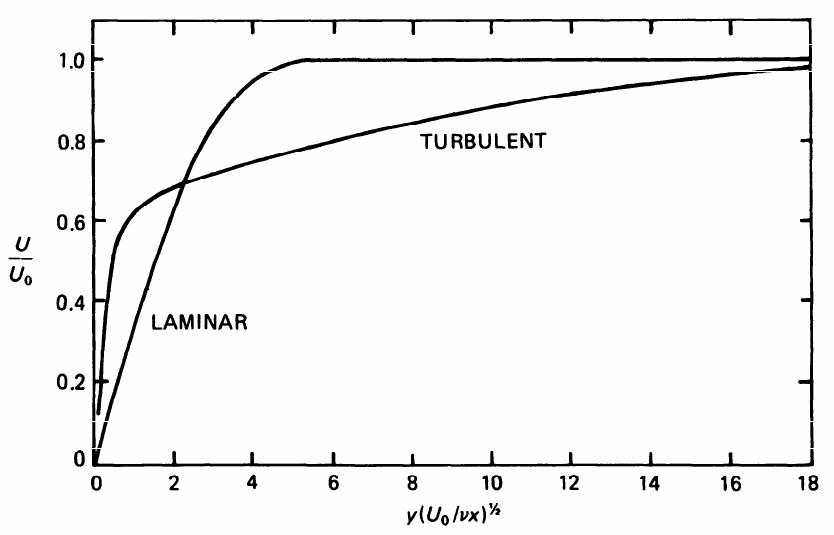
\includegraphics[scale=0.7]{captura.png}
    \caption{Comparación de una capa límite laminar y turbulenta. Fuente: \cite[Capítulo 21.5]{Tritton1988-ei}.}
    \label{fig:capturon}    
\end{figure}

Por otra parte, en la cámara de ensayo también debemos ser muy cuidadosos. La cuerda no debería ser superior a 
$\frac{1}{3}$ de la altura de la cámara \cite{Barlow1999-wm}. Aunque no se tienen medidas exactas, 
parece ser que la cuerda es menor a este valor. 
Por otra parte, para evitar el bloqueo de la corriente, el objeto de ensayo debe ser alrededor de un $5\%$ del área 
de la cámara de ensayo \cite{Barlow1999-wm}. Es posible que se supere este valor, lo que podría dar lugar a alguna interferencia.

De todas formas, sin llevar a cabo un ensayo más detallado tan solo se puede especular sobre el origen de estos errores.

\subsection{Posibles mejoras}

Una de las partes más débiles del trabajo es el cálculo de errores. Se trata de un temario en el que nunca hemos entrado 
en detalle. Se observa que los errores son enormes para todas 
las gráficas excepto las de $c_p$. Por una parte, esto parece tener sentido ya que se están propagando gran cantidad de errores,
pero estos errores aparentemente son demasiado grandes. Es posible que exista algún error teórico que está causando este problema.

Sí se repitiese el experimento, sería fundamental ser mucho más cuidadoso a la hora de ajustar 
los ángulos de ataque, que tienen una gran repercusión sobre la forma final de las curvas y sobre el error final. 

Otra mejora posible es la utilización de un lenguaje de programación más adaptado al mundo científico, como sería Python o R, o bien 
la colaboración con la multitud de desarrolladores que están trabajando en convertir Nim en un lenguaje apropiado para 
el cálculo científico. Por una parte, la librería \verb+ggplotnim+, utilizada para los gráficos, aún no ofrece todas las funcionalidades
que ofrece \verb+ggplot+ de R. Por otra parte, sería muy útil la utilización de una librería de propagación de errores para 
simplificar esta parte del trabajo, un buen ejemplo siendo \verb+uncertainties+, disponible para Python y portada a \verb-C++-, o una
librería equivalente. A día de hoy, no existe ninguna librería de propagación de errores para Nim, aunque se podría utilizar 
la de \verb-C++- a través de una capa de compatibilidad.

\section{Conclusiones}

El trabajo no solo ha servido como una primera experiencia con un túnel de viento, sino que ha sido una introducción al mundo
de la investigación aeroespacial. En un primer lugar, se ha permitido una gran libertad a la hora de realizar los cálculos. 
En parte, esta libertad ha creado una incertidumbre, que supongo estará también presente en la investigación real. Por otra parte,
ha permitido explorar las diferentes herramientas disponibles para este tipo de trabajos. 

También es importante añadir el choque que supone que los resultados experimentales coincidan muy mal con los resultados 
teóricos ofrecidos por X-Foil. Esta diferencia hace muy clara la necesidad de túneles de viento amplios, 
además de un protocolo riguroso y estricto a la hora de preparar los experimentos y tomar los datos.

Finalmente, la utilización de Nim ha demostrado algunas debilidades en cuanto a su utilización en el mundo científico,
aunque se compensa gracias a su simple y agradable sintaxis (similar a Python), junto a la poderosa librería estándar y su
alta velocidad al ser un lenguaje compilado, al contrario de Python o R.

\printbibliography

\end{document}